\documentclass[11pt,twoside,a4paper]{report}

% Intra-PDF Links and Bookmarks 
\usepackage[colorlinks=true,linkcolor=black,urlcolor=blue,bookmarksopen=true]{hyperref}
\usepackage[open,openlevel=1]{bookmark}

% A4, 1.91cm margins, header+footer
\usepackage[a4paper, margin=1.91cm, top=2.91cm, bottom=2.91cm]{geometry}
\usepackage{fancyhdr}
\pagestyle{fancy}
\fancyhf{}
\setlength{\headheight}{15.2pt}
\fancyfoot[LE,RO]{ \thepage }
\fancyfoot[RE,LO]{ \textit{Timothy Langer 2022} }

% Use UTF-8 so that we can have lots of nice characters!
\usepackage[utf8]{inputenc}
\usepackage[british]{babel}

% Maths symbols and packages
\usepackage{amsmath}
\usepackage{amssymb}
\usepackage{gensymb}

% easy way to include SI units in text
\usepackage{siunitx}

% Apply spacing in between paragraphs
\setlength{\parskip}{1em}
\setlength{\parindent}{0pt}

% Add diagrams and images support
\usepackage{graphicx}
\graphicspath{ {./images} }
\usepackage{caption}

% Mathematics typesetting support 
\usepackage{commath}

% Multiple columns
\usepackage{multicol}

% bibliography
\usepackage{csquotes}
\usepackage[
backend=biber,
style=numeric,
sorting=none,
urldate=long,
]{biblatex}

\addbibresource{./citations.bib}

%\usepackage[superscript,biblabel]{cite}

% better chapter titles
\usepackage[T1]{fontenc}
\usepackage{titlesec, blindtext}
\usepackage[usenames,dvipsnames]{xcolor}

% shorthands for custom chapter format
\colorlet{gray75}{gray!75}
% \definecolor{gray75}{gray}{0.75}
\newcommand{\hsp}{\hspace{20pt}}

% more compact chapter titles
\titleformat{\chapter}{\Huge\bfseries}{\thechapter\hsp\textcolor{gray75}{|}\hsp}{0pt}{\Huge\bfseries}
% less top/bottom padding around chapter titles
\titlespacing{\chapter}{0pt}{*0}{*1}

\usepackage{listings}

\lstset{
basicstyle=\scriptsize\ttfamily\color{black},
frame=single,
numbers=left,
numbersep=5pt,
numberstyle=\tiny\color{gray},
showspaces=false,
showstringspaces=false,
tabsize=1
}

\definecolor{dkgreen}{rgb}{0,0.6,0}
\definecolor{ltgray}{rgb}{0.5,0.5,0.5}

% https://github.com/cansik/kotlin-latex-listing
\lstdefinelanguage{Kotlin}{
  comment=[l]{//},
  commentstyle={\color{gray}\ttfamily},
  emph={filter, first, firstOrNull, forEach, lazy, map, mapNotNull, println},
  emphstyle={\color{OrangeRed}},
  identifierstyle=\color{black},
  keywords={!in, !is, abstract, actual, annotation, as, as?, break, by, catch, class, companion, const, constructor, continue, crossinline, data, delegate, do, dynamic, else, enum, expect, external, false, field, file, final, finally, for, fun, get, if, import, in, infix, init, inline, inner, interface, internal, is, lateinit, noinline, null, object, open, operator, out, override, package, param, private, property, protected, public, receiveris, reified, return, return@, sealed, set, setparam, super, suspend, tailrec, this, throw, true, try, typealias, typeof, val, var, vararg, when, where, while},
  keywordstyle={\color{NavyBlue}\bfseries},
  morecomment=[s]{/*}{*/},
  morestring=[b]",
  morestring=[s]{"""*}{*"""},
  ndkeywords={@Deprecated, @JvmField, @JvmName, @JvmOverloads, @JvmStatic, @JvmSynthetic, Array, Byte, Double, Float, Int, Integer, Iterable, Long, Runnable, Short, String, Any, Unit, Nothing},
  ndkeywordstyle={\color{BurntOrange}\bfseries},
  sensitive=true,
  stringstyle={\color{ForestGreen}\ttfamily},
}

\lstset{%
  	backgroundcolor=\color{white},
  	basicstyle={\footnotesize\ttfamily},
  	breakatwhitespace=false,
  	breaklines=true,
  	captionpos=b,
  	commentstyle=\color{dkgreen},
  	deletekeywords={...},
  	escapeinside={\%*}{*)},
  	extendedchars=true,
  	frame=single,
  	keepspaces=true,
  	keywordstyle=\color{blue},
  	language=SQL,
  	morekeywords={*,modify,MODIFY,...},
  	numbers=left,
  	numbersep=15pt,
  	numberstyle=\tiny,
  	rulecolor=\color{ltgray},
  	showspaces=false,
  	showstringspaces=false, 
  	showtabs=false,
  	stepnumber=1,
  	tabsize=4,
  	title=\lstname
}

\usepackage{pdfpages}

\newcommand\invisiblesection[1]{%
  \refstepcounter{section}%
  \addcontentsline{toc}{section}{\protect\numberline{\thesection}#1}%
  \sectionmark{#1}}

\pdfsuppresswarningpagegroup=1

\author{Timothy Langer}
\title{Smartphone-based tracking of rowing training}
\date{\today}

% this defines the \@title, \@author and \@date commands
\makeatletter

\fancyhead[LE,RO]{ \@title }

\begin{document}

\begin{titlepage}
  \centering
  \vspace*{1cm}
  {\bfseries \huge \@title \par}
  \vspace{2cm}
  {\large AQA Computer Science A-Level \par Non-Examined Assessment \par}
  \vspace{1.5cm}
  {\LARGE \@author \par}
  \vfill
  
\includegraphics[width=0.2\textwidth]{sps-logo} \par
  {\scshape\LARGE St Paul's School \par}
  Dr~C.~A.~Harrison \par
  \vspace{1cm}
  {\large \@date \par}
  \vspace*{1cm}
\end{titlepage}

% end the titling area
\makeatother

\tableofcontents

\chapter{Introduction}

Rowing in its modern form developed in England at the start of the 18th century, with the first recorded race held in $1715$. 
Nowadays, it is particularly popular in the UK and US. 
The Boat Race on television has over seven million viewers, with a further $250,000$ attending in person.\cite{the_boat_race} 

Two kinds of competitions exist: head races and regattas. 
A head race is one where competitors compete for the fastest time take to row a given distance. 
The outcome of the race is not clear until the race is over and times for every boat have been compiled.
A regatta involves side-by-side racing, across several lanes, usually over a course of $2000 \si{\meter}$.
Head races are typically of significantly longer distance (School's Head is roughly $7$km, for exmaple) and so pacing is particularly important.

\section{The rowing stroke}

\begin{figure}[ht]
    \centering
    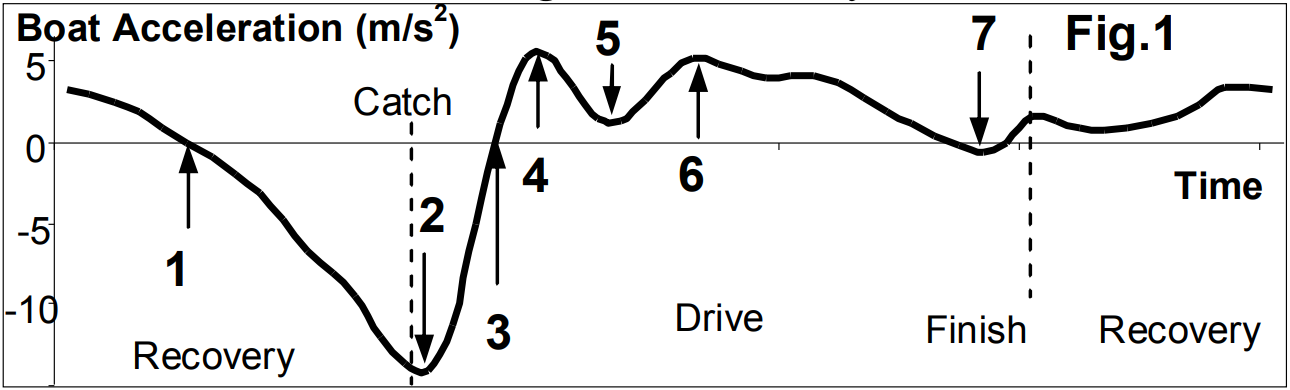
\includegraphics[width=0.7\textwidth]{rowing-stroke}
    \caption{Typical pattern of boat acceleration during the stroke cycle \cite{dr_valery_kleshnev_analysis_2012}}
    \label{fig:rowing-stroke}
\end{figure}

Rowing (and/or sculling) involves the propulsion of a racing shell\footnote{the long, light and narrow boat used for rowing} through the water, using either one or two oars. 
Rowing is cyclic and repetitive in its nature; every stroke is alike. 
The rowing stroke consists of two phases: the \textit{drive} and the \textit{recovery}. 
During the drive, the athelete pushes with their legs, moving towards the bow of the boat, with the oars in the water, thus accelerating the boat.
In the recovery, the athlete slides to the rear of the boat, while the boat slightly decelerates.
Figure \ref{fig:rowing-stroke} shows a typical acceleration pattern of a single stroke.

This acceleration pattern repeats with little fluctuation; thus one can determine the period with which it repeats and calculate the number of strokes being taken per minute. By combining this data with GPS readings, one can also calculate the distance the boat travels per stroke.

\chapter{Analysis}

\section{Identified issue}

A critical part of training is the \textbf{stroke rate}, which measures the number of strokes taken per minute of rowing. A higher stroke rate, with the same technique and power application, allows for more overall power to be applied per minute and thus move the boat faster. However, achieving a higher rate is difficult as the stroke length tends to shorten to compensate, especially as the rower fatigues. As such, many workout pieces are capped at a specified stroke rate, and it is necessary for the strokeman\footnote{the oarsman closest to the stern of the boat} and the cox\footnote{short for coxswain, the person steering the boat} to know the stroke rate of the boat and adapt the rowing stroke appropriately.

Another important part of training is the \textbf{split}, which measures the time taken, in minutes, to cover $500\si{\metre}$; in essence, it is the speed of the boat. Although the speed of the boat will vary with conditions such as wind and current, over the length of the course relative changes to the split during a rowing piece are good indicators of performance.

\section{Existing solutions}

\subsection{Simple solution}

Average stroke rate can be measured by counting the number of strokes taken in a minute. All that is necessary is  a stopwatch. This is a simple solution, but it is not very accurate. Additionally, the coxswain should be focusing on steering, not counting strokes!

The split of the boat can be calculated by manually measuring the time taken to cover a known distance of water. This solution makes it difficult to account for changes to the steering line, and does not allow for realtime feedback of the boat's speed.

\subsection{Rowing stopwatches}

\begin{figure}[ht]
  \centering
  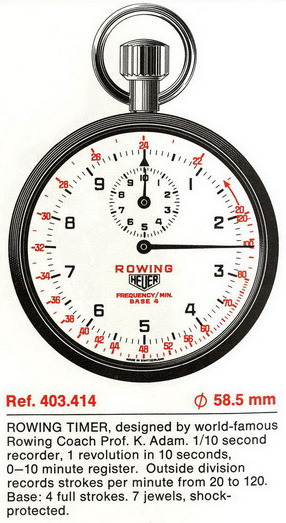
\includegraphics[width=0.3\textwidth]{rowing-stopwatch-heuer.jpg}
  \caption{A rowing stopwatch from the 1970-71 Heuer catalogue \cite{heuers_on_the_sea}}
  \label{fig:rowing-stopwatch-heuer}
\end{figure}

The 1960s saw the emergence of specialised rowing stopwatches. Figure \ref{fig:rowing-stopwatch-heuer} shows a rowing stopwatch manufactured by Heuer-Leonidas. These had a $1/10$th second resolution and were popular until the end of the 1980s. Repeated depressions of the crown at the same instant in each stroke provided a fully mechanical way of calculating the stroke rate.

\subsection{Nielsen-Kellerman StrokeCoach and SpeedCoach}

\begin{figure}[h!]
  \centering
  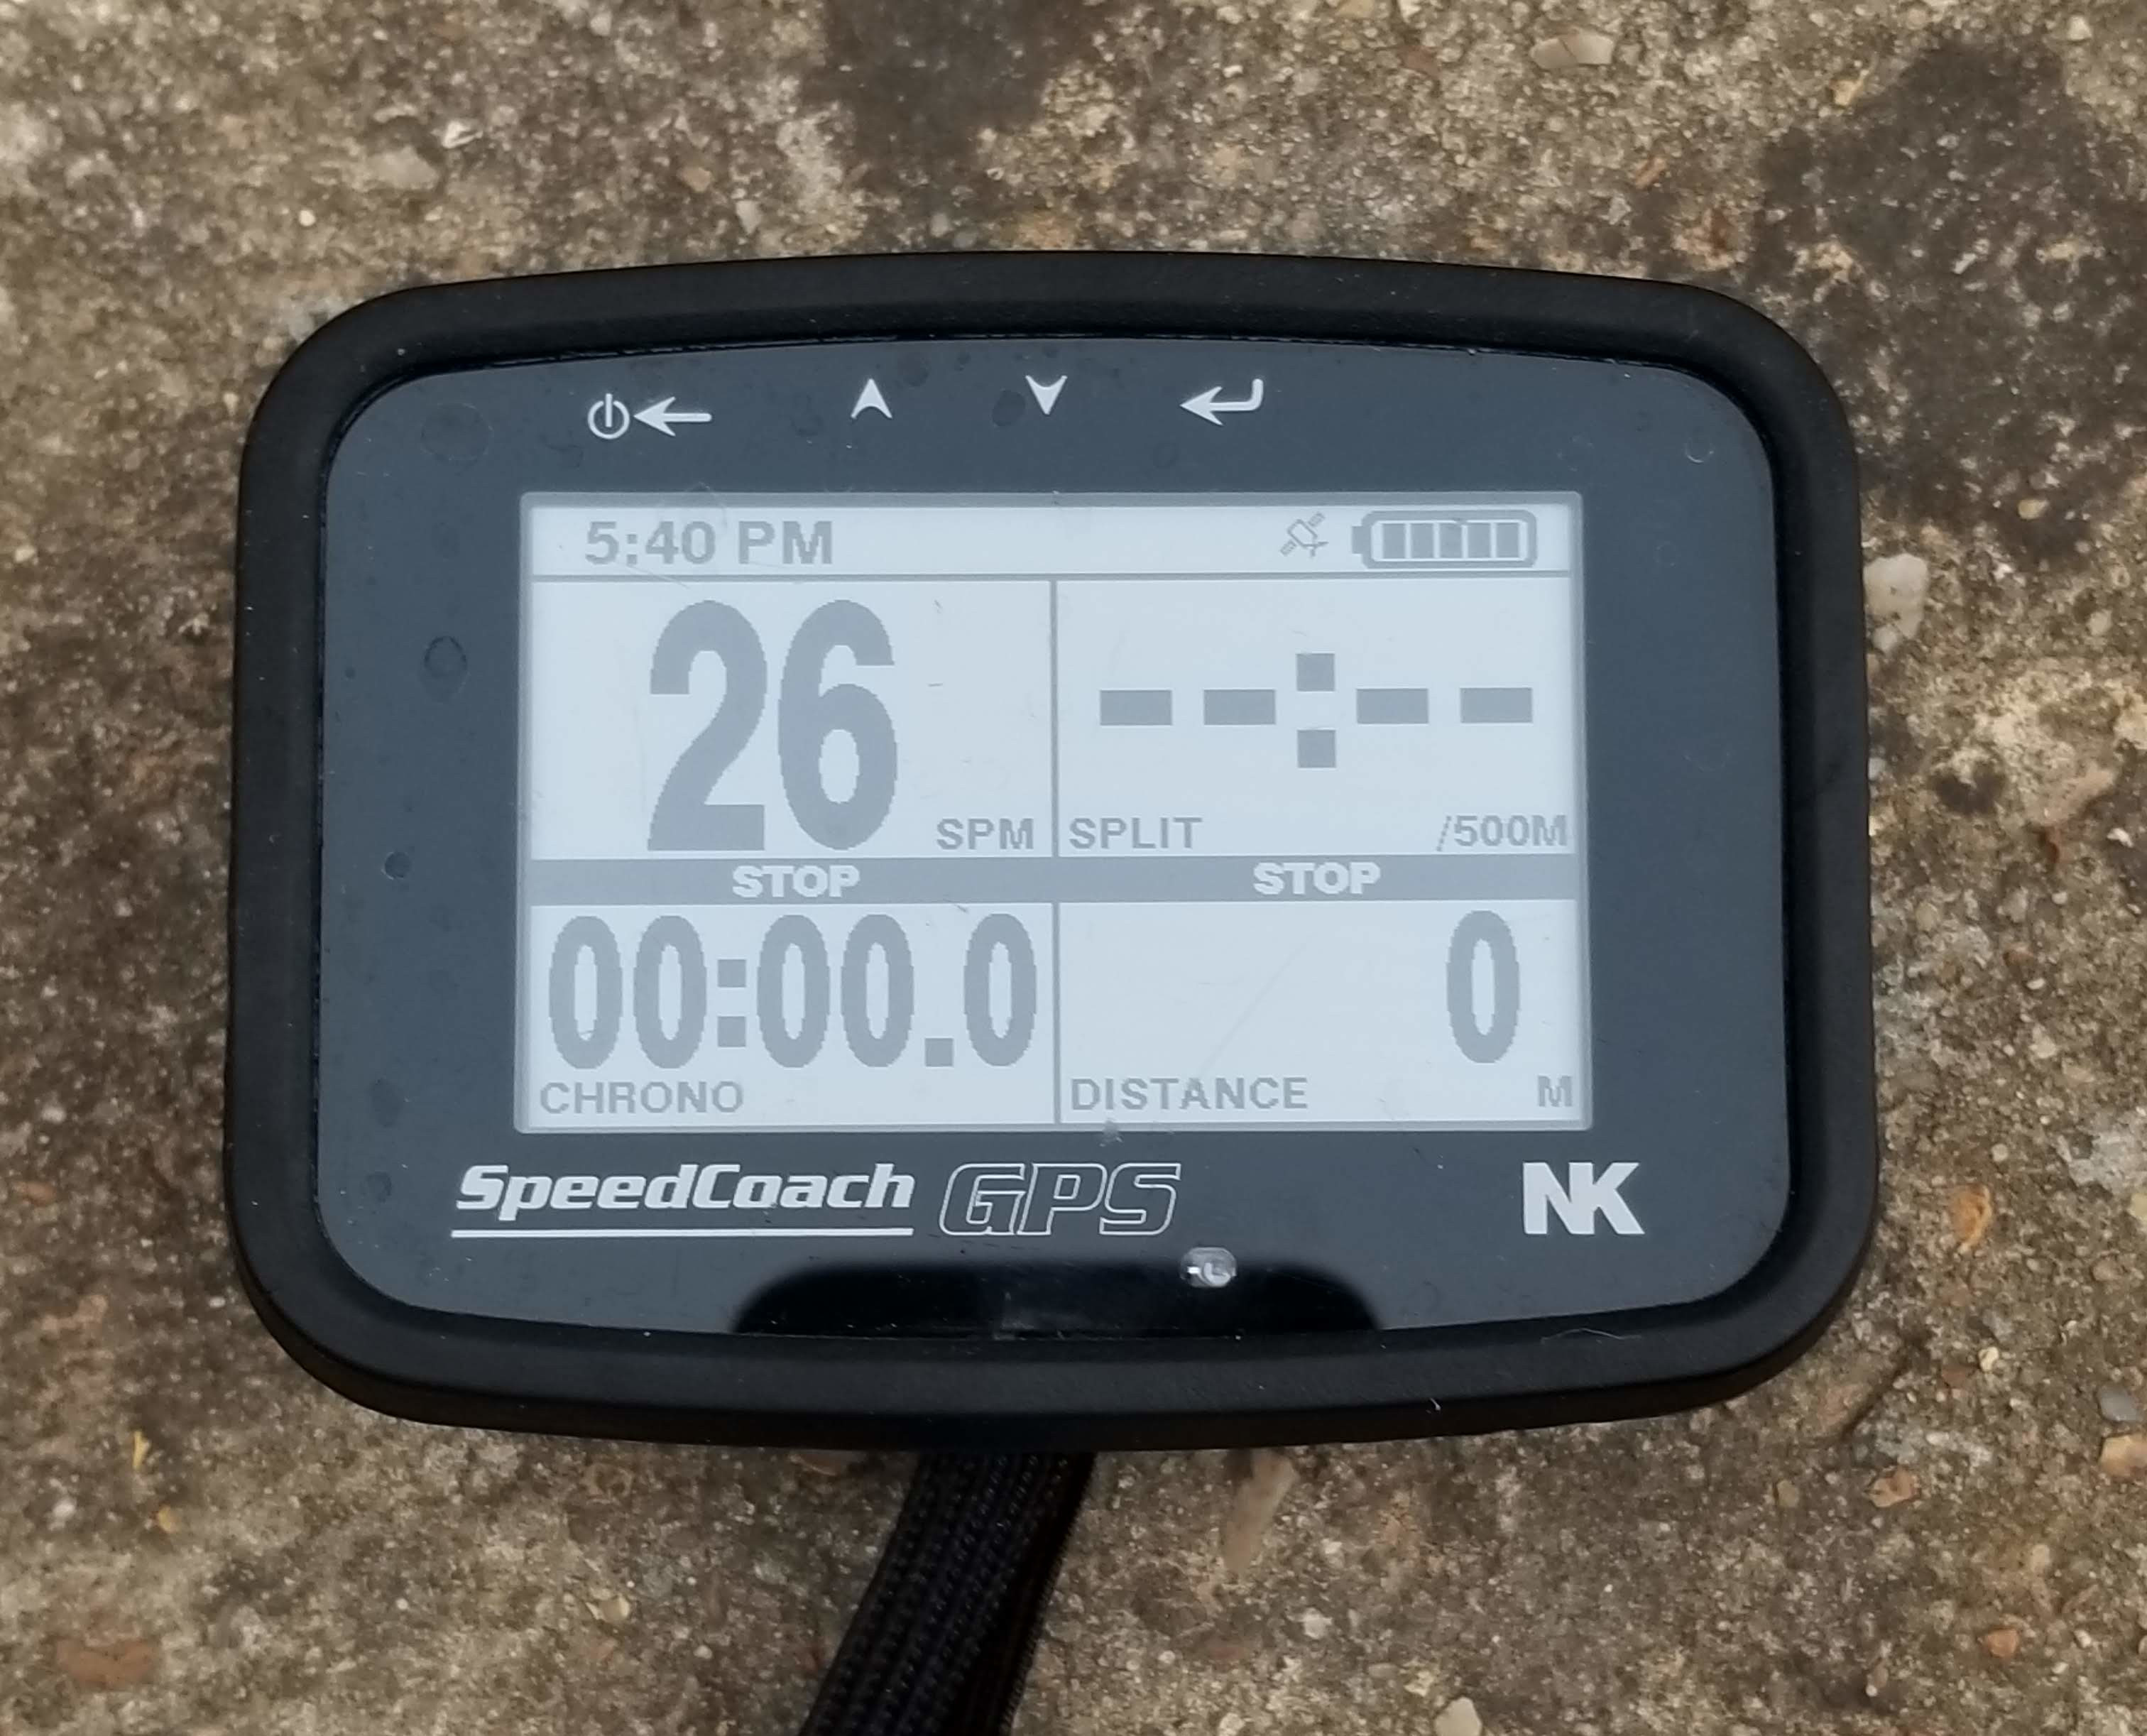
\includegraphics[height=0.4\textheight]{strokecoach.jpg}
  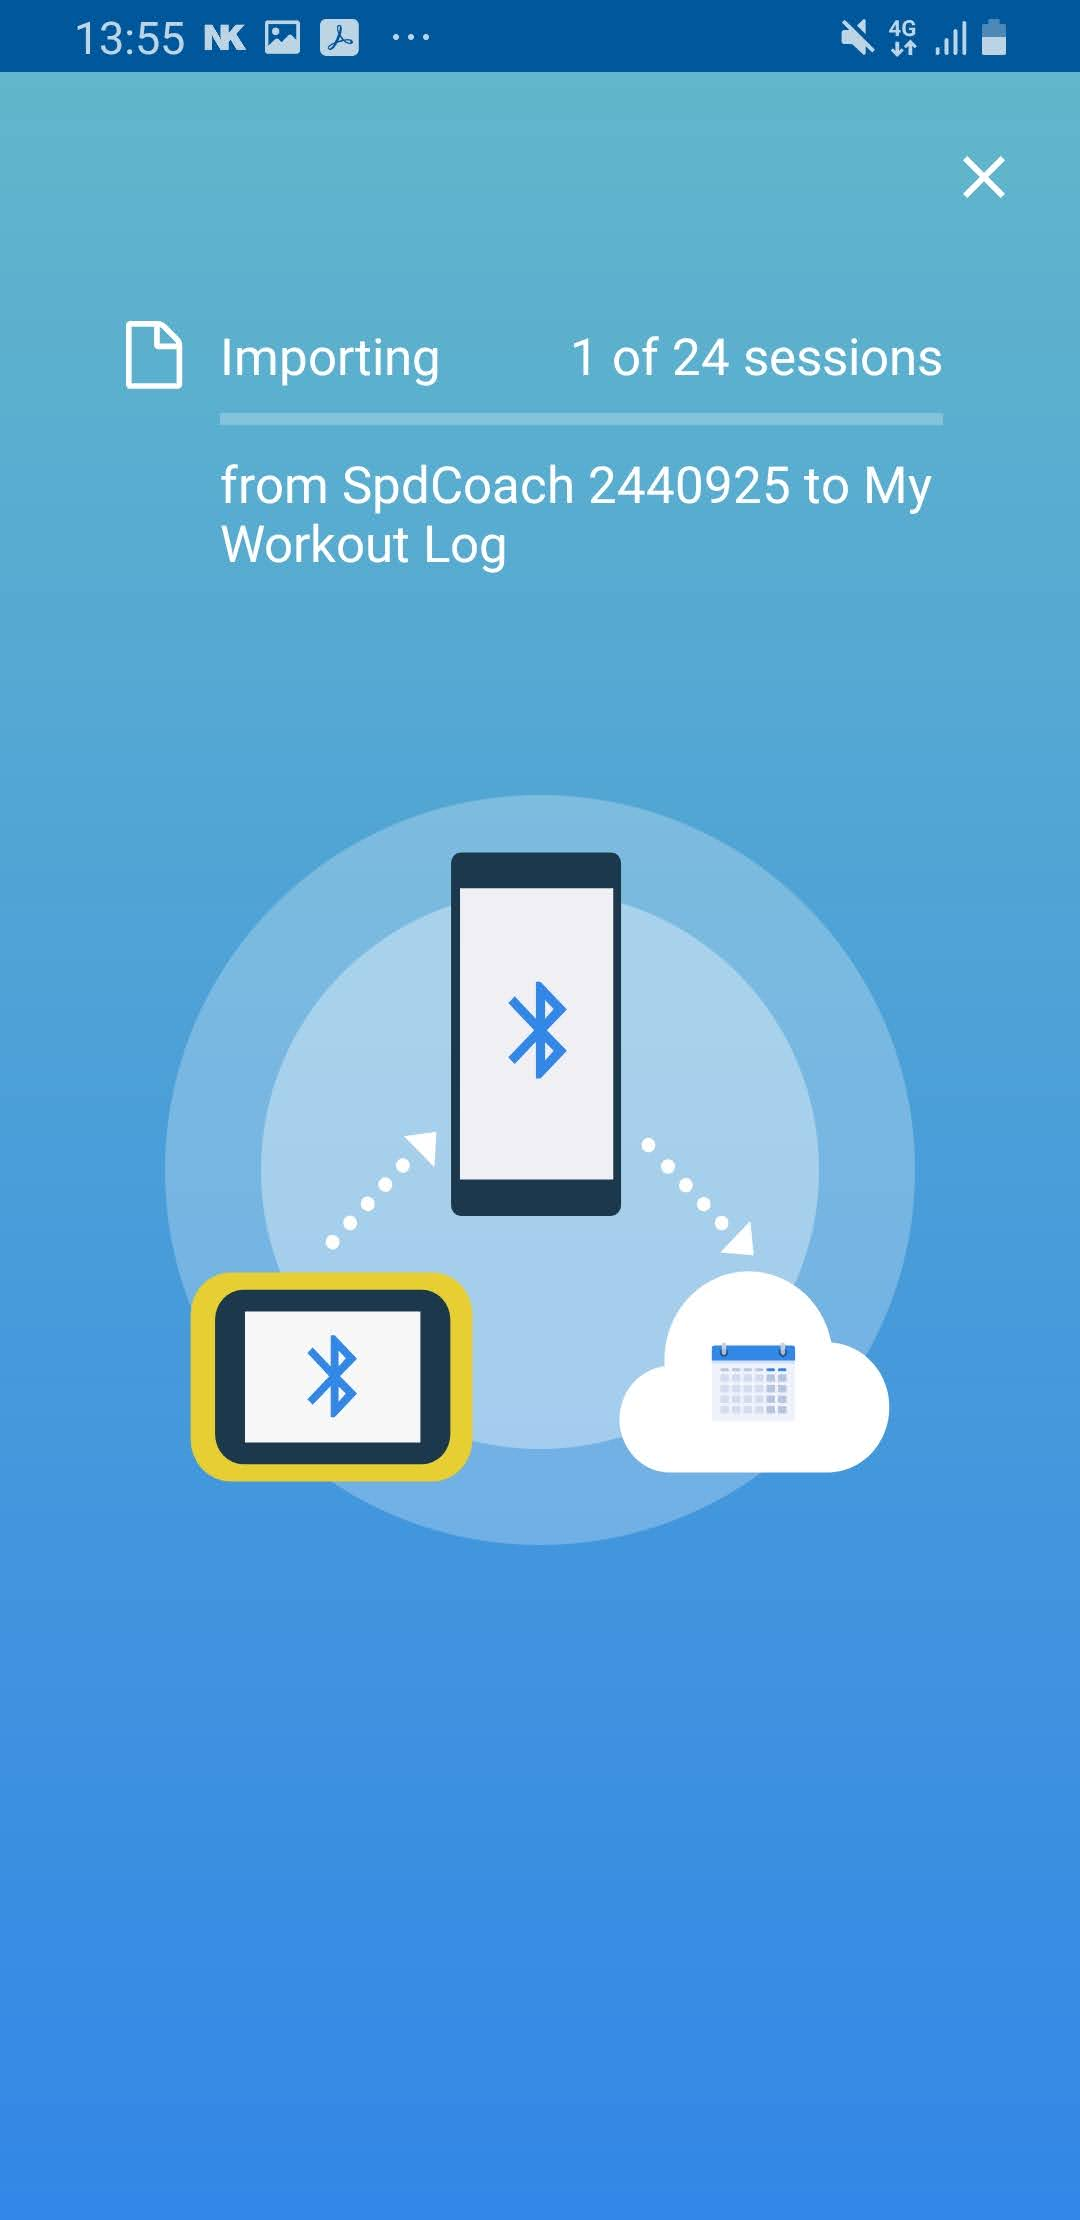
\includegraphics[height=0.4\textheight]{nklogbook.jpg}
  \caption{On the left is the NK SpeedCoach; on the right is a screenshot of the NK Logbook application synchronising 24 sessions off the SpeedCoach}
  \label{fig:nklogbook}
\end{figure}

The first NK stroke rate meter was released in 1984, known as the Chronostroke. This was an electronic device that doubled as a stopwatch and allowed the cox or the coxswain to calculate the stroke rate. The 1990s saw the first PaceCoach, which coupled with inboard and outboard sensors such as an impeller to calculate distance covered and real-time split.\cite{pacecoach}

The \href{https://nksports.com/speedcoach-gps-2}{NK SpeedCoach GPS (Model 2)} was released in 2012 and is a popular performance monitor for rowing on the water. 
It displays realtime information including split, stroke rate and the time and distance rowed. 
The first model used a physical magnet installed in the boat to record stroke rate, however, the second edition uses an inbuilt accelerometer for this and is completely wireless. 

An optional \textit{Training Pack} is available with Model 2 that adds software features such as Bluetooth support for heart rate monitor and synchronising training data to a smartphone.

The basic edition of the second model retails for \textsterling $399$; the \textit{Training Pack} is another \textsterling $99$.

Although the NK SpeedCoach is a popular rowing performance monitor, its price is certainly a barrier to entry. 

In addition, getting recorded data off the device is difficult, as Bluetooth connection is not reliable and requires synchronisation of \textit{all} the sessions on the stroke coach to obtain just the latest one.

\section{General solution statement}

The proposed solution, given the prevalence of smartphones in the modern world is a smartphone application that provides roughly equivalent core functionality to that of the commonplace NK SpeedCoach, including stroke rate, split and distance covered.

\section{Identified end user}

The end user is the coxswain or any of the rowers in the boat. In particular, the lower cost and availability of second-hand waterproof smartphones in comparison to the NK SpeedCoach would allow other rowers in the boat and not only the strokeman to be made aware of the rate. This solution would not be suitable for a coach in an adjacent boat, however, unlike a rowing stopwatch.

\section{Interviews}

\subsection{Interview with a rower}

An interview was conducted with the Captain of SPSBC, Sebastian Marsoner. \\ His answers have been paraphrased.
\begin{enumerate}
  \item What would you expect from a stroke coach application?
  
I would expect a stroke coach application to perform its most important task, determining the stroke rate, as accurately as possible. I have tried two different applications in an attempt to track my rowing, but neither of them could actually accurately tell me my stroke rate -- it seemed implausible, and as such I purchased a Nielsen-Kellerman SpeedCoach.

\item What features do you use on the SpeedCoach?

Usually I set it up to display my split, stroke rate, distance and heart rate. 

\item Do you feel the SpeedCoach solution is lacking in any areas?

Firstly, I would like to say that the SpeedCoach is great at what it does, although I am aware that it is rather expensive. Also, it has a rather limited memory and it is difficult to download the rowing sessions off the SpeedCoach. I would like to have a way to store all of my rowing sessions over time, so that I can compare a recent session with one from a previous year, for example, to better understand my progress.

\end{enumerate}

\subsection{Interview with a coxswain}

An interview was conducted with the SPSBC 1st VIII cox, James Trotman. \\ His answers have been paraphrased.
\begin{enumerate}
  \item What do you look for in a stroke coach?
  
  If I was to buy a stroke coach I would want it to
  \begin{itemize}
    \item be \textbf{accurate} so that the stroke rate and splits can be acted upon in realtime,
    \item be \textbf{cheaper} than currently available products such as the NK SpeedCoach,
    \item be \textbf{easy to use} so that as much time as possible is dedicated to training,
    \item integrate with other existing software to simplify the post-session review process.
  \end{itemize}

  \item You are familiar with the NK SpeedCoach and use it in your daily outings. \\ Which of its metrics do you use?
  
  The NK SpeedCoach has a four-panel display, so usually I set it up to display a stopwatch, the stroke rate, split and distance covered. In a race I usually swap the distance covered for distance per stroke but even then I rarely use it [the distance per stroke metric]. As a cox I do not need to see my heart rate and so do not use this feature.
  
  \item Is there any functionality that you feel the NK SpeedCoach is lacking?
  
  You can export rowing sessions off the SpeedCoaches, but it is not a simple task. Their app is buggy and the Bluetooth connection between my phone and the SpeedCoach is not always reliable. Also the synchronisation process requires one to download \textit{all} the sessions off the SpeedCoach even if you are only interested in the latest one.

  This might be harder to implement, but it would also be amazing to have power curve analysis like on the \href{https://www.rp3rowing.co.uk/}{RP3} on the water, and perhaps other metrics such as check\footnote{the sudden dip in boat velocity at the point when the oar enters the water} or ratio\footnote{refers to the relationship between the amount of time spent on the drive and the recovery}.

  \item You have also examined the data produced by the \href{http://biorow.com/}{BioRow} in-boat telemetry system. \\ Which of those additional metrics provided by BioRow you found useful?
  
  We found the graph of boat acceleration somewhat useful, as we were told that our boat acceleration at the catch is too shallow. However, it was not made clear what the optimal shape of the graph should look like. The \textit{verticle angle + boat roll} metric once again indicated to us that the boat was not level during our session, but we could easily tell that this was the case even before the telemetry system was installed.

\end{enumerate}

\section{Specific solution statement}

A smartphone application is to be designed; one that will inform the user of the stroke rate and split and split of the boat in real time. It will also show the elapsed time and the distance covered during a rowing session. Rowing sessions can be recorded for later viewing. 

Most people already have a smartphone with an accelerometer and a GPS sensor, which can be used to obtain data about the boat. In addition, since the tracking would be taking place on the phone itself, the need for synchronising sessions between a phone and a stroke coach would be eliminated.

\subsection{Practical considerations}

Although increasingly common, not all smartphones have a sufficient ingress protection rating to be comfortably taken into the boat. 
It is necessary to consider the requirement of a waterproof case, clamp or other holder that would allow the device to be affixed securely to the boat and prevent water damage in case of rain, waves or capsizing. 
One example would be a waterproof jogging armband: these are inexpensive, can be wrapped around a wing rigger \footnote{modern version of an \href{https://en.wikipedia.org/wiki/Outrigger}{outrigger} that spans across the middle from one saxboard to the other} and are a low barrier to entry.

\subsection{Device hardware}

Almost all handheld Android smartphones have an accelerometer, since this is necessary for the screen auto-rotation feature, and many also feature either a gyroscope or a magnetometer.\cite{android_motion_sensors} 
The key component for this project is the accelerometer, however, the gyroscope and magnetometer could be used to improve the accuracy of the data.

The top $1822$ most popular Android devices on Geekbench, a popular benchmarking tool, have an average performance of $1018$, scoring slightly higher than a desktop Intel\textsuperscript{\textregistered} Core\texttrademark i$3$-$8100$ CPU. \cite{android_benchmarks} However, we cannot rely on such performance. If this application is to appeal to rowing clubs as a viable alternative to the NK SpeedCoach, it cannot require an equally-priced smartphone to run! Therefore the core features of this app must be optimised to perform well on lower-end devices.
Efficient algorithms reduce strain on the CPU and thus make the process more battery-efficient.

\subsection{Programming languages and frameworks}

There are three primary supported programming languages for developing Android apps: C++, Java and Kotlin. Kotlin is a modern statically typed programming language used by over $60\%$ of professional Android developers. It is selected for this project due to the following advantages: 
\begin{itemize}
  \item Kotlin is cross-compatible with Java code, so although the language is relatively new, any libraries and frameworks developed for Java will work with Kotlin.
  \item Kotlin has many modern language features that draw inspiration from functional programming and allow for more concise code.
  \item Kotlin's coroutine functionality makes asynchronous programming simple and more efficient.
  \item Kotlin makes handling nullability of variables and objects far easier, to help avoid Java's dreaded \texttt{NullPointerException}. 
\end{itemize}

(From the \textit{Android Developers} website \cite{android_and_kotlin})

\subsection{Specification}\label{sec:spec}

A detailed specification is defined here that will be used to define the resulting application and the underlying technology.

The program \textbf{must}:
\begin{enumerate}
  \item be an application installable on any modern\footnote{released within the last five years} Android smartphone,
  \item require minimal configuration and interaction from the end user, and ideally none at all,
  \item be as easy to use and self-explanatory as possible for a new user,
  \item calculate the following metrics, as accurately as possible:
  \begin{itemize}
    \item the boat's stroke rate,
    \item the boat's split,
    \item the total distance rowed over the course of the session,
    \item the elapsed total session time,
  \end{itemize}
  \item display the above metrics in a realtime and an easy-to-read manner,
  \item collect data during a rowing session using nothing but the hardware on the smartphone,
  \item provide start/stop functionality to record the rowing session for later review,
  \item allow the user to export the recorded rowing session as a \href{https://developer.garmin.com/fit/file-types/activity/}{\texttt{FIT} activity file} that can be imported into 3rd-party software, such as \href{https://strava.com}{Strava}, containing
  \begin{itemize}
    \item the geolocation of the boat,
    \item the speed of the boat,
    \item the cadence, or stroke rate, of the rowers,
    \item the estimated power generated by the rowers
  \end{itemize}
  \item be as battery-efficient as possible
\end{enumerate}

\chapter{Design}

\begin{figure}[h!]
  \centering
  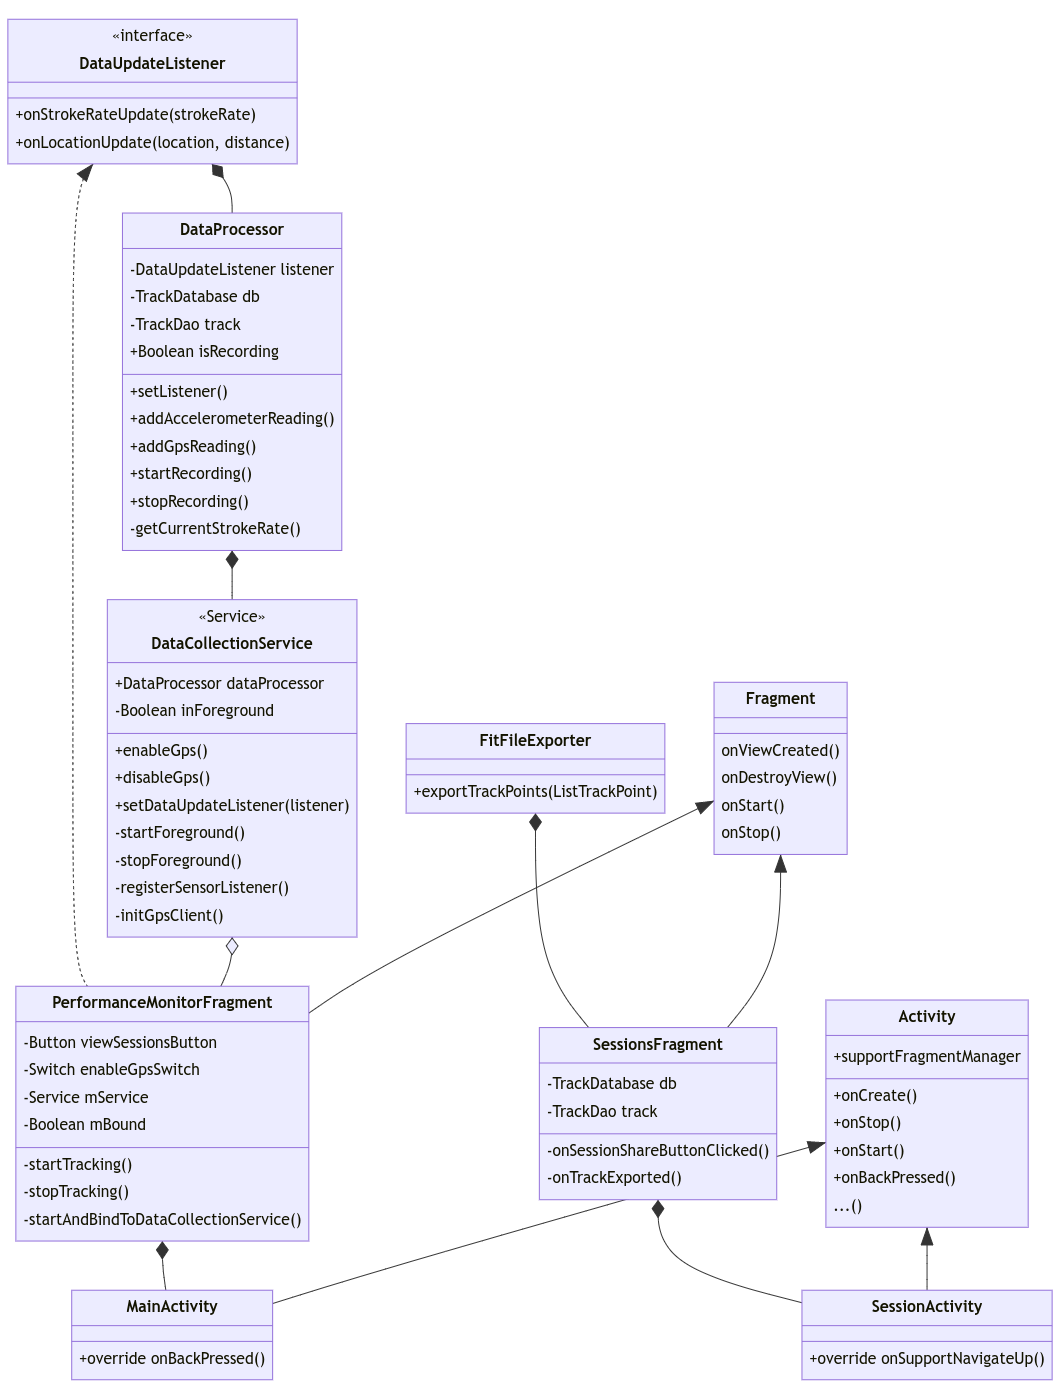
\includegraphics[width=0.8\textwidth]{umldiagram.png}
  \caption{UML diagram overview of the project}
  \label{fig:umldiagram}
\end{figure}


\section{Data collection}

\subsection{The data collection service}

Data collection and aggregation is to be performed in a service separate from the data processor and any UI classes. This is to ensure that the data collection service is always running, and that the data processor is always ready to process the data. It allows for the tracking to be decoupled from the user interface, so that even if the user interface goes out of view (e.g. the user exits to the home screen) during a rowing session, the recording process is not interrupted. 

The data collection process has the following primary objectives:
\begin{itemize}
  \item Manage its own lifecycle to prevent the tracking process from being killed by the OS
  \item Handle registration of sensor listeners, which are used to receive hardware sensor data.
  \item Appropriately handle the permission checks and requests required by the GPS client
  \item Pass on accelerometer and GPS measurements to a data processing class
\end{itemize}

\section{Processing incoming data}

\subsection{Stroke rate}

As part of the Android software stack, a virtual sensor is available that filters out acceleration due to gravity from the raw signal produced by the accelerometer.\cite{android_linear_accel} 

The acceleration and linear acceleration sensors output a vector with $x$, $y$ and $z$ axes, which are oriented relative to the device, with the $z$-axis coming out of the screen of the device. 
Since the boat is travelling linearly and we do not need an accurate numeric value for the accleration, it is enough to calculate the magnitude of the linear acceleration
\[
  \abs{\textbf{a}} = \sqrt{x^2 + y^2 + z^2} 
\] 
to obtain a repeating (with slight variation) pattern. Since we are taking the magnitude, the phone can be placed in any orientation and stroke rate detection can still be performed. Or, if the phone for example slips or changes position during the rowing session, stroke rate detection would not be interrupted. 

The shape of the acceleration readings produced by the above equation should are assumed to be similar in pattern to the absolute value of the acceleration pattern shown in in figure \ref{fig:rowing-stroke}.

\subsubsection{Filtering noise from the accelerometer}

\begin{figure}[h!]
  \centering
  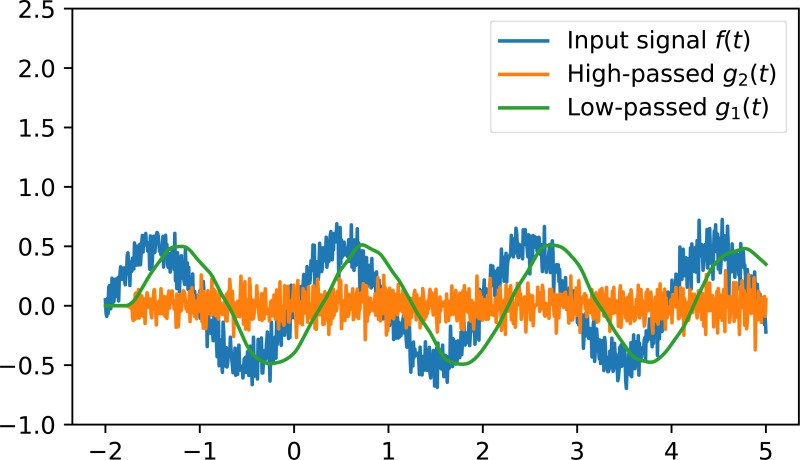
\includegraphics[width=0.6\textwidth]{lowpass-sine-ch2f15.jpg}
  \caption{Sine signal with additive noise after processing with a low-pass filter \cite{fischer_figure_2018}}
  \label{fig:lowpass}
\end{figure}

\begin{displayquote}
  A low-pass filter is a filter that passes signals with a frequency lower than a selected cutoff frequency and attenuates signals with frequencies higher than the cutoff frequency. (...) Low-pass filters provide a smoother form of a signal, removing the short-term fluctuations and leaving the longer-term trend. \cite{low-pass_2021}
\end{displayquote}

Many smartphone accelerometer sensors are not best-in-class so have significant noise. The application is to use a low-pass filter to remove the noise from the accelerometer readings through a procedure called ramping. This is a very efficient and simple way of smoothing the acceleration readings. However, the downside to this method is a slight phase shift in the signal, as visible in figure \ref{fig:lowpass}. At the standard accelerometer sampling rate of 50Hz this is not significant enough to cause substantial delay.

\label{filteringFactor}
The filter function $f$ is defined recursivley below, where $\textbf{a}_n$ is the last ($n$th) accelerometer reading as a three-dimensional vector and $k$ is the filtering factor, a constant determined empirically.
\begin{equation}\label{filterEqn}
  f \left( \textbf{a}_n \right) = k \textbf{a}_n + \left( 1 - k \right) f \left( \textbf{a}_{n-1} \right)
\end{equation}

\subsubsection{v1: Stroke rate by Fourier transform}

To calculate the stroke rate from the acceleration pattern, a Fourier transform is proposed. The Fourier transform is a discrete transform that can be used to calculate the frequency of a signal. It works by decomposing the sampled repeating pattern into a series of sinusoids. The frequency of the sinusoid with the greatest amplitude is selected as the true stroke rate. More specifically, a Sliding Discrete Fourier Transform (\textit{SDFT}) can be employed. The sliding DFT is a recursive algorithm to compute successive Fourier transforms of input data frames that are a single sample apart. It is an efficient $O(n)$ algorithm that can be used to calculate the frequency of a signal in real time.

\begin{displayquote}[from \textit{Sliding is Smoother than Jumping} \cite{sliding_smoother_than_jumping}]
  The idea behind the Sliding Discrete Fourier transform (SDFT) is to make use of the known values of $F_t(n)$, where $F_t(n)$ is the value in the $n$th bucket in the frequency domain, to calculate the value for the next window. In particular we assume that we are moving by one sample only.
  
  That means that in order to forget the oldest sample and accept a new sample, all that is needed is for the $n$th frequency amplitude is an addition, a subtraction and a complex rotation by $2\pi n / N$ radians. As we know that the samples are real this is a little simpler than it might appear.

  There remains the problem of starting, but if we assume that the signal was silent until the first sample, then the transform is also zero and so we can slide the samples in one at a time without creating an initial FFT [Fast Fourier Transform].


\end{displayquote}

The only necessary initialisation parameter for the SDFT is the window size $N$, which determines the number of frequency bins available. The maximal possible identifiable frequency is half the sample frequency according to Nyquist's theoreom, so this is used to determine the number of frequency bins available. A DC\footnote{DC for direct current, the frequency bin for the zero-frequency sinusoid} and Nyquist\footnote{the frequency bin for the maximal frequency} bin are also included, so the number of available frequency bins is $\frac{N}{2} + 2$.

\label{par:slideFreqBin}
Each frequency bin, in essence, is nothing more than a complex number. On each new sample these are altered appropriately. The sum of the real components of all the frequency bins is to be stored and recalculated on each addition of a new sample. This value is used to calculate the equivalent per-bin shift in value given the newly slid-in reading. The calculated shift in value is applied to each frequency bin in turn. [If there are $n$ frequency bins, this would require $n$ operations, which is what makes this algorithm $O(n)$.] 

A function is also to be provided to calculate the dominant frequency at the given moment in time which would return the wavelength of the frequency bin with the greatest magnitude when represented in polar form. This wavelength, in turn, can be used to calculate the stroke rate.

Although very efficient, unfortunately on implementation this Discrete Fourier Transform method was found to be lacking; the reasons for this are discussed on page \pageref{DFT_downsides}.

\subsubsection{v2: Stroke rate by autocorrelation}

Autocorrelation is a mathematical representation of the degree of similarity between a given time series and a lagged version of itself over successive time intervals. \cite{wiki_autocorrelation_2021}

The autocorrelation algorithm is to slide a copy of the second half of the data over itself, scoring each offset with the correlation of the slid data and the previous signal.

\label{par:autoCorAlgo}
The discrete autocorrelation $R$ at lag $\tau$ for a discrete time signal $X$ is given by
\begin{equation*}
  R(\tau) = \text{Corr}\left(X_n,\,X_{n-\tau}\right)
\end{equation*}
Correlation of two data sets $X$ and $Y$ is given by the below formula (from the Further Maths syllabus!)
\begin{equation*}
  \text{Corr}\left(X, Y\right) = \frac{\text{Cov}\left[X, Y\right]}{\sqrt{\text{Var}\left(X\right)\text{Var}\left(Y\right)}}
\end{equation*}
Since in this case $X$ and $Y$ are the same underlying data, except with different lag, their variances must be the same. The denominator can be simplified to $\text{Var}\left(X\right)$.

Expressing the covariance and variance as a summation, the below formula is obtained, where $\mu$ is the mean of the data.
\begin{equation}
  R\left(\tau\right) = \frac{\sum \left(X_i - \mu\right)\left(X_{i-\tau} - \mu\right)}{\sum \left(X_i - \mu\right)^2}
\end{equation}

$R$ is to be calculated for every possible value of $\tau$ up to half the window size. The value of $\tau$ that produces the maximal output for $R$ is selected as the most probable time period of the stroke rate, measured in a number of samples. By tracking the average accelerometer sampling rate as samples come in, the number of samples $\tau$ can be converted into a stroke rate.

\section{Data storage}

A SQL database is chosen to store the data. The database is to be used to store the the stroke rate, the location of the boat and the time of the readings. Each row in the database stores the mentioned quantities, as well speed of the boat at that instant, measured in metres per second. A separate column for speed allows for more accurate speed recordings than a simple $\frac{\text{distance}}{\text{time}}$ calculation. Each entry stores a unique point ID, as well as the ID of the session that it belongs to. The table called \texttt{records} is defined with the following schema:

\begin{lstlisting}[language=sql]
CREATE TABLE IF NOT EXISTS records (
  pointId INTEGER PRIMARY KEY AUTOINCREMENT NOT NULL,
  trackId INTEGER NOT NULL, 
  timestamp INTEGER NOT NULL, 
  stroke_rate REAL NOT NULL, 
  latitude REAL, 
  longitude REAL, 
  speed REAL
)
\end{lstlisting}

The query below retrieves the a list of session IDs present in the database and their corresponding starting timestamps. This query will be performed when a list of previously recorded sessions is shown to the user.
\begin{lstlisting}[language=sql]
  SELECT trackId, MIN(timestamp) 
  FROM records 
  GROUP BY trackId 
  ORDER BY timestamp DESC
\end{lstlisting}

The query below retrieves all of the track points for a given session ID, in this example $123$.
\begin{lstlisting}[language=sql]
  SELECT * 
  FROM records 
  WHERE trackId == 123 
  ORDER BY pointId ASC
\end{lstlisting}

\subsection{SQL Libraries on Android}

The Android Room library is part of the Android Jetpack collection of first-party libraries by Google. It is selected as the database library for this application due to the following convincing arguments:

\begin{displayquote}[extract from the official Android Developers Guide \cite{android_room_overview}]
  The Room persistence library provides an abstraction layer over SQLite to allow fluent database access while harnessing the full power of SQLite. In particular, Room provides the following benefits:

  \begin{itemize}
    \item Compile-time verification of SQL queries.
    \item Convenience annotations that minimize repetitive and error-prone boilerplate code.
    \item Streamlined database migration paths.
    \item Because of these considerations, we highly recommend that you use Room instead of using the SQLite APIs directly.
  \end{itemize}

\end{displayquote}

\begin{figure}[h!]
  \centering
  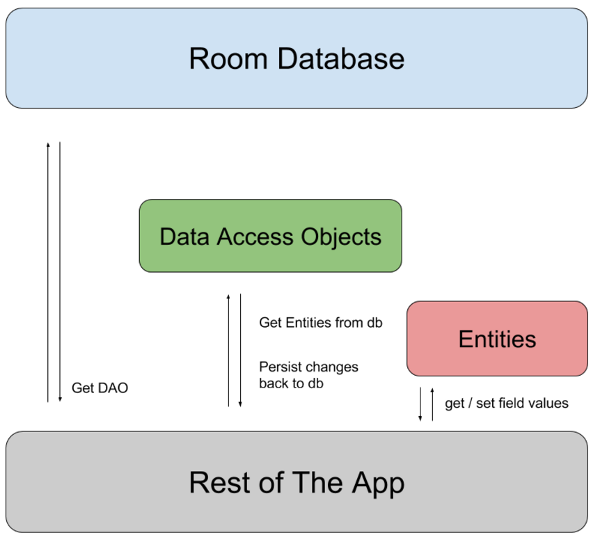
\includegraphics[width=0.6\textwidth]{roomarchitecture.png}
  \caption{Diagram of Room library architecture \cite{android_room_overview}}
  \label{fig:roomarchitecture}
\end{figure}

As per the Room architecture (as shown in figure \ref{fig:roomarchitecture}), creating a Room database requires three parts:
\begin{itemize}
  \item the database itself
  \item the data access objects which provide queries for interacting with the database
  \item entities which define the tables and columns in the database
\end{itemize}

These are defined in separate classes, so three classes \texttt{TrackDatabase}, \texttt{TrackDao} and \texttt{TrackPoint} are to be created. The \texttt{TrackDao} class will use the SQL queries described earlier in this section. The \texttt{TrackPoint} class will be used to store the data in the database.

\section{File export}

\begin{displayquote}[from the Garmin FIT SDK Overview \cite{garmin_fit_overview}]
The Flexible and Interoperable Data Transfer (FIT) protocol is designed specifically for the storing and sharing of data that originates from sport, fitness and health devices. The FIT protocol defines a set of data storage templates (FIT messages) that can be used to store information such as user profiles, activity data, courses, and workouts. It is specifically designed to be compact, interoperable and extensible.

The FIT file protocol was designed to provide:
\begin{itemize}
  \item Interoperability of device data across various platforms
  \item Scalability from small embedded devices to cloud platforms
  \item Forward compatibility, allowing the protocol to grow and retain existing functionality
  \item Automated compatibility across platforms of different native endianness
\end{itemize}

After the initial sensor data is collected, the FIT protocol provides a consistent format allowing all devices in the subsequent chain to share and use the data.



\end{displayquote}

When requested by the user, a given recorded rowing session should be exported as a FIT activity file. Garmin provides a FIT SDK in Java, which is cross-compatible with Kotlin. The FIT file type is chosen for its widespread support by sports software such as Strava. It is preferred to recording to, for example, a GPX file, since a FIT file has built-in support for additional metrics besides GPS, such as cadence and heart rate. Of course, a GPX file exporter could also be implemented but there is no such necessity if FIT export is available. There exists software such as FitCSVTool to convert a FIT activity file to a CSV file for analysis in spreadsheet software like Microsoft Excel.

\section{User interface}

\subsection{Main performance screen}\label{sec:pmfrag}

On fragment creation, the fragment is to perform a few initial user interface setup tasks (aside from actually inflating the layout of the UI components) including:
\begin{itemize}
  \item requesting the screen to not turn off even after the usual dimming time
  \item requesting the device to stay oriented in portrait mode, so that boat roll does not cause unnecessary screen rotation that could distract the rower
  \item configuring callback functions for the "view sessions" button, the GPS status switch and start/stop recording button
\end{itemize}

In addition, this fragment is to be responsible for starting up, where necessary, the data collection service and binding to it while the user interface is active. Once bound, the fragment, which implements the listener interface, can set itself as a callback listener in order to receive updates when a new stroke rate or split becomes available.

\subsection{Session history}

A separate view, accessible via a \textit{view sessions} button on the application home screen, takes the user to a screen where they can select a previously recorded session and export/share the session with another application on the device. The list of sessions is retrieved from the database and displayed in a list, with each row labelled with the session start time.

\chapter{Technical solution}

\section{Data collection}

The gathering and aggregation of collected data is handled by the \texttt{DataCollectionService}. This service is started when the application is started. It is run as service, and as such inherits from the Android \texttt{Service} class.

\subsection{GPS}

The \texttt{initGpsClient} function is called within the service's \texttt{onCreate} method. This function initializes the GPS client, which is used to obtain the current location of the boat. The GPS client is configured to obtain a fix once a second, and to obtain the best possible accuracy. A \texttt{LocationCallback} is provided for the GPS client to call to notify the service when a new location is obtained. The callback passes the newly obtained location fix to the \texttt{DataProcessor}.

The \texttt{DataCollectionService} provides two functions to control whether GPS updates are to be requested. These functions, \texttt{enableGps} and \texttt{disableGps} are public and as such can be called by any class that binds to the running service. GPS collection is enabled by default, so the \texttt{enableGps} function is called in the service's \texttt{onCreate} method. The \texttt{disableGps} function is called in the service's \texttt{onDestroy} method so that the device ceases to request GPS location updates if/when the service is destroyed.

\subsection{Accelerometer}

The \texttt{DataCollectionService} implements the \texttt{SensorEventListener} interface, which allows it to receive sensor data from the Android hardware. The \texttt{onSensorChanged(event: SensorEvent)} method is called when a new sensor data is available. The \texttt{SensorEvent} object contains the sensor data, and in the case of the accleerometer, the \texttt{SensorEvent.values} array contains the acceleration readings as a three-dimensional vector. This array is passed to the \texttt{DataProcessor} for processing.

\subsection{Service Management}

Android has strict policies for long-running services with battery optimisation in mind. It is mandatory for the service to display a notification if the application interface is not visible to the user. This is why a significant portion of the \texttt{DataCollectionService} is dedicated to binding and unbinding from user interface classes and showing the service notification where appropriate. A private inner \texttt{NotificationUtils} class is responsible for actually creating the notifications that will be shown to the user to prevent cluttering the \texttt{DataCollectionService} class. Notifications are pushed by a coroutine task since this can take a non-neglible few milliseconds that can add up to a noticeable delay.

The code for the \texttt{DataCollectionService.kt} is displayed overleaf.

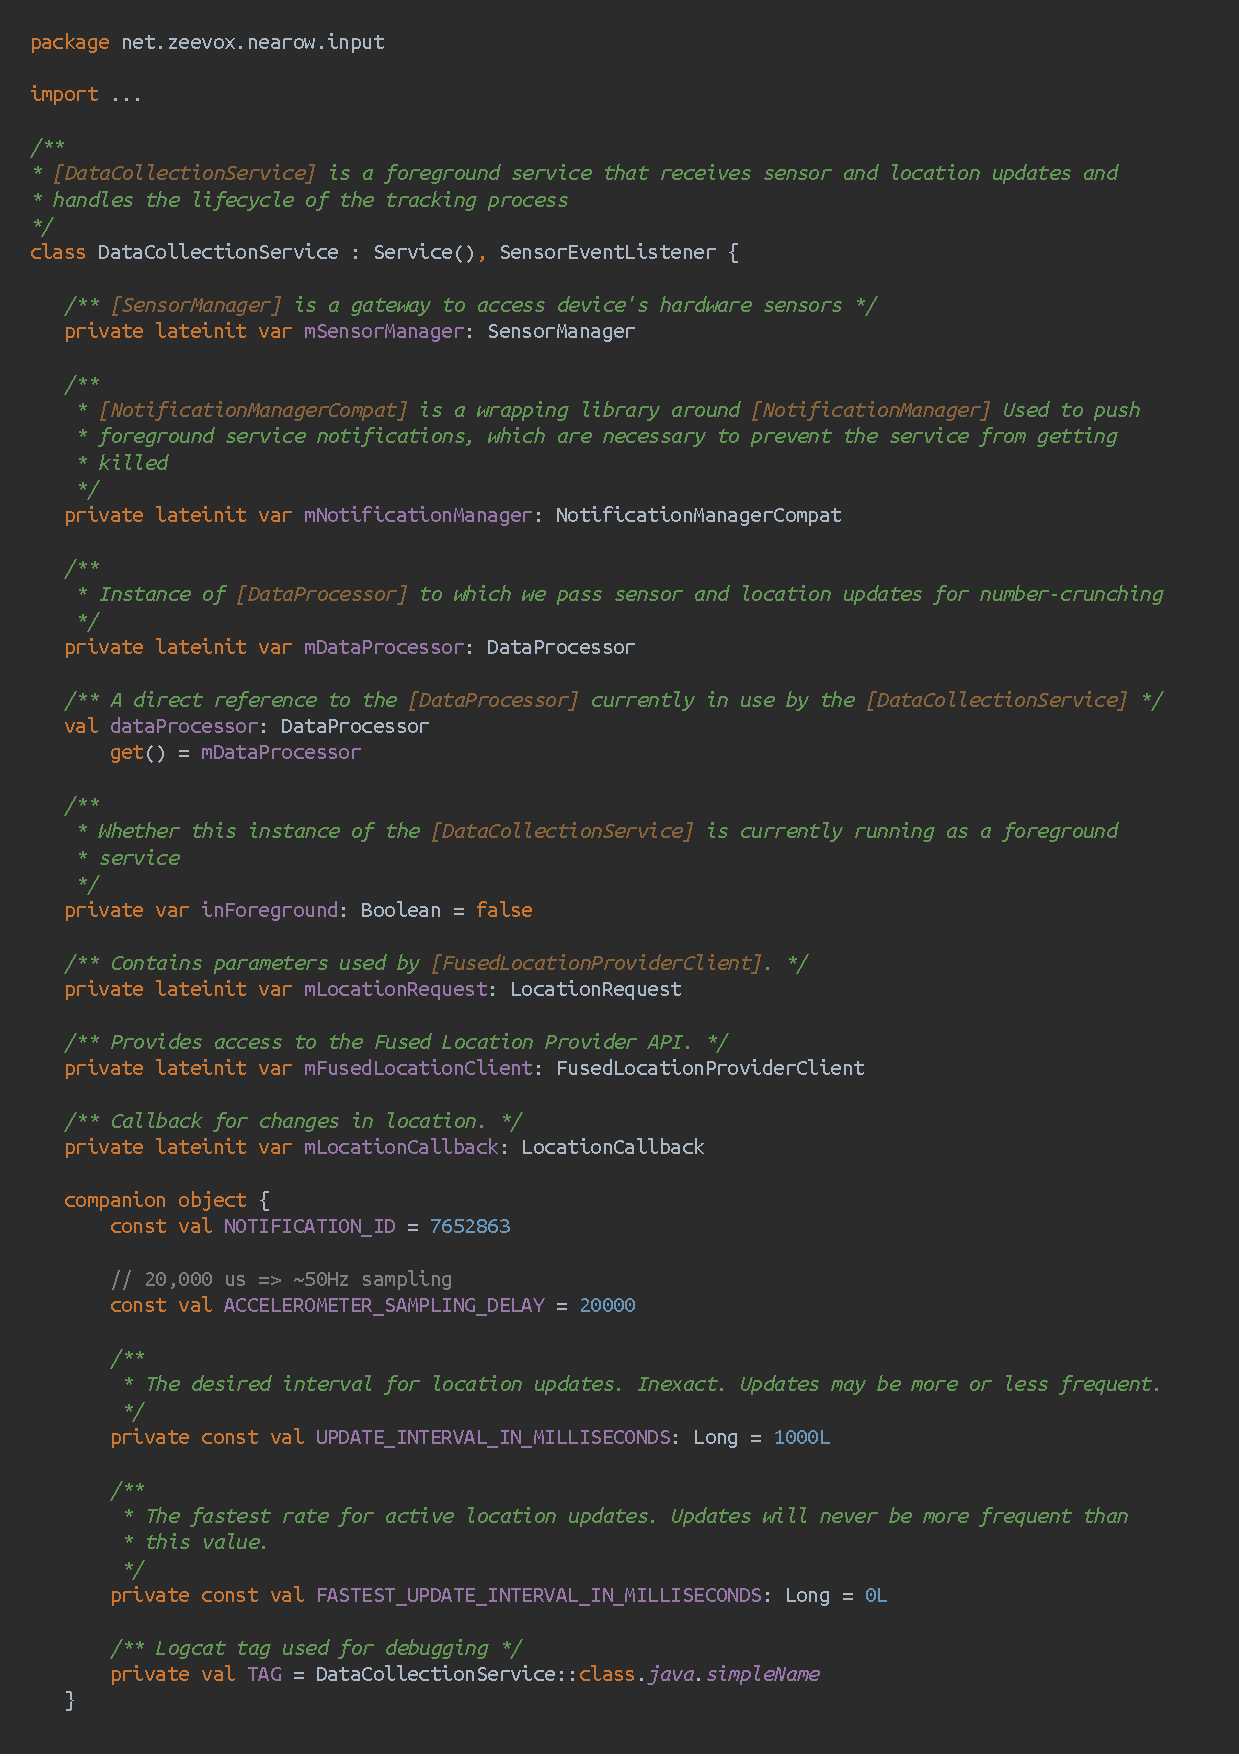
\includepdf[pages=-,pagecommand={},width=1.0\textwidth]{code/DataCollectionService.pdf}

\section{Data processing}

\subsection{\texttt{SlidingDFT.kt}}

As specified in the design stage, the incoming acceleration readings are to undergo a Sliding Discrete Fourier Transform (SDFT) to find the dominant frequency.

\begin{figure}[h!]
  \centering
  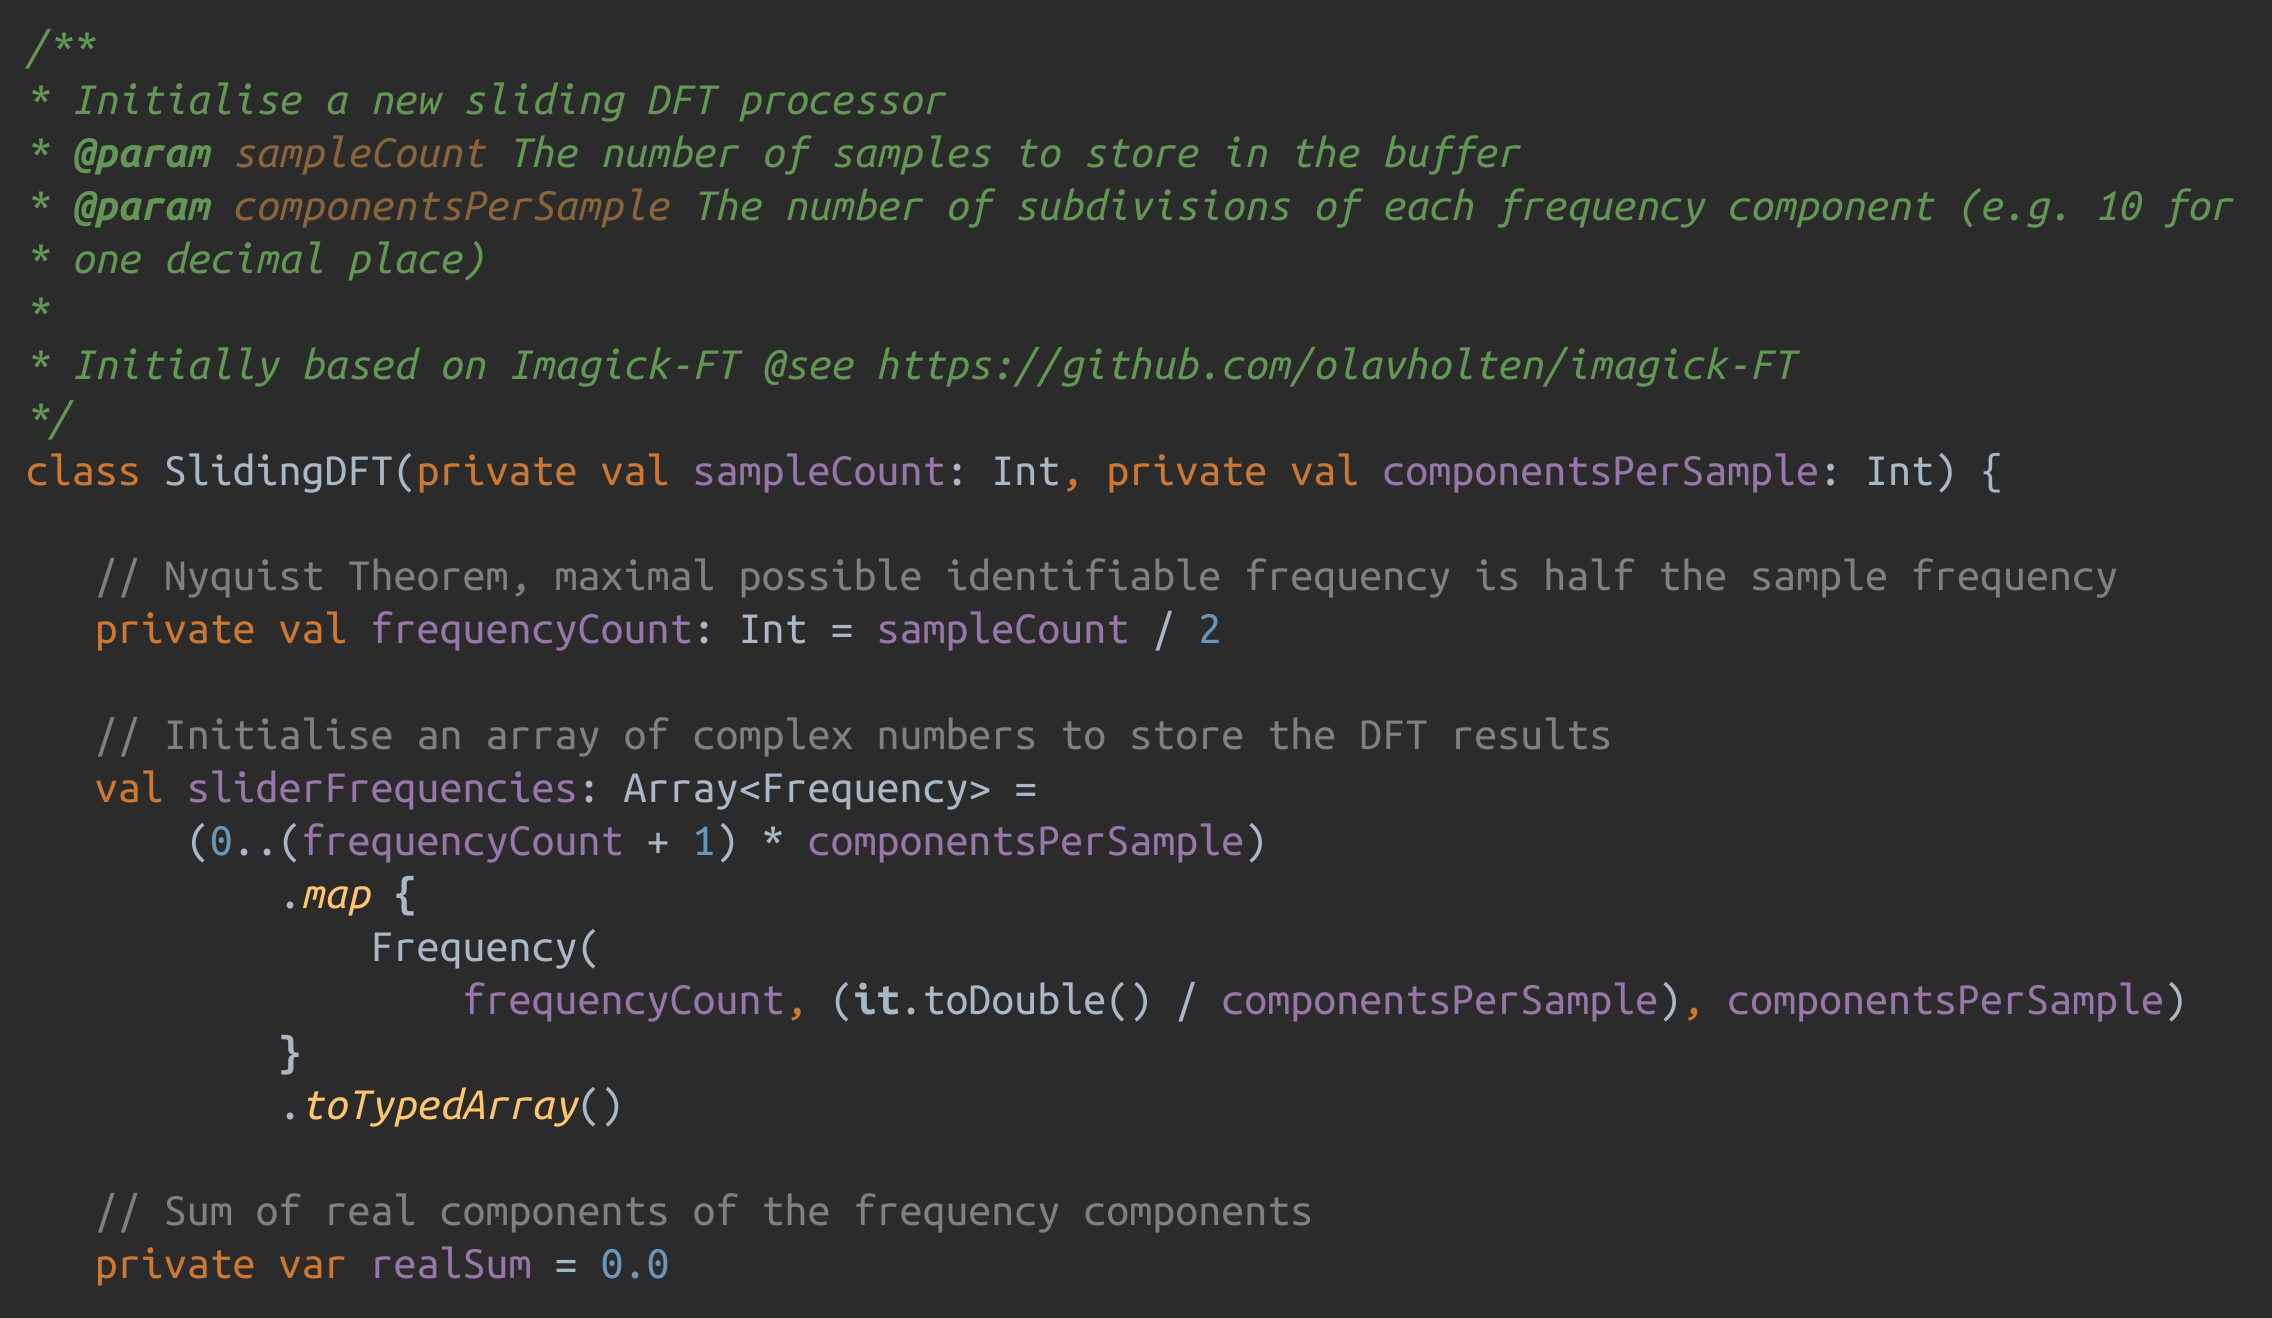
\includegraphics[width=0.9\textwidth]{code-slidingDFT.png}
  \caption{}
  \label{fig:slidingDFT}
\end{figure}

The \texttt{SlidingDFT} class is initialised with the number of successive samples to be used. The constructor and initialisation code is shown in figure \ref{fig:slidingDFT}. A later addition also includes a \texttt{componentsPerSample} parameter that allows for one to subdivide the frequency bins into a number of sub-bins to allow for greater frequency resolution at the expense of higher latency.

\begin{figure}[h!]
  \centering
  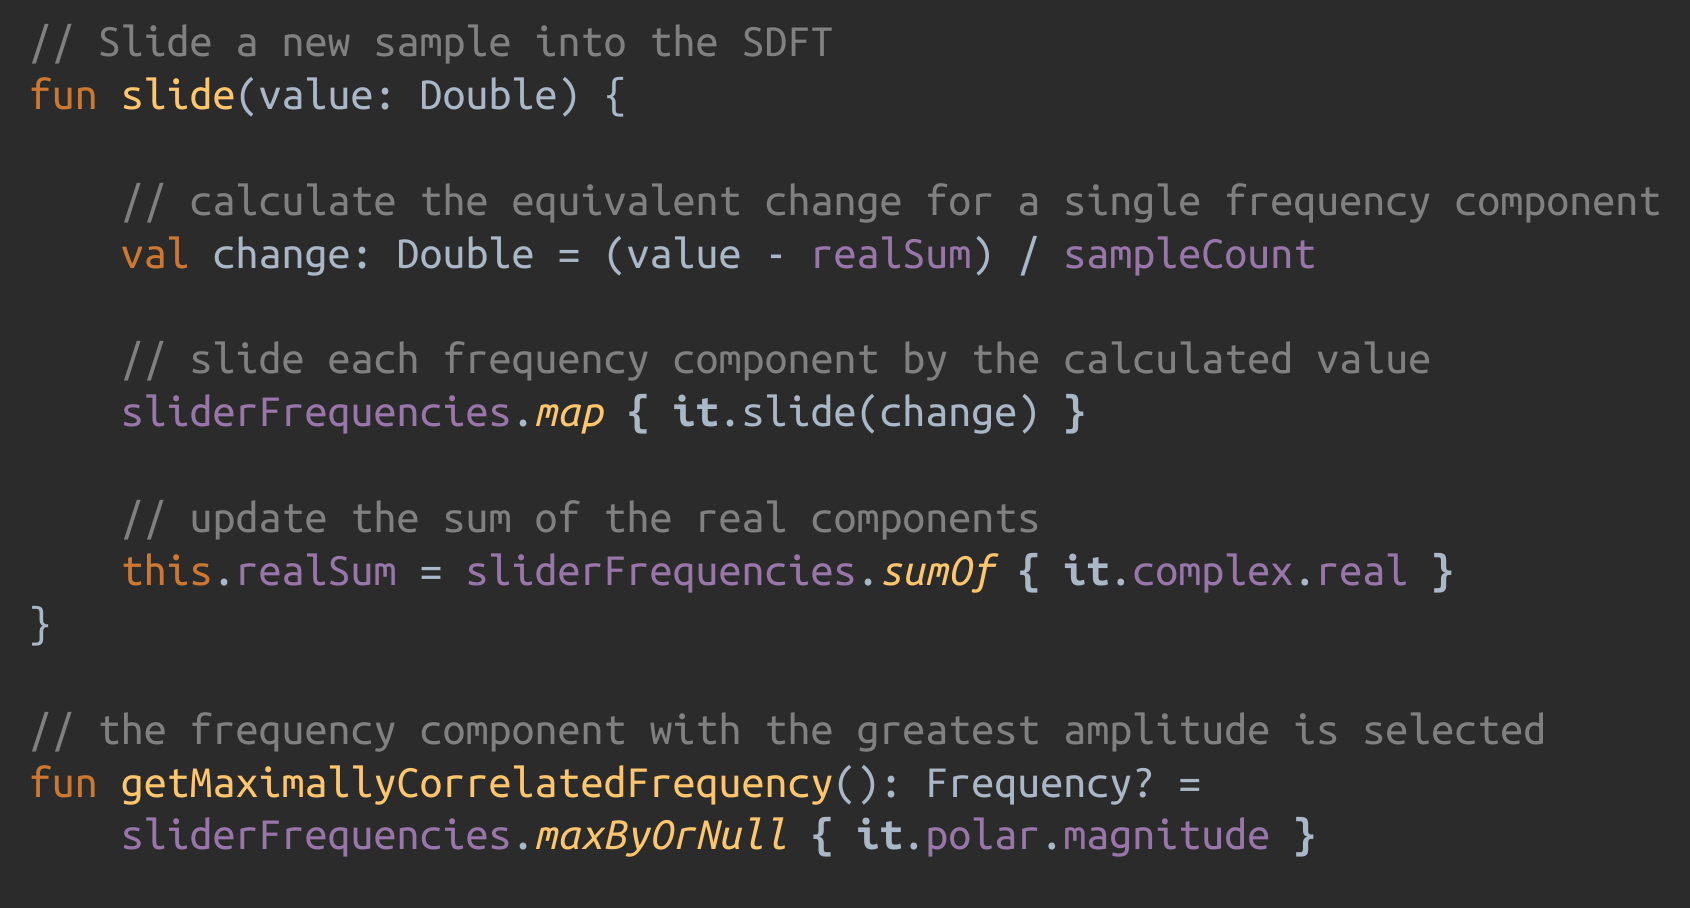
\includegraphics[width=0.8\textwidth]{code-SDFT-slide.png}
  \caption{\texttt{SlidingDFT} initialisation code}
  \label{fig:slideBest}
\end{figure}

Figure \ref{fig:slideBest} shows the code for the methods described on page \pageref{par:slideFreqBin}. The \texttt{slide} method is called when a new sample is available. The \texttt{getMaximallyCorrelatedFrequency} method is called when the stroke rate is to be updated.

Within the \texttt{SlidingDFT} class an inner class called \texttt{Frequency} is defined, the code for which is displayed in figure \ref{fig:innerClassFrequency}. This class represents a single frequency component of the SDFT. As stated in the paper, each frequency component experiences a rotation of $2\pi n / N$ radians, where $n$ is the wavelength and $N$ is the window size. Since we halved the window size to obtain the total number of frequency bins, the factor of $2$ cancels out. A correction is applied for DC and Nyquist frequency bins.

\begin{figure}[h!]
  \centering
  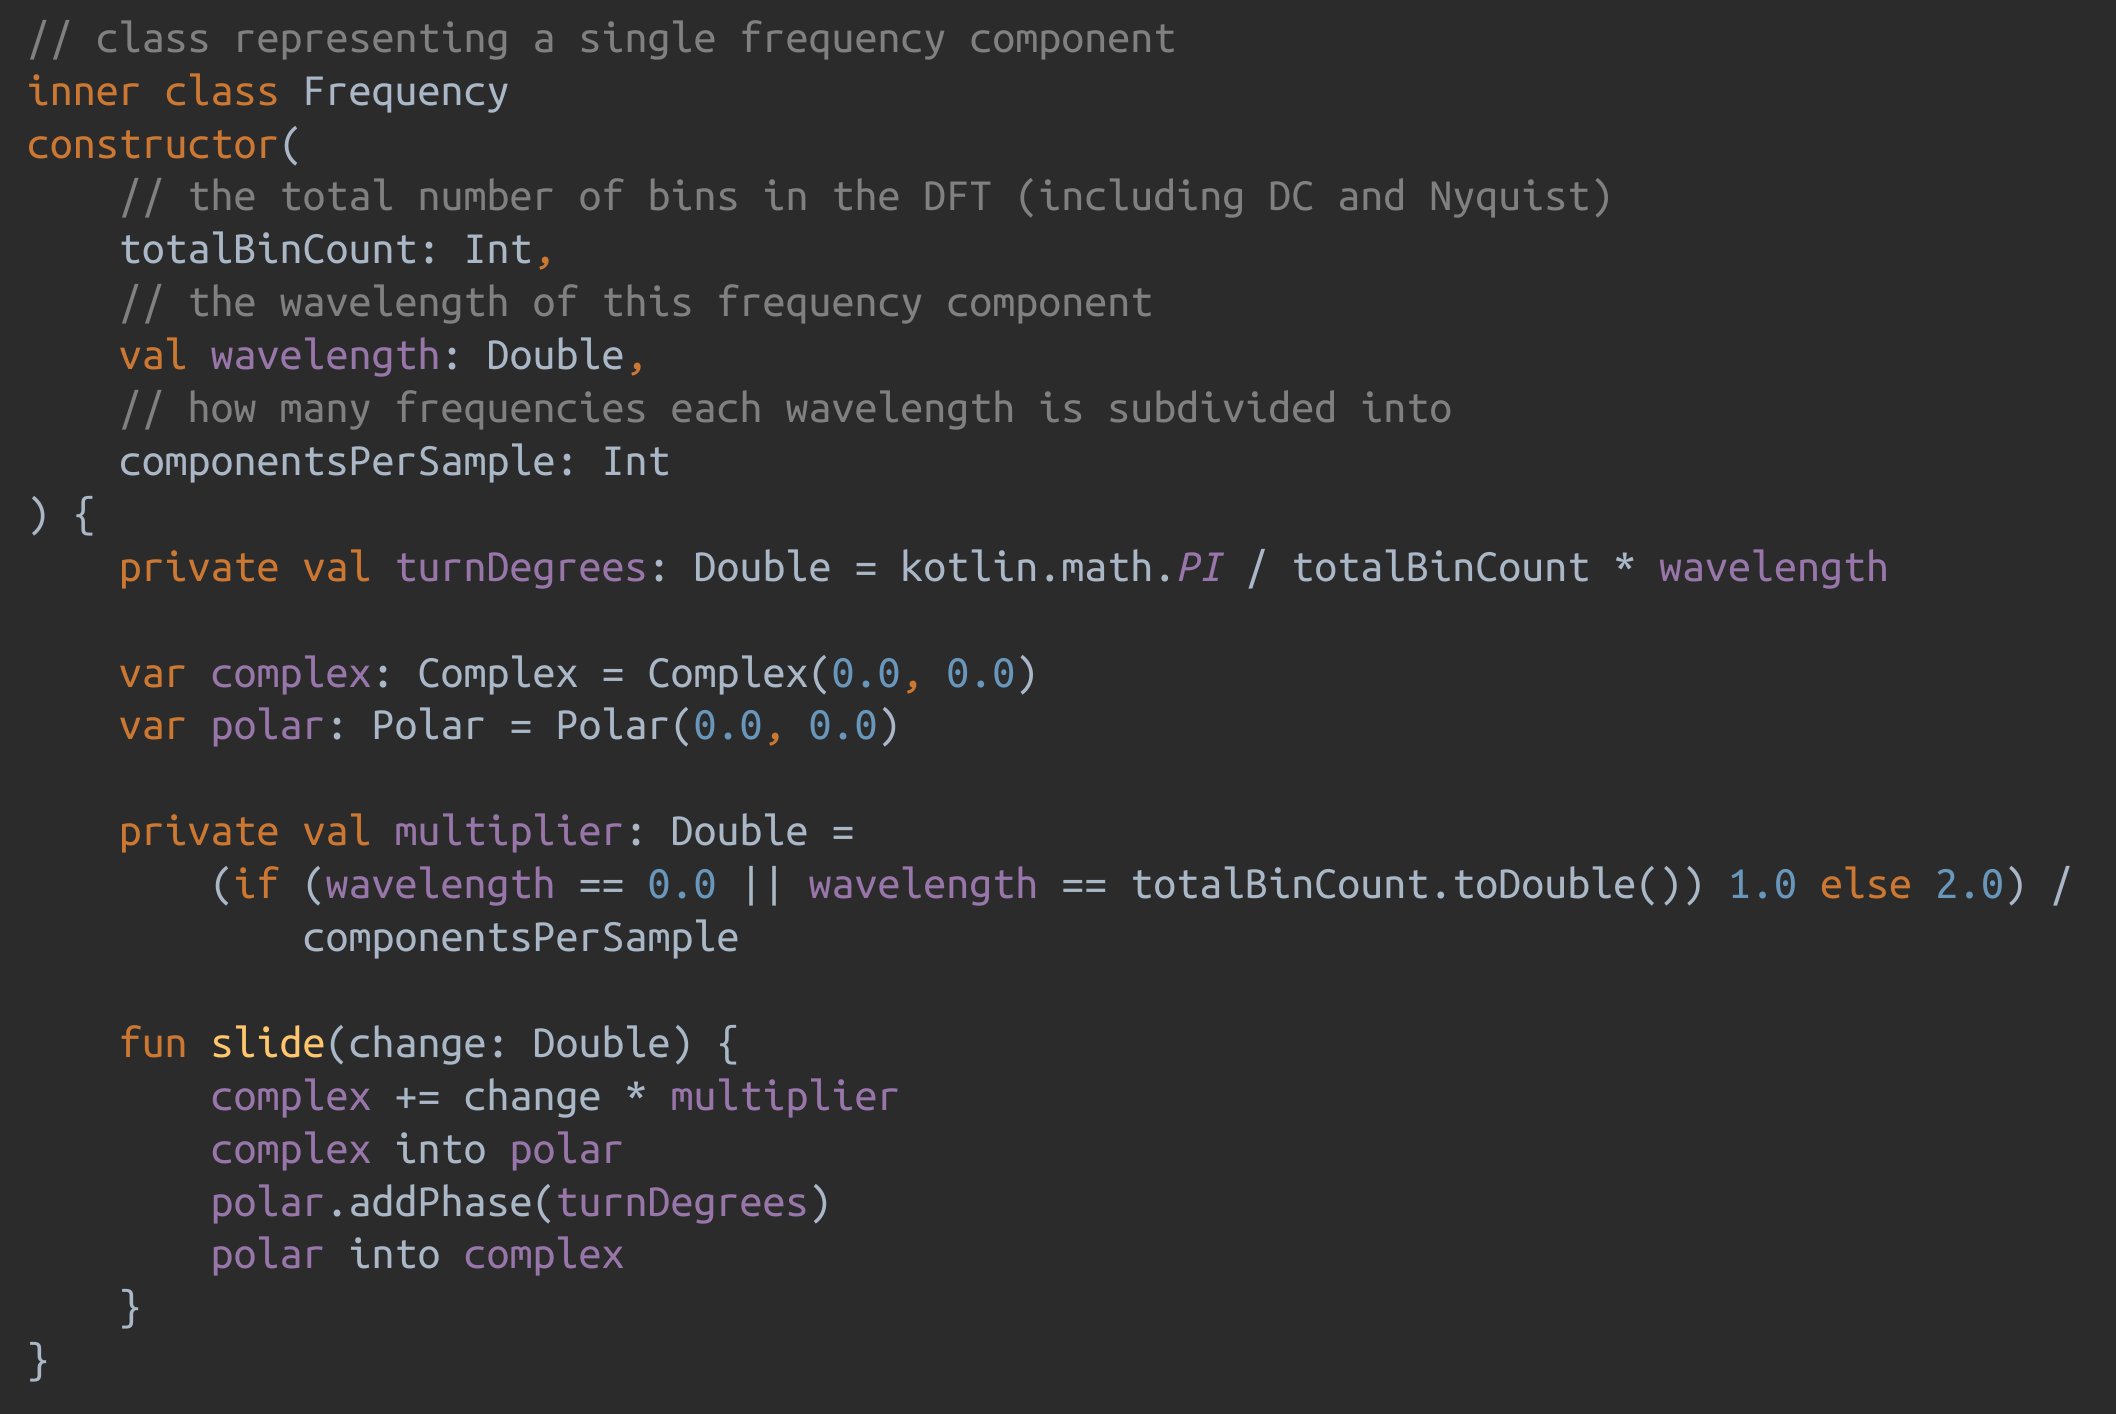
\includegraphics[width=0.9\textwidth]{code-innerClassFrequency.png}
  \caption{}
  \label{fig:innerClassFrequency}
\end{figure}

\texttt{Polar} and \texttt{Complex} are two data classes that represent a complex number in different forms. The two of them make use of a feature of Kotlin that I find rather appealing: infix functions. Both have an \texttt{into} function that converts the imaginary number from one representation into another. By using these \texttt{into} methods, we avoid recreating the objects when the imaginary number is changed from one representation to another in the \texttt{slide} function of the inner \texttt{Frequency} class, making the algorithm more efficient.

\begin{figure}[h!]
  \centering
  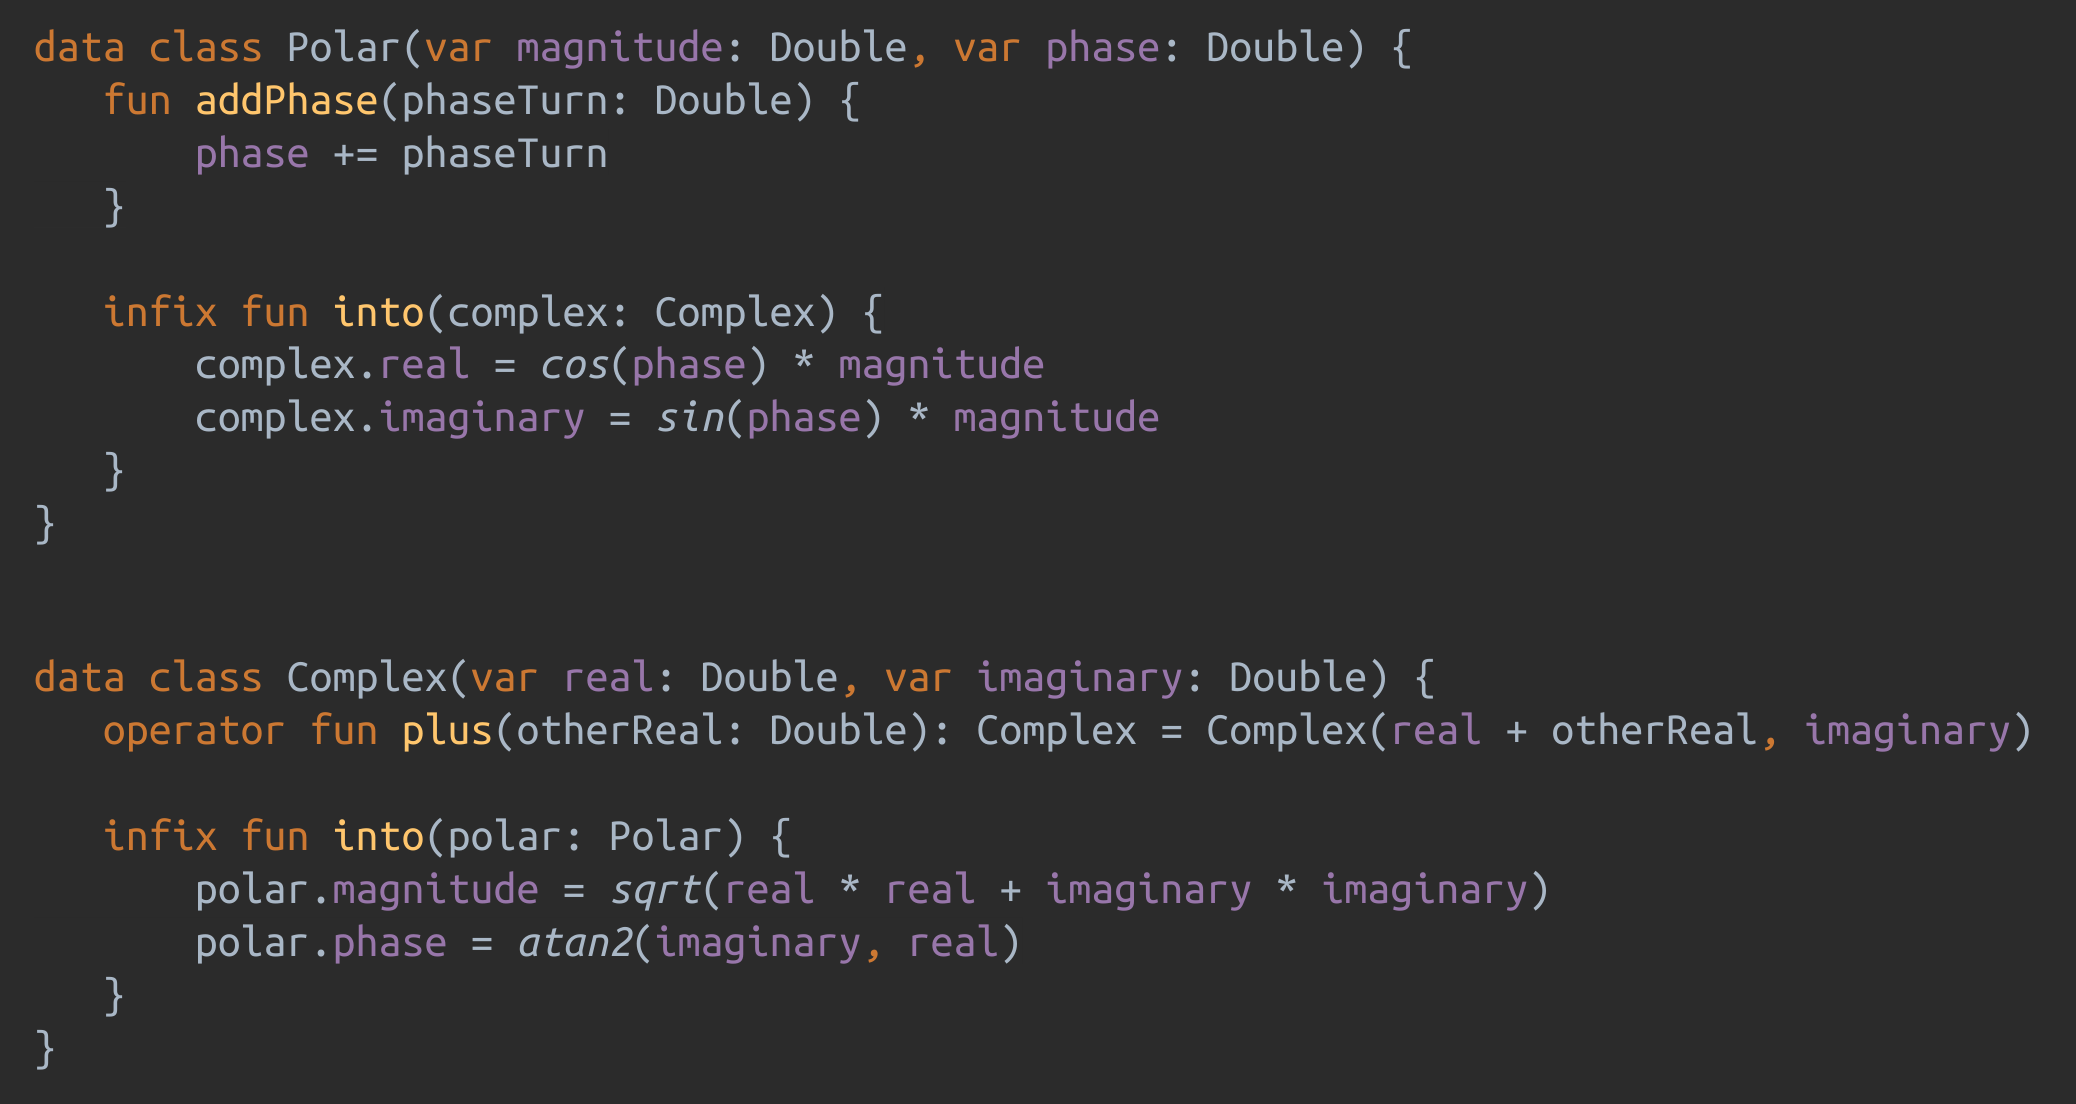
\includegraphics[width=0.9\textwidth]{code-SDFT-complex-polar.png}
  \caption{}
  \label{fig:complexPolar}
\end{figure}

\label{DFT_downsides}
Unfortunately in testing the sliding DFT proved to be inadequate for the task at hand. Although incredibly efficient (the most costly operation being the calculation of a sine and cosine) it was not able to accurately calculate the frequency of the signal. It was discovered only after some head-bashing firmly within the implementation stage that a fundamental downside of the Discrete Fourier Transform is that it is not possible to do DFT with low latency and fine frequency resolution at low frequencies.\cite{dsp_stack_dft} The frequency resolution is limited by the sampling rate, which, for a modern smartphone is somewhere in the region of 50Hz. This is insufficient to find a reasonable compromise.

By adding more frequency bins, a far higher resolution is achieved, with accuracy as far as one decimal place for the stroke rate. The downside to this is an incredibly increase in latency, with stroke rate persisting for up to half a minute (!) after device movement has ceased. Since the limiting factor is the sampling frequency, this would be a possible solution. And, with careful handling, a \texttt{SensorDirectChannel} can be accessed on Android that provides sensor sampling frequencies in excess of 500Hz, more than ten times as frequent as the smartphone's native sampling rate. However, this significantly increases power consumption for the device, both due to the increased accelerometer sampling rate and due to the increased overhead for processing more samples per second as well as the memory that would be required to store an adequately sized buffer for the readings.

As such, it was time to return back to the drawing board and a new solution was proposed.

\subsection{\texttt{Autocorrelator.kt}}

The \texttt{Autocorrelator} class provides utility methods for scoring the input readings according to their autocorrelation.

\begin{figure}[h!]
  \centering
  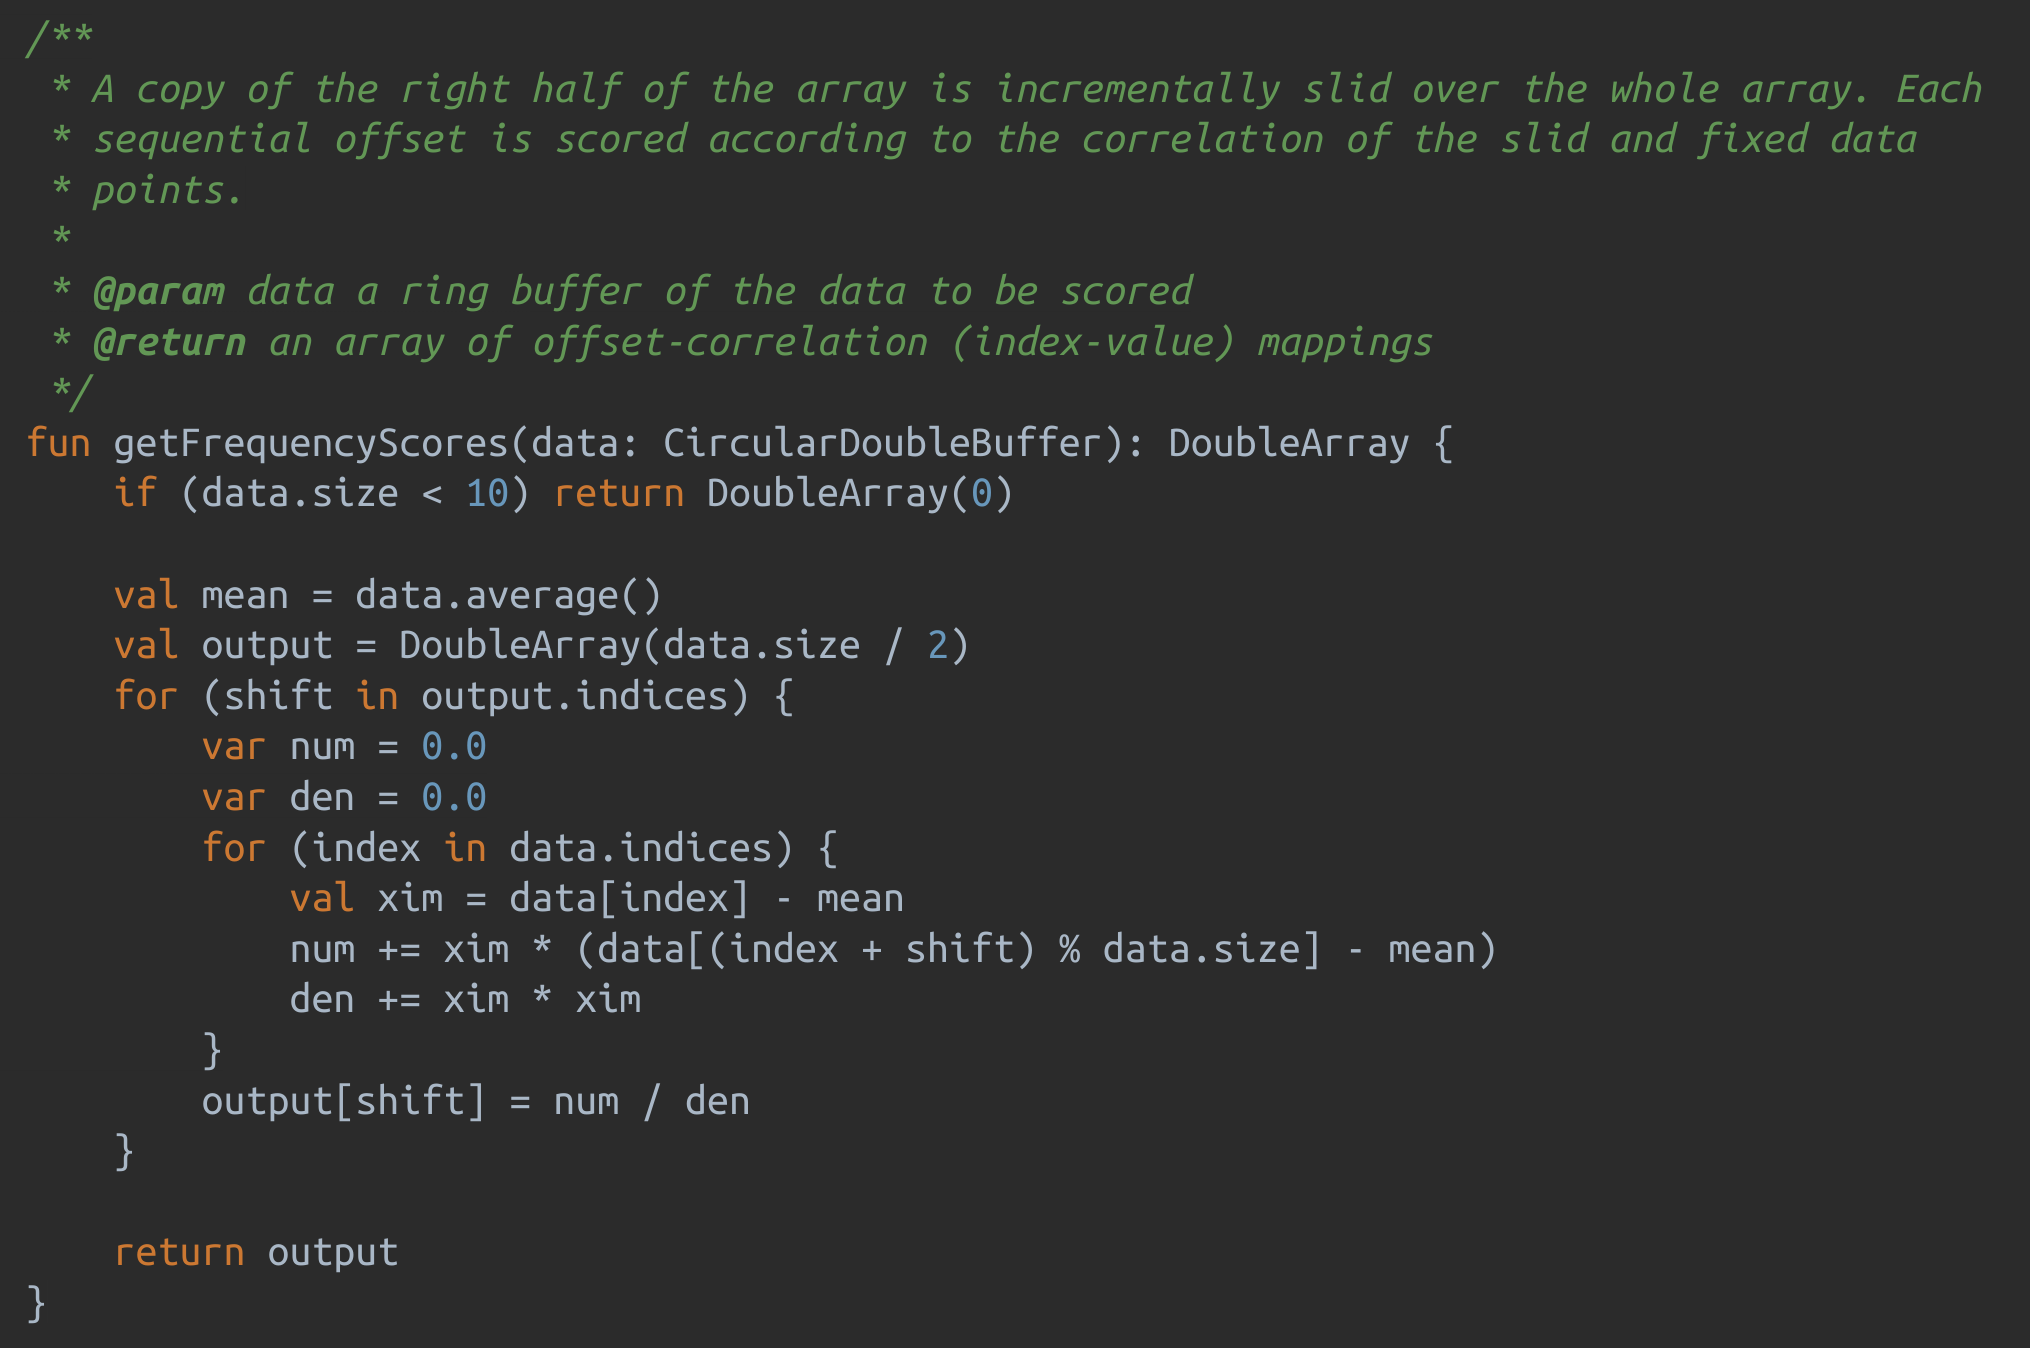
\includegraphics[width=1.0\textwidth]{code-autocorrelator-getFrequencyScores.png}
  \caption{}
  \label{fig:getFrequencyScores}
\end{figure}

The method \texttt{getFrequencyScores(data)} shown in figure \ref{fig:getFrequencyScores} implements the scoring algorithm described on page \pageref{par:autoCorAlgo}. In terms of the mathematical description of the algorithm, it returns a \texttt{DoubleArray} where the index is the offset $\tau$ and the value is the output of the autocorrelation function $R$. The \texttt{getFrequencyScores} method is called by the \texttt{DataProcessor} when the stroke rate is to be recalculated.

The mean is calculated using an inbuilt method provided by Kotlin's \texttt{Collection} interface.
There are $\frac{N}{2}$ possible lag values, where $N$ is the number of data points in the ring buffer.
The correlation scores are calculated for each lag, or offset, and saved into a \texttt{DoubleArray}. The \texttt{DoubleArray}'s index represents the lag, which is recorded as a number of samples, and the value is the calculated correlation for this offset. This method assumes that the sampling rate remains fairly constant for its results to be reliable, and this is the case for any decent accelerometer.


\begin{figure}[h!]
  \centering
  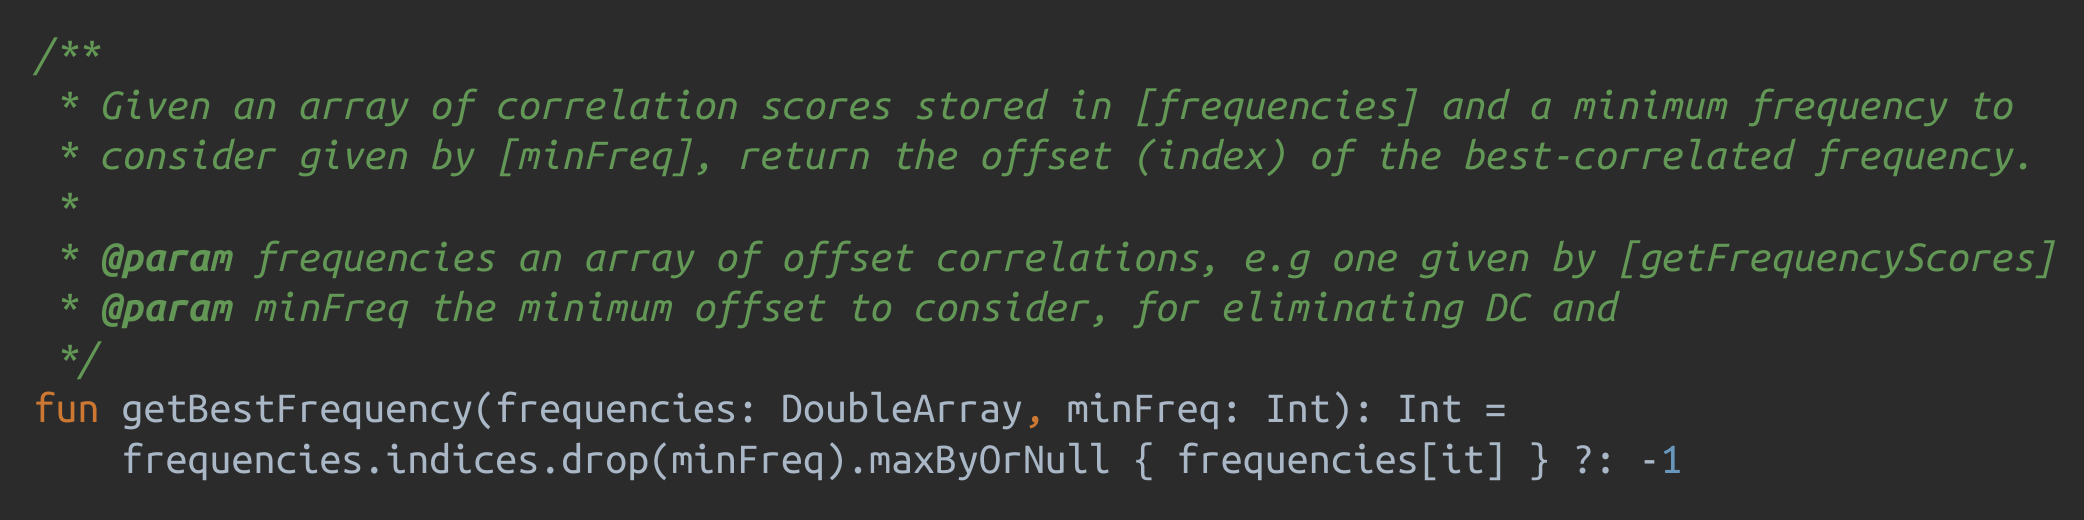
\includegraphics[width=1.0\textwidth]{code-autocorrelator-getBestFrequency.png}
  \caption{}
  \label{fig:getBestFrequency}
\end{figure}

The \texttt{getBestFrequency(correlations)} method shown in \ref{fig:getBestFrequency} selects the "best" frequency out of the provided autocorrelation array by choosing the one with the highest value. Stroke rates below a specified threshold are ignored. This is because, naturally, a tiny offset (e.g. $1$ sample) will produce a near-perfect correlation. Since very low-rate stroke detection is not necessary these frequencies can be discounted.

\subsection{\texttt{CircularDoubleBuffer.kt}}

The \texttt{CircularDoubleBuffer} class provides an implementation of a circular buffer, also known as a ring buffer, for storing \texttt{Double} values. Its primary use in the context of this application is for storing recent acceleration readings. A circular buffer was chosen for its memory efficiency and fast append operations. It fulfills the obligations of Kotlin's \texttt{Collection} interface.

\begin{figure}[h!]
  \centering
  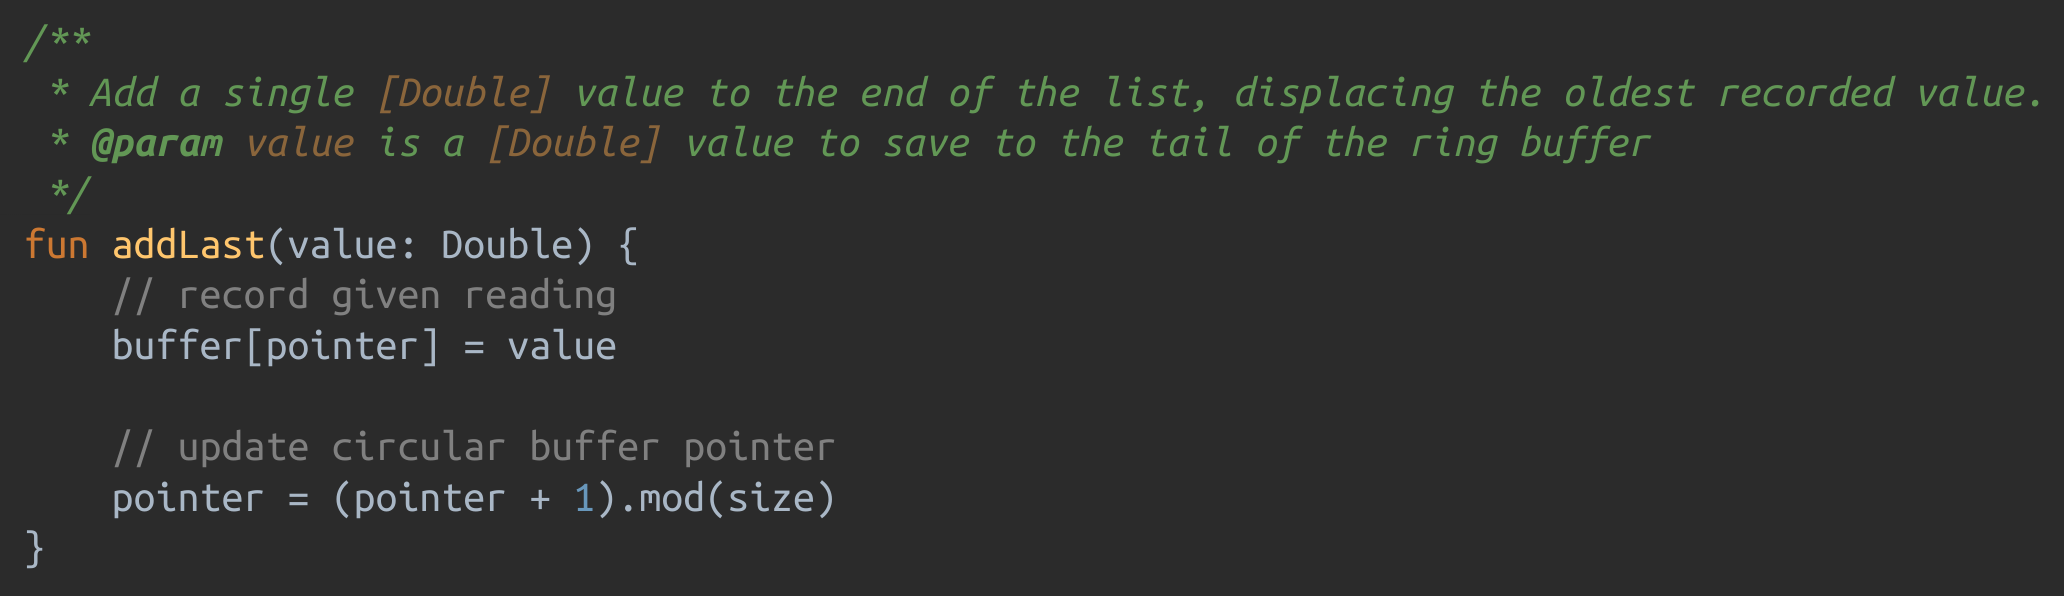
\includegraphics[width=1.0\textwidth]{code-CircularDoubleBuffer-addLast.png}
  \caption{}
  \label{fig:addLast}
\end{figure}

A single append method is necessary: \texttt{addLast(double: Double)}, the code for which is shown in figure \ref{fig:addLast}. This function stores the new value at the rear of the buffer, thus displacing (overwriting) the oldest value in the list which is no longer necessary for consideration. 

The \texttt{pointer} variable always points to the next slot to be filled, so it is incremented only after the value has been stored. The Kotlin \texttt{mod} operator is used as opposed to the infix \texttt{\%} operator, which is shorthand for \texttt{rem}. This is due to a subtlety in their functionality. The \texttt{mod} operator will always, as in mathematical modular arithmetic, return a value between $0$ and $n-1$, where $n$ is the value with respect to which modulo is taken. On the other hand, the \texttt{rem} operator can return negative values which could crash the application if it tries to access a negative index in the underlying \texttt{DoubleArray}.

\begin{figure}[h!]
  \centering
  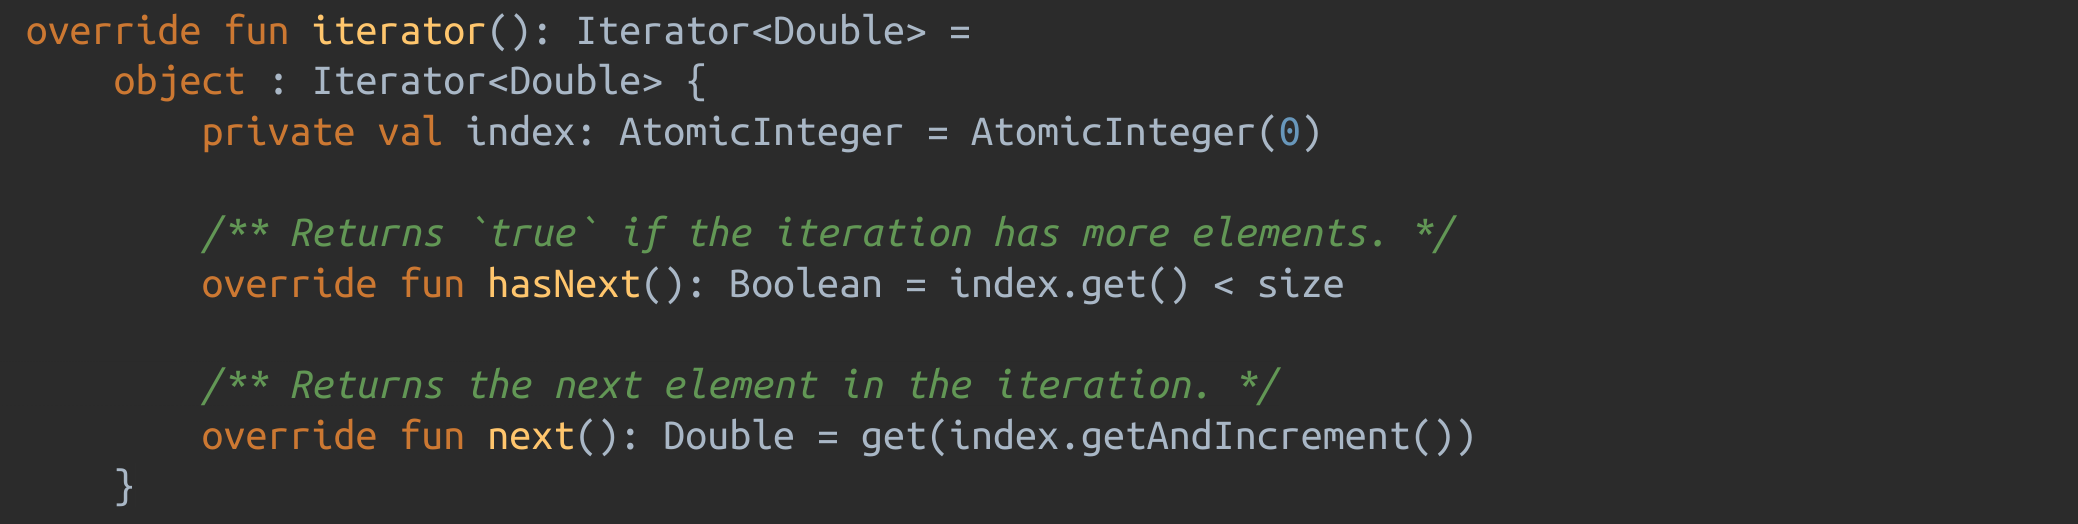
\includegraphics[width=1.0\textwidth]{code-CircularDoubleBuffer-iterator.png}
  \caption{}
  \label{fig:iterator}
\end{figure}

In addition, the \texttt{CircularDoubleBuffer} overrides the \texttt{iterator()} function of the parent \texttt{Collection} interface, as shown in figure \ref{fig:iterator}. This allows programs that use the \texttt{CircularDoubleBuffer} to iterate through the its elements as any other Kotlin list with the \texttt{for (element in circularDoubleBuffer)~\{\}} syntax. 

An \texttt{AtomicInteger} was used instead of the normal \texttt{Int} class for thread-safe operations in a multithreaded context. This allows the \texttt{CircularDoubleBuffer} to be used from separate parts of the application without concern for concurrent access exceptions.

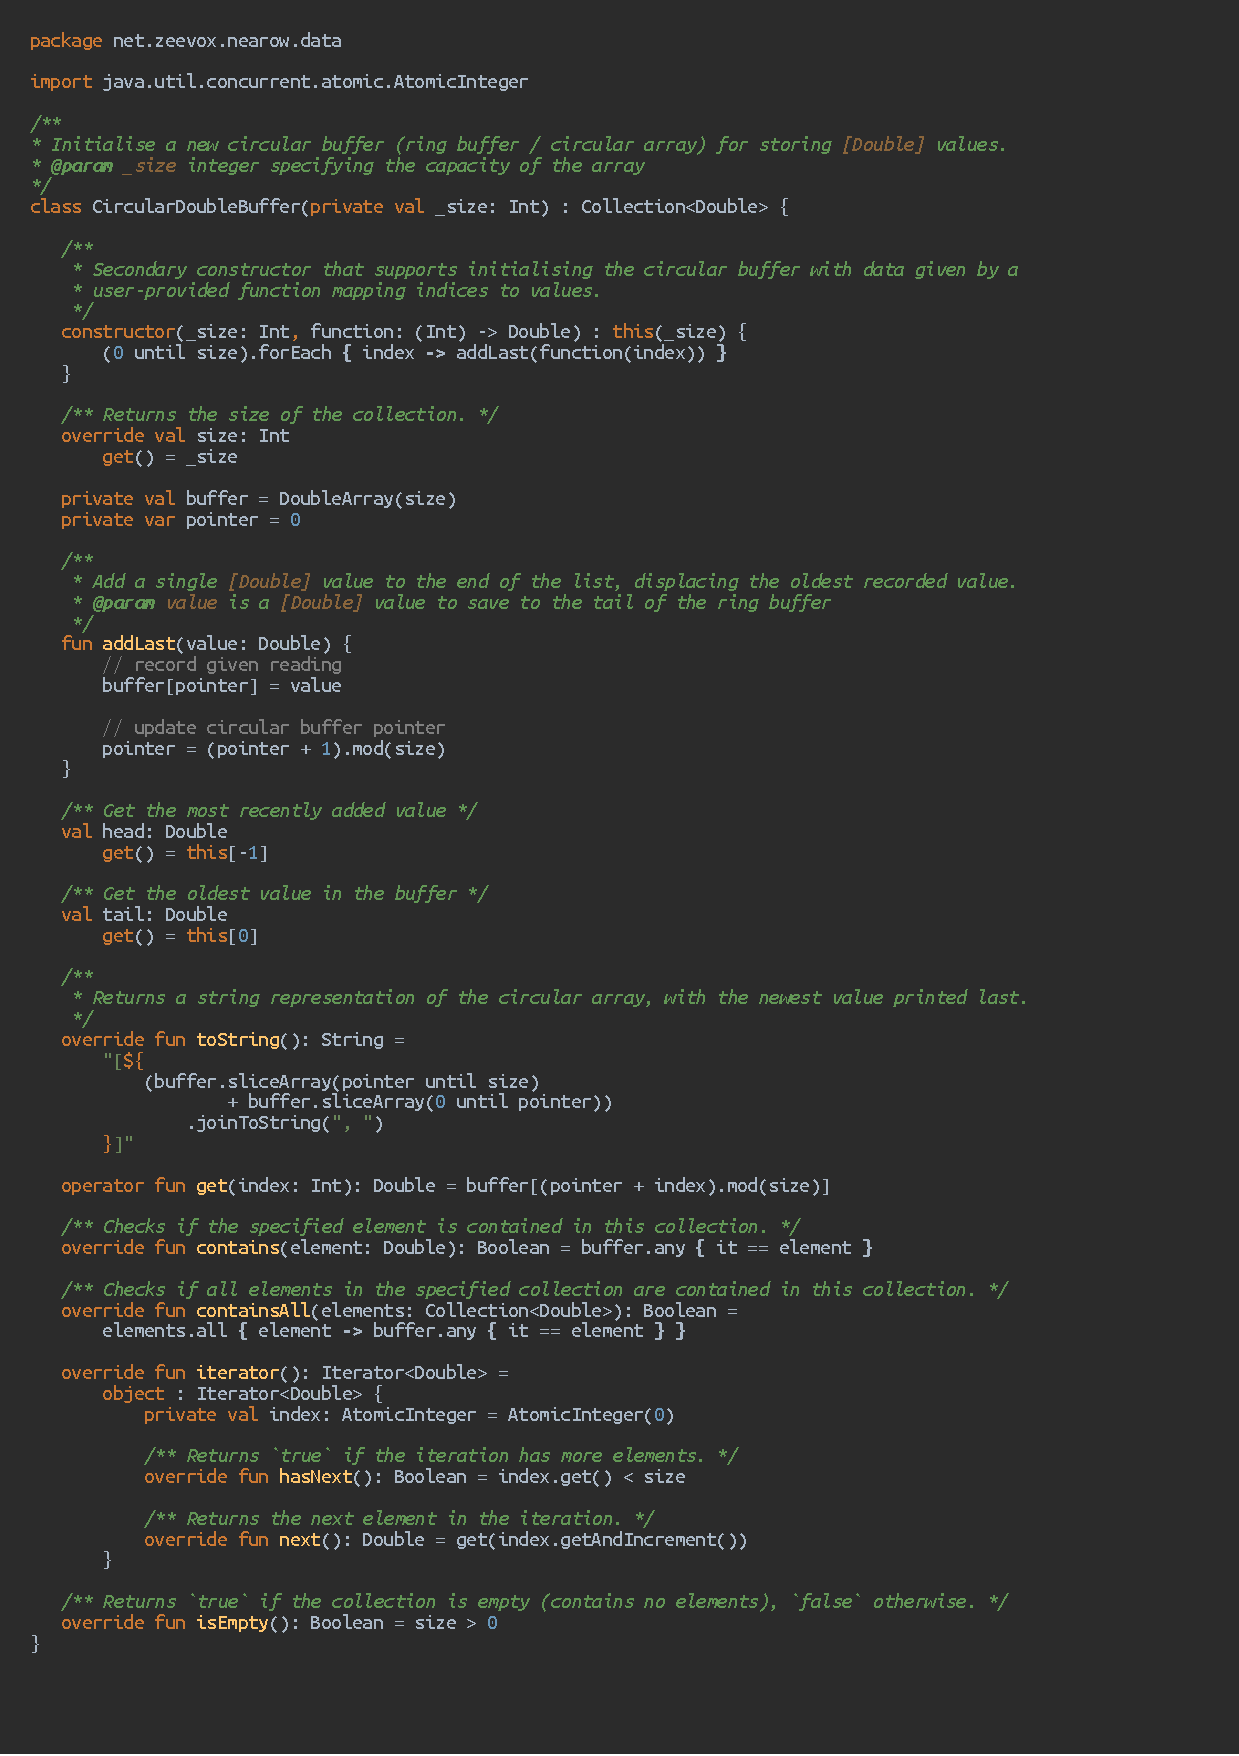
\includepdf[pages=-,pagecommand={\invisiblesection{\texttt{CircularDoubleBuffer.kt}} \label{CircularDoubleBuffer}},width=1.0\textwidth]{code/CircularDoubleBuffer.pdf}

\subsection{\texttt{DataProcessor.kt}}

The \texttt{DataProcessor} class handles the processing of incoming acceleration and location data. Accelerometer readings are smoothed and stroke rate is calculated; it tracks the total distance travelled over the course of the rowing session and informs any UI listeners of updates of any of the aforementioned metrics through callbacks. It is also responsible for persisting the calculated stroke rate, speed, and other characteristics to the application database.

The processing of the data is a computationally expensive process; since it would be unfavourable to slow down the user interface, most of the functionality of \texttt{DataProcessor} is executed on another thread. Instead of launching a full-on separate thread, we can use a functionality built into Kotlin called coroutines. 

The Kotlin team defines coroutines as "lightweight threads". They are in essence tasks that can be executed by an actual thread. Kotlin coroutine jobs can be paused and resumed, passed between different actual threads and allow for easy handling of asynchronous execution. The context of the coroutine includes a coroutine dispatcher that determines what thread the corresponding coroutine uses for its execution.\cite{kotlin_dispatchers}

\begin{figure}[h!]
  \centering
  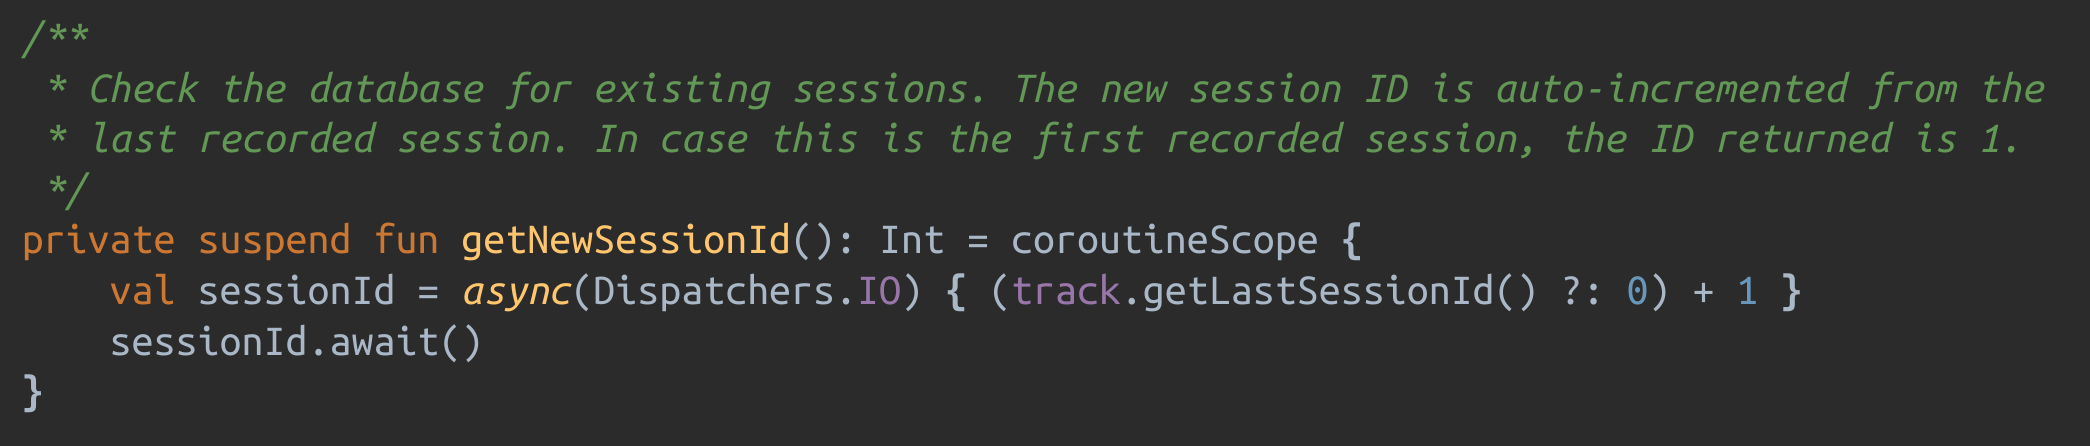
\includegraphics[width=1.0\textwidth]{code-dataProcessor-getSessionId.png}
  \caption{}
  \label{fig:dataProcessorGetSessionId}
\end{figure}

For example, the \texttt{getNewSessionId} function shown in figure \ref{fig:dataProcessorGetSessionId} gets the next sequentially availabe session ID. \texttt{Dispatchers.IO} is passed as an argument to the \texttt{async} function to specify that this command should be run on the applications I/O thread, as this function requires a SQL database query.

\begin{figure}[h!]
  \centering
  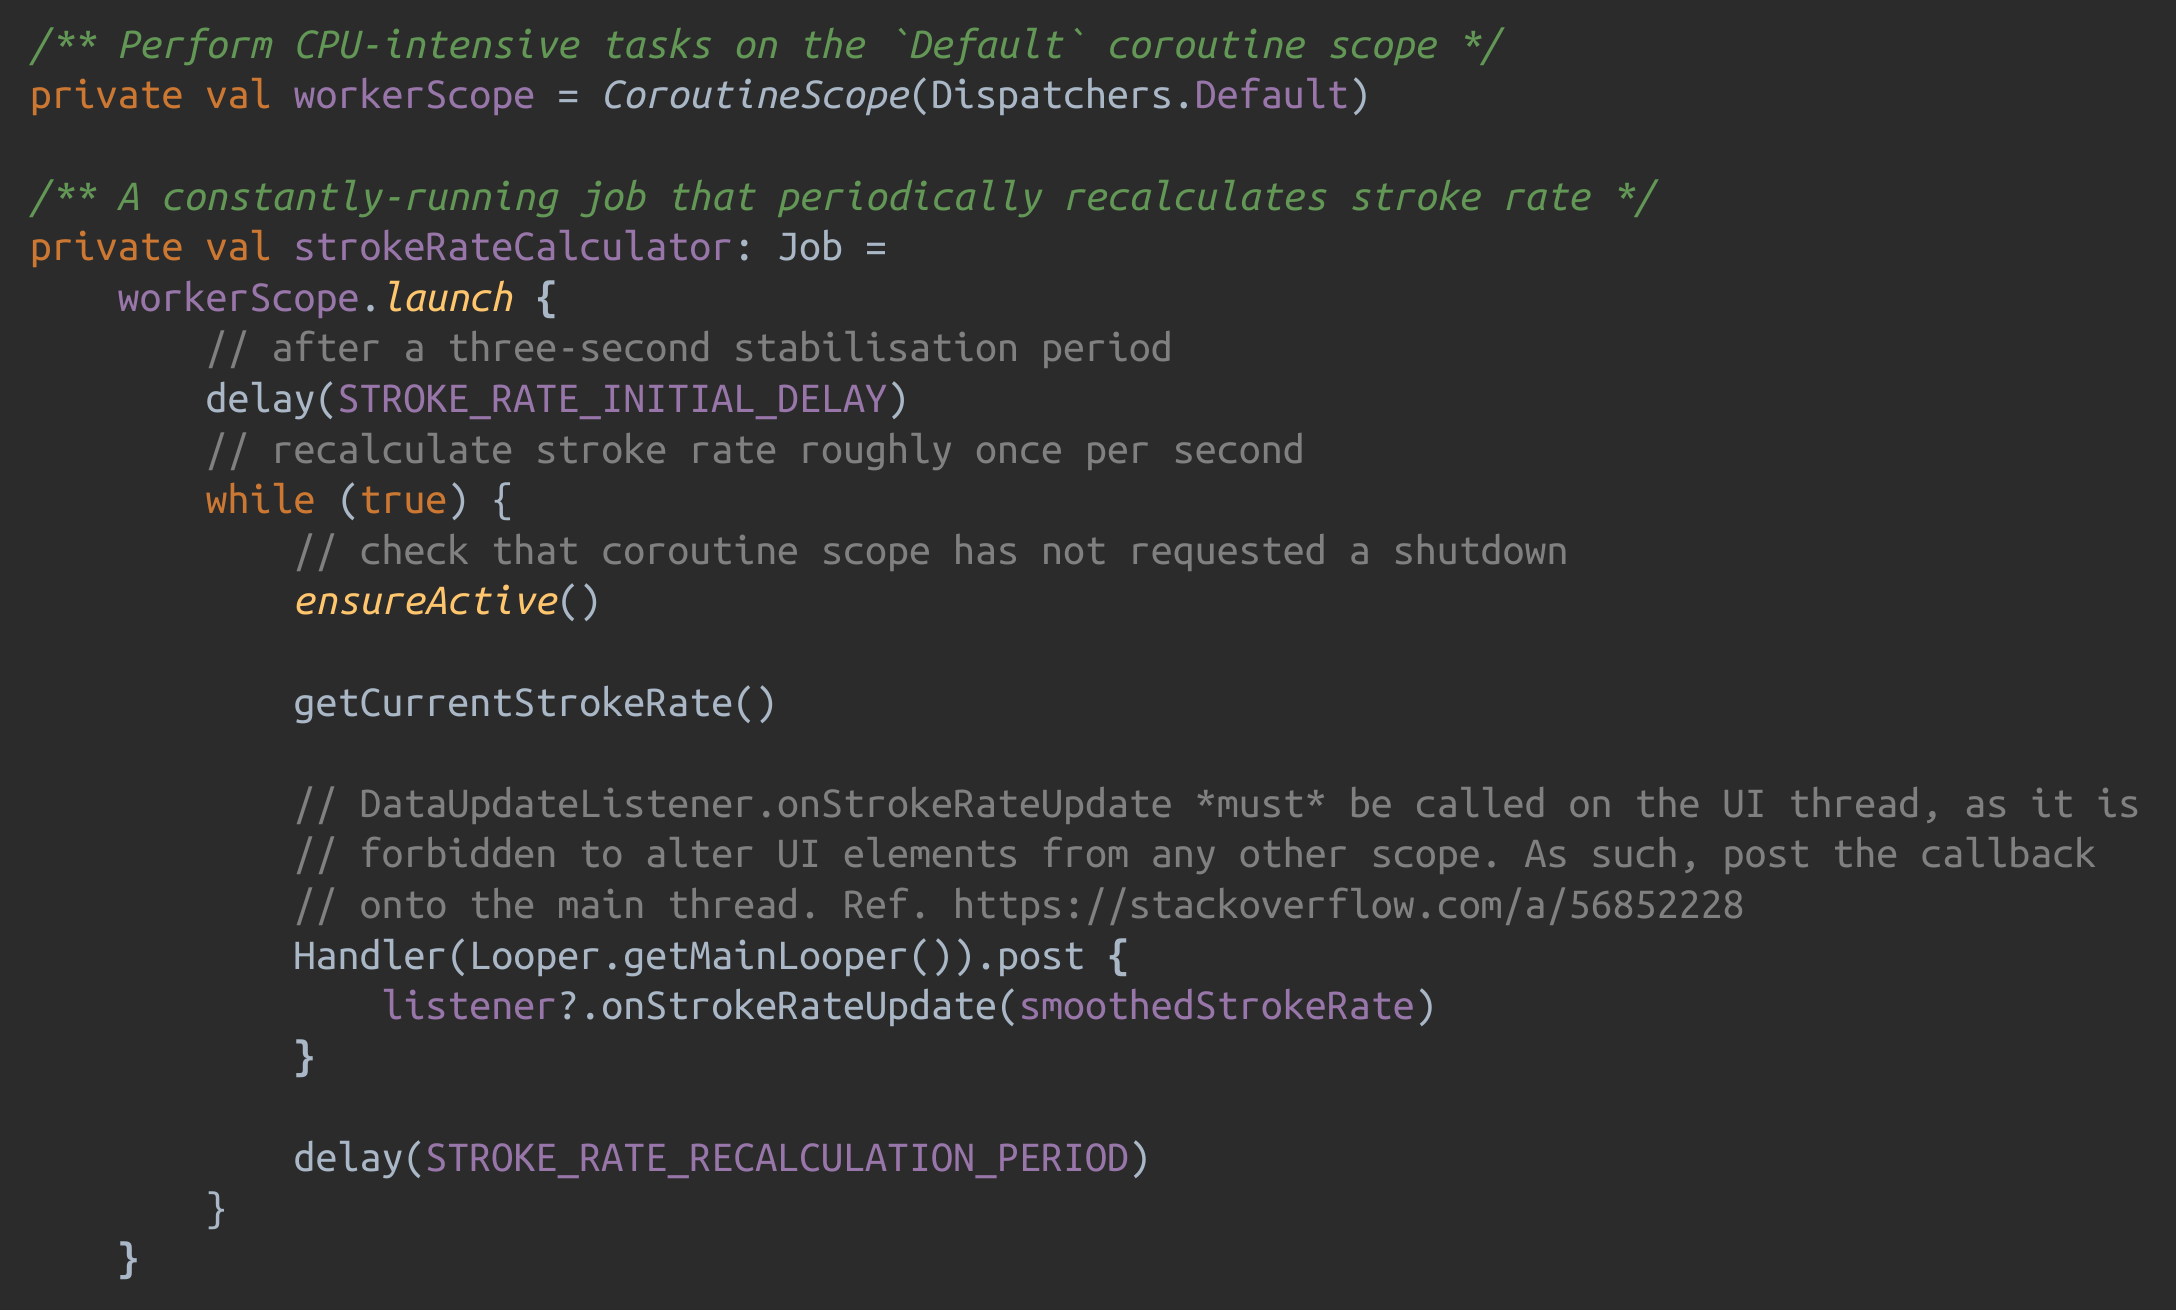
\includegraphics[width=0.9\textwidth]{code-dataProcessor-strokeRateCalculator.png}
  \caption{}
  \label{fig:strokeRateCalculator}
\end{figure}

The stroke rate is calculated by an infinitely-running coroutine job that executes on the \texttt{Default} coroutine scope, i.e. a worker non-UI thread. The code for this task is shown in figure \ref{fig:strokeRateCalculator}. 

A call to the coroutine-provided function \texttt{ensureActive} checks that the associated coroutine scope is still being used. This way, if an unhandled exception is encountered on the main thread this infinite job would still terminate despite no explicit call to do so.

However, since the stroke rate is being calculated in a worker scope, the callback to inform the listener of an updated stroke rate value has to be posted to the main thread before it can be executed. This is because Android UI elements are protected in that they cannot be modified by code running on anything but the main UI thread.

The companion object of the \texttt{DataProcessor} sets various configurable compile-time constants. In theory these could be exposed to the user, but the average rower has no need to configure any of the parameters shown. Most of these numbers were either determined empirically through testing or by calculation.

Let me draw your attention to the \texttt{ACCEL\_BUFFER\_SECONDS} quantity that specifies how large of a buffer to store with acceleration readings. This was chosen to be $10$\si{\second}. By Nyquist's theorem, frequencies with a wavelength of up to $5$\si{\second} can be detected. That results in a $60 \div 5 = 12$~spm minimum detection frequency. Stroke rates lower than $12$ are incredibly rare and inefficient. Perhaps only in the case of a specific drill might the stroke rate drop that low. A typical paddling stroke rate could go as low as $15$, which makes $12$ a reasonable lower bound.

\begin{figure}[h!]
  \centering
  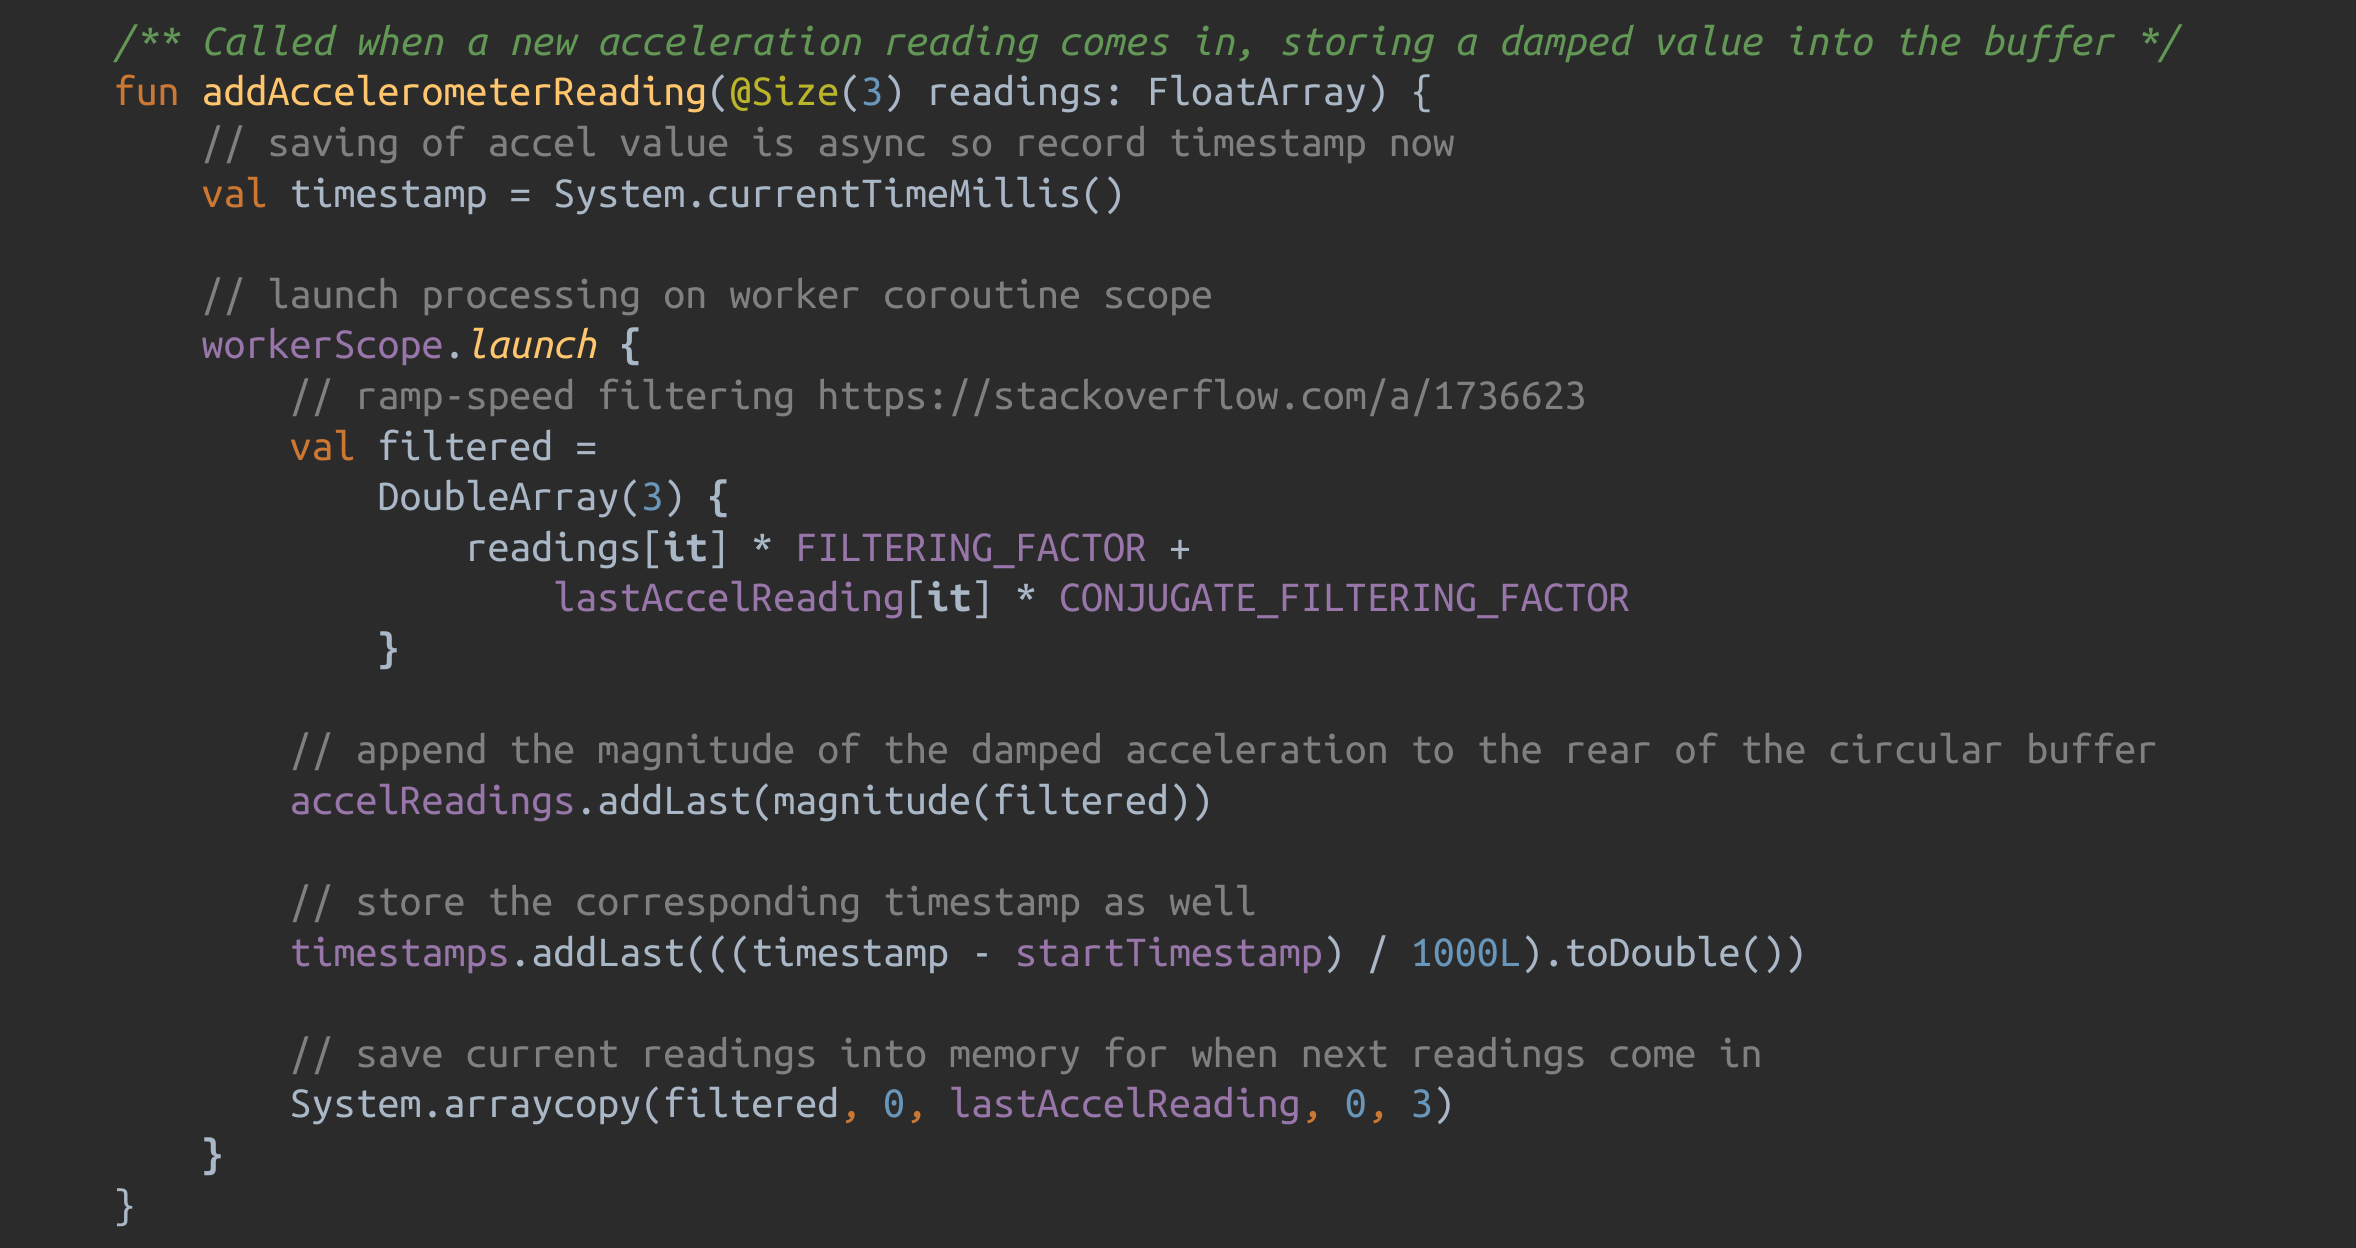
\includegraphics[width=0.9\textwidth]{code-dp-addAccelReading.png}
  \caption{}
  \label{fig:addAccelerometerReading}
\end{figure}

The companion object aslo defines the filtering factor $k = 0.1$ talked about on page \pageref{filteringFactor}. The filtering constant is put to use by the \texttt{addAccelerometerReading} method (shown in figure \ref{fig:addAccelerometerReading}), which is called when a new acceleration reading comes in. This function implements equation \ref{filterEqn} to calculate the new filtered/ramped/dampened acceleration reading, before storing its magnitude in a \texttt{CircularDoubleBuffer} of readings. 

The function also stores the corresponding timestamp of when the acceleration reading came in. This too is stored in a separate \texttt{CircularDoubleBuffer}, and is used to determinte the actual sampling rate (as opposed to the requested sampling rate) of the accelerometer. This is necessary to turn a number representing the time period of a stroke as a number of samples into a stroke rate.

Lastly, the filtered acceleration value is saved into a triple array \texttt{lastAccelReading} so that the next iteration of the ramping function can use this value to smooth the next.

\begin{figure}[h!]
  \centering
  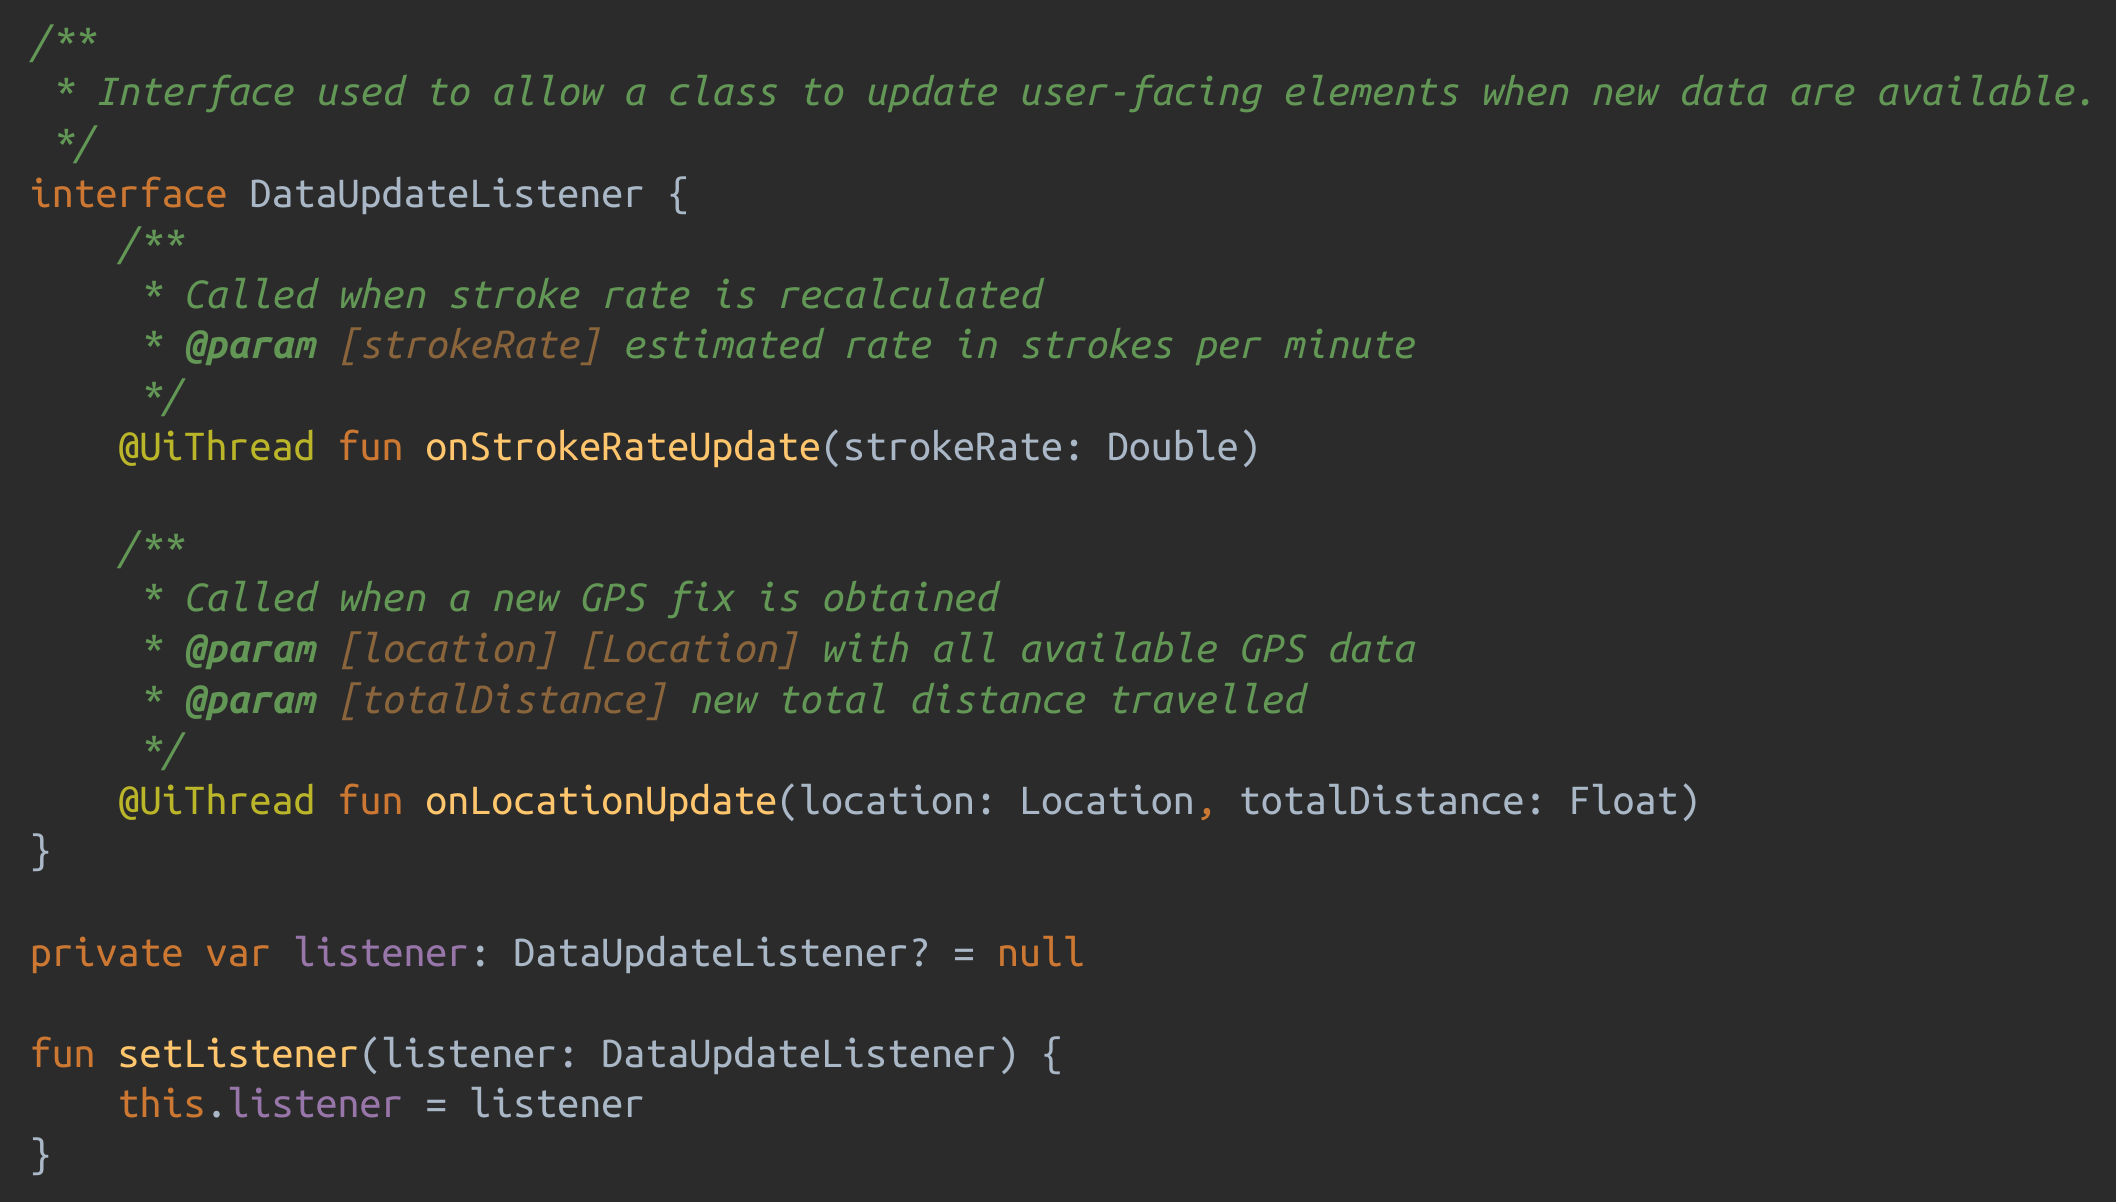
\includegraphics[width=0.9\textwidth]{code-dataProcessor-DataUpdateListener.png}
  \caption{}
  \label{fig:DataUpdateListener}
\end{figure}

The \texttt{DataProcessor} provides an \texttt{interface} that allows a UI class to listen for updates to the stroke rate or location and appropriately update the user interface. The \texttt{DataUpdateListener} interface is defined within the \texttt{DataProcessor} class, as shown in figure \ref{fig:DataUpdateListener}. The methods of the \texttt{DataUpdateListener} interface are marked with the \texttt{@UiThread} annotation so that an error message is logged if they are called from a non-UI thread.

The \texttt{listener} variable is marked as nullable (with Kotlin's typing system), since the \texttt{DataProcessor} may not always have a corresponding UI thread listening for stroke rate and location updates, or if the user interface goes out of view it will cease to listen for stroke rate updates. The \texttt{listener} variable is private to prevent other classes with access to the data processor instance from obtaining a reference to the listener. Only a setter is made available, so that a new listener can be installed (for example, for when a UI fragment is recreated).

Notable extracts of the implementation have been inserted as figures above; the full code for the \texttt{DataProcessor.kt} is displayed overleaf.

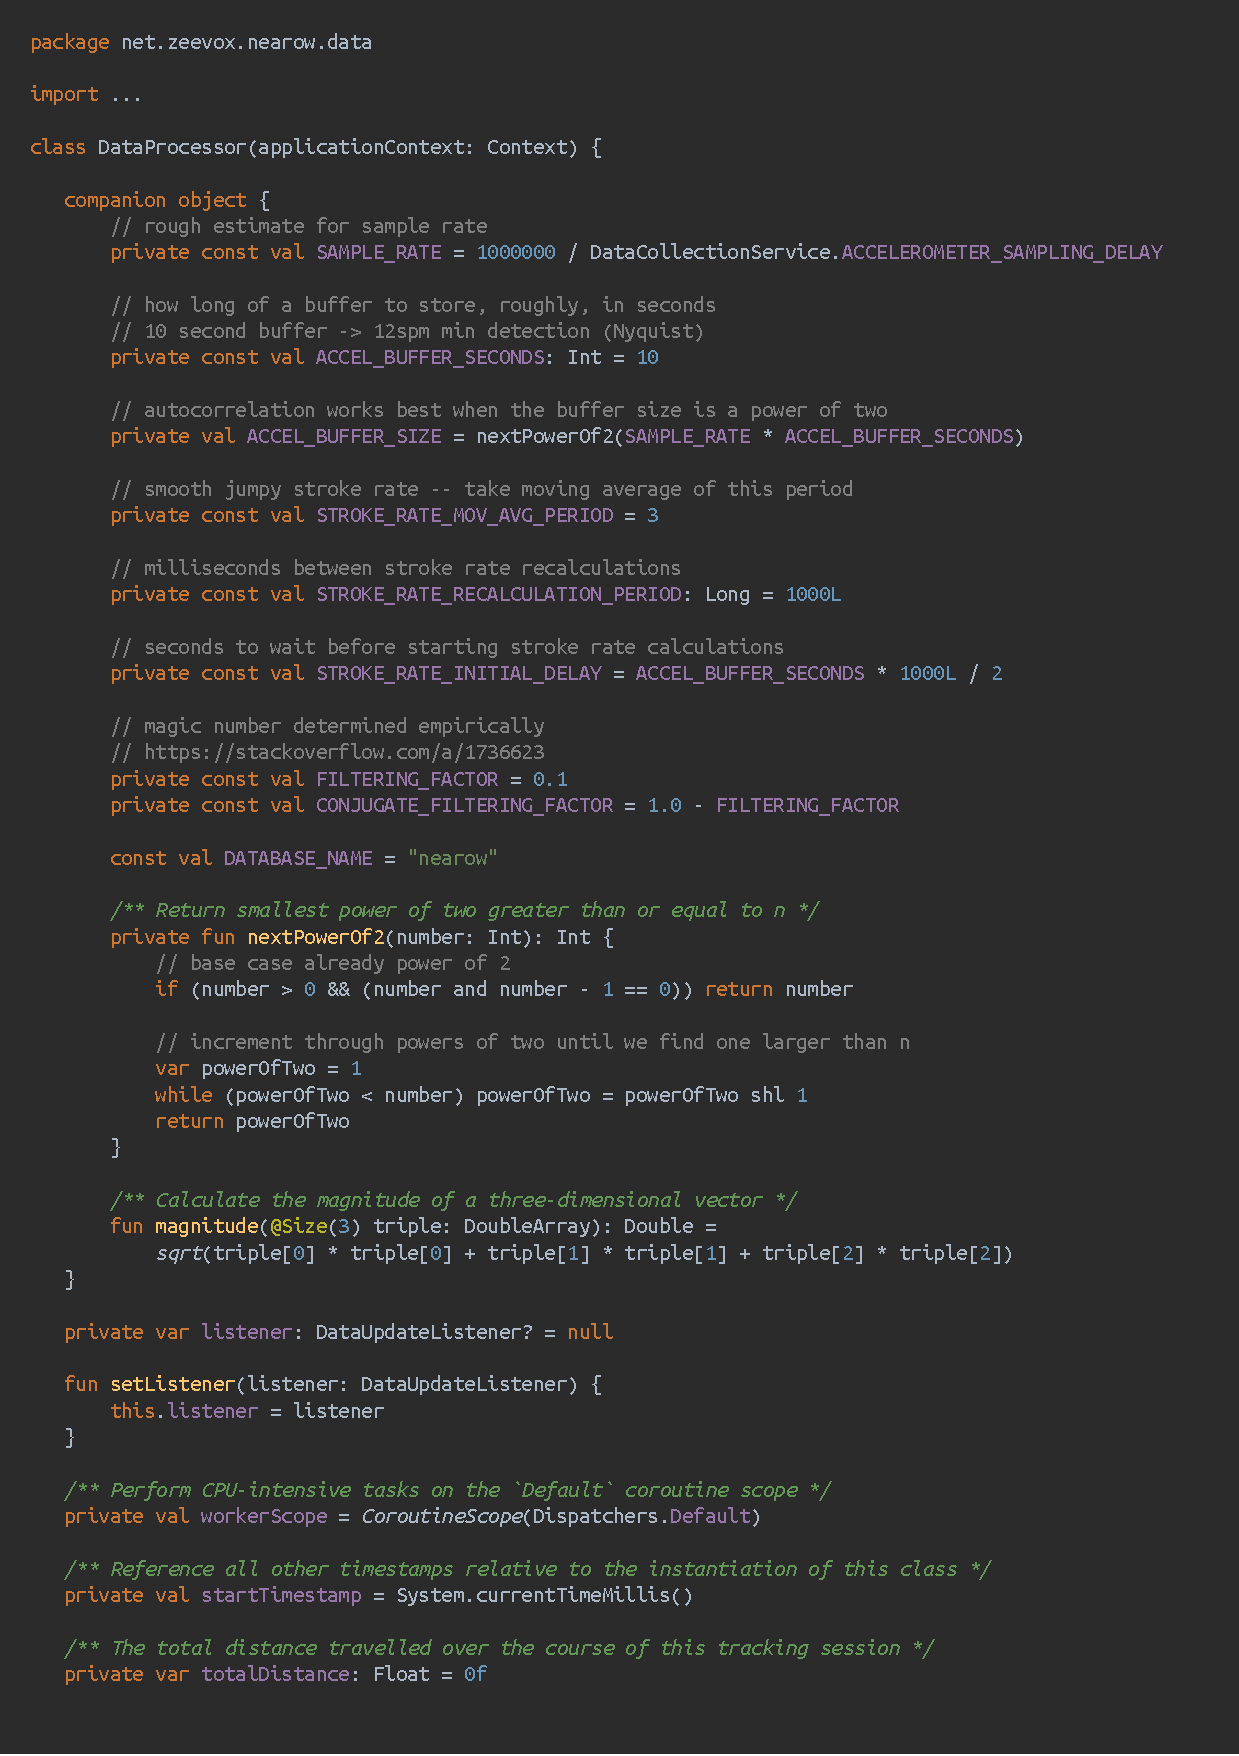
\includepdf[pages=-,pagecommand={},width=1.0\textwidth]{code/DataProcessor.pdf}

\subsection{\texttt{UnitConverter.kt}}

A utility class that converts between different units of measurement, in particular rowing-specific ones such as split and watts. All of the functions it provides are moved inside the Kotlin \texttt{companion object} since they do not require instantiation of the class itself. 

\begin{figure}[h!]
  \centering
  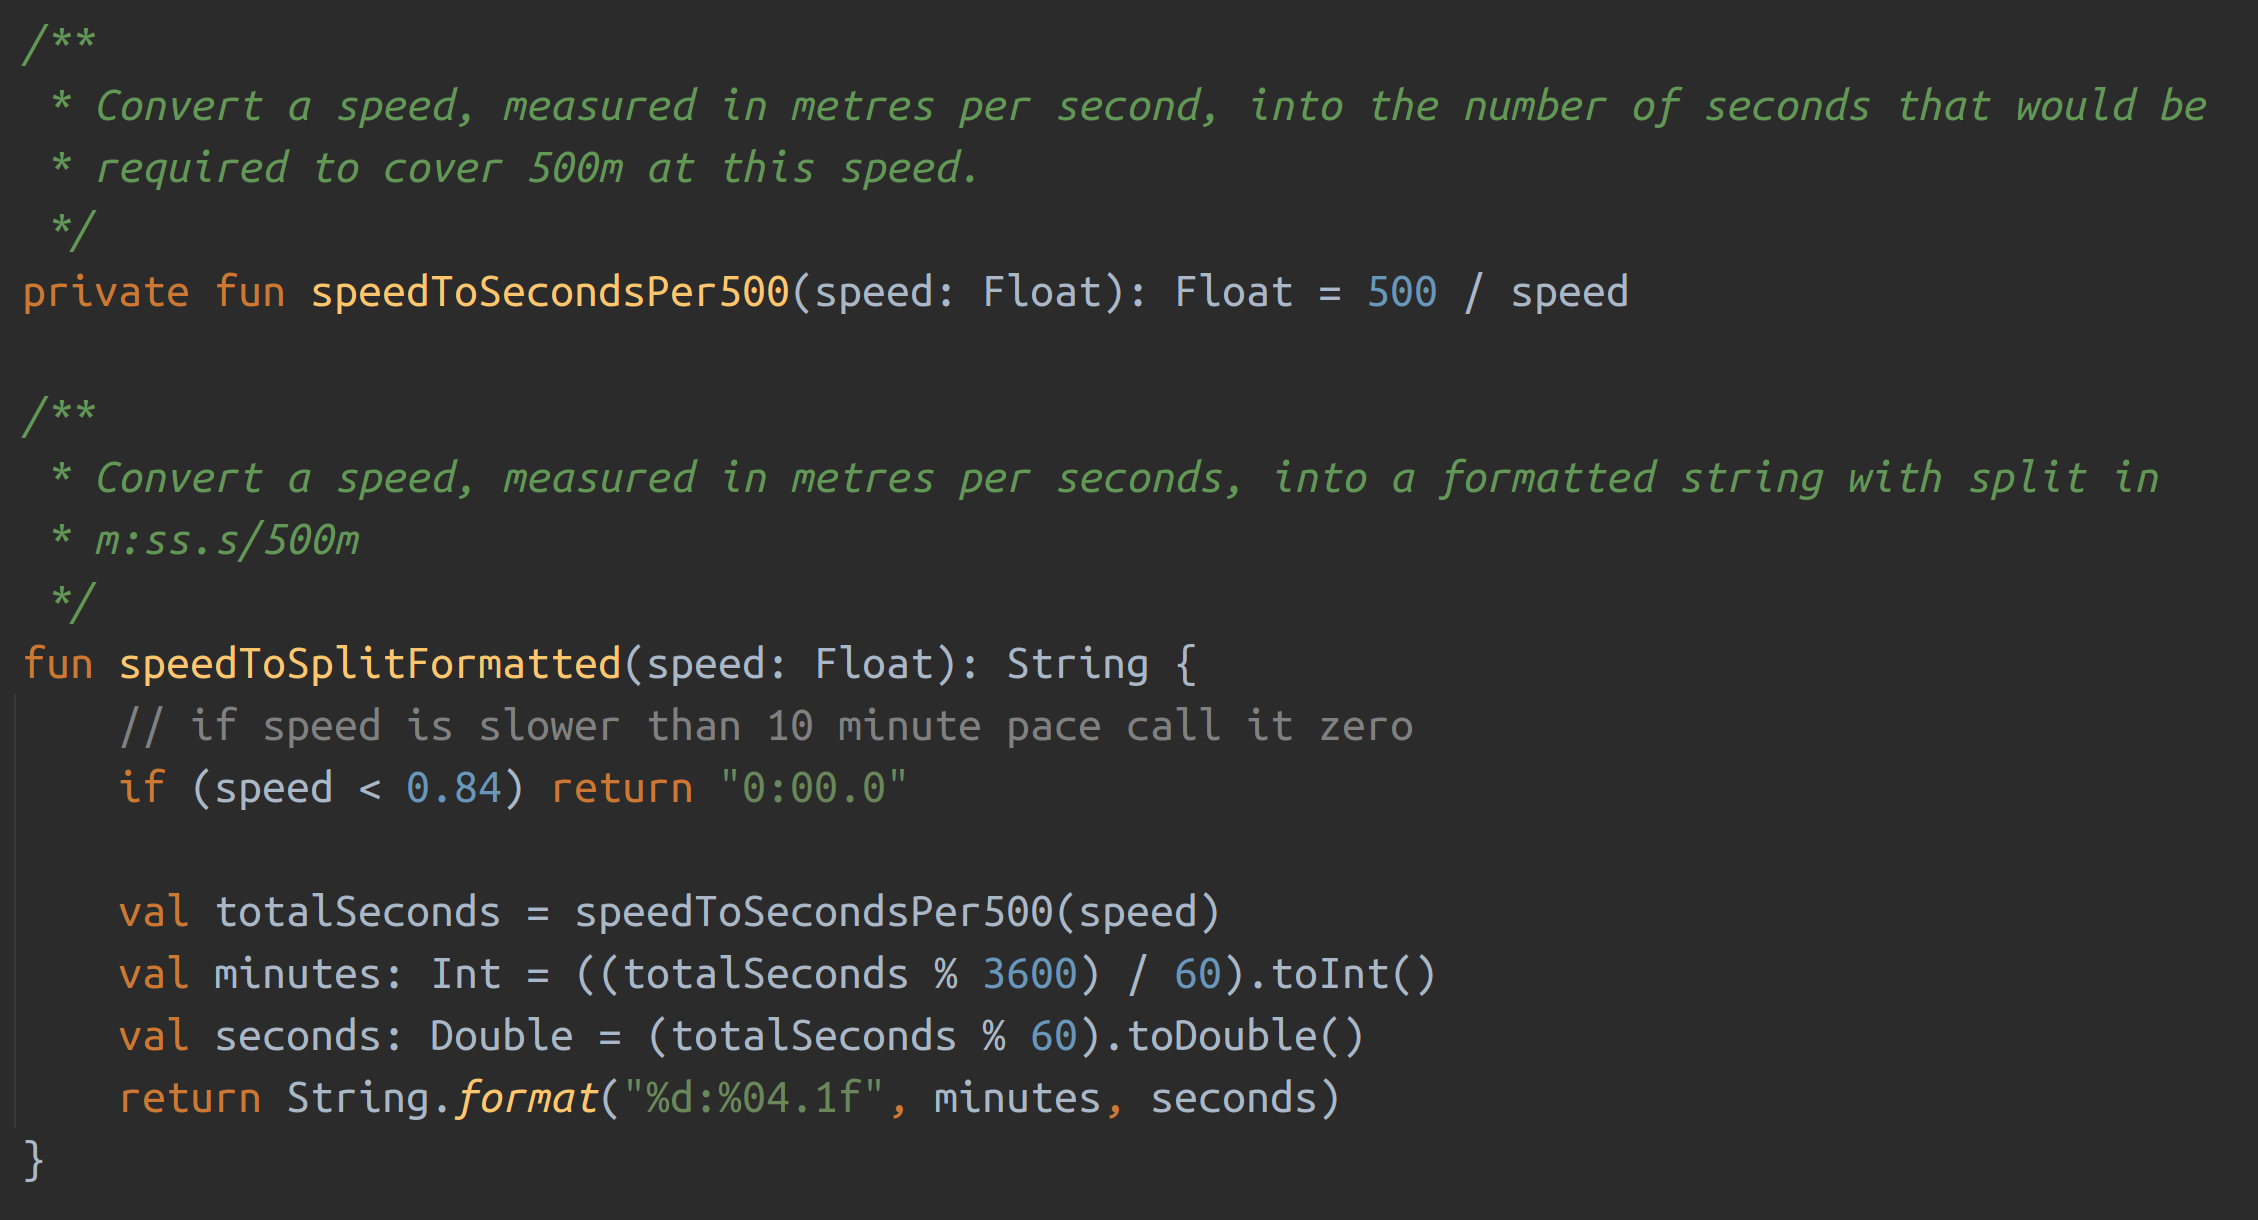
\includegraphics[width=0.9\textwidth]{code-splitformatting.png}
  \caption{Functions for converting speed into a typically formatted rowing split}
  \label{fig:splitformatting}
\end{figure}

Figure \ref{fig:splitformatting} shows the code necessary for converting speed into a rowing split. A special behaviour is implemented for that case that the speed provided is exceptionally slow (i.e. less than 10:00/500m split $\simeq 0.84$\si{\meter\per\second}), in which case the speed is considered to be $0.0$\si{\meter\per\second}. An interaction unexpected to me was the Java string formatting placeholder for a float. In order to achieve a zero-padded number of minutes with one decimal place (i.e. $3$ numerical digits), the \texttt{\%0\textbf{4}.1f} format specifier is used, since the decimal dot is counted as a numerical digit.

\begin{figure}[h!]
  \centering
  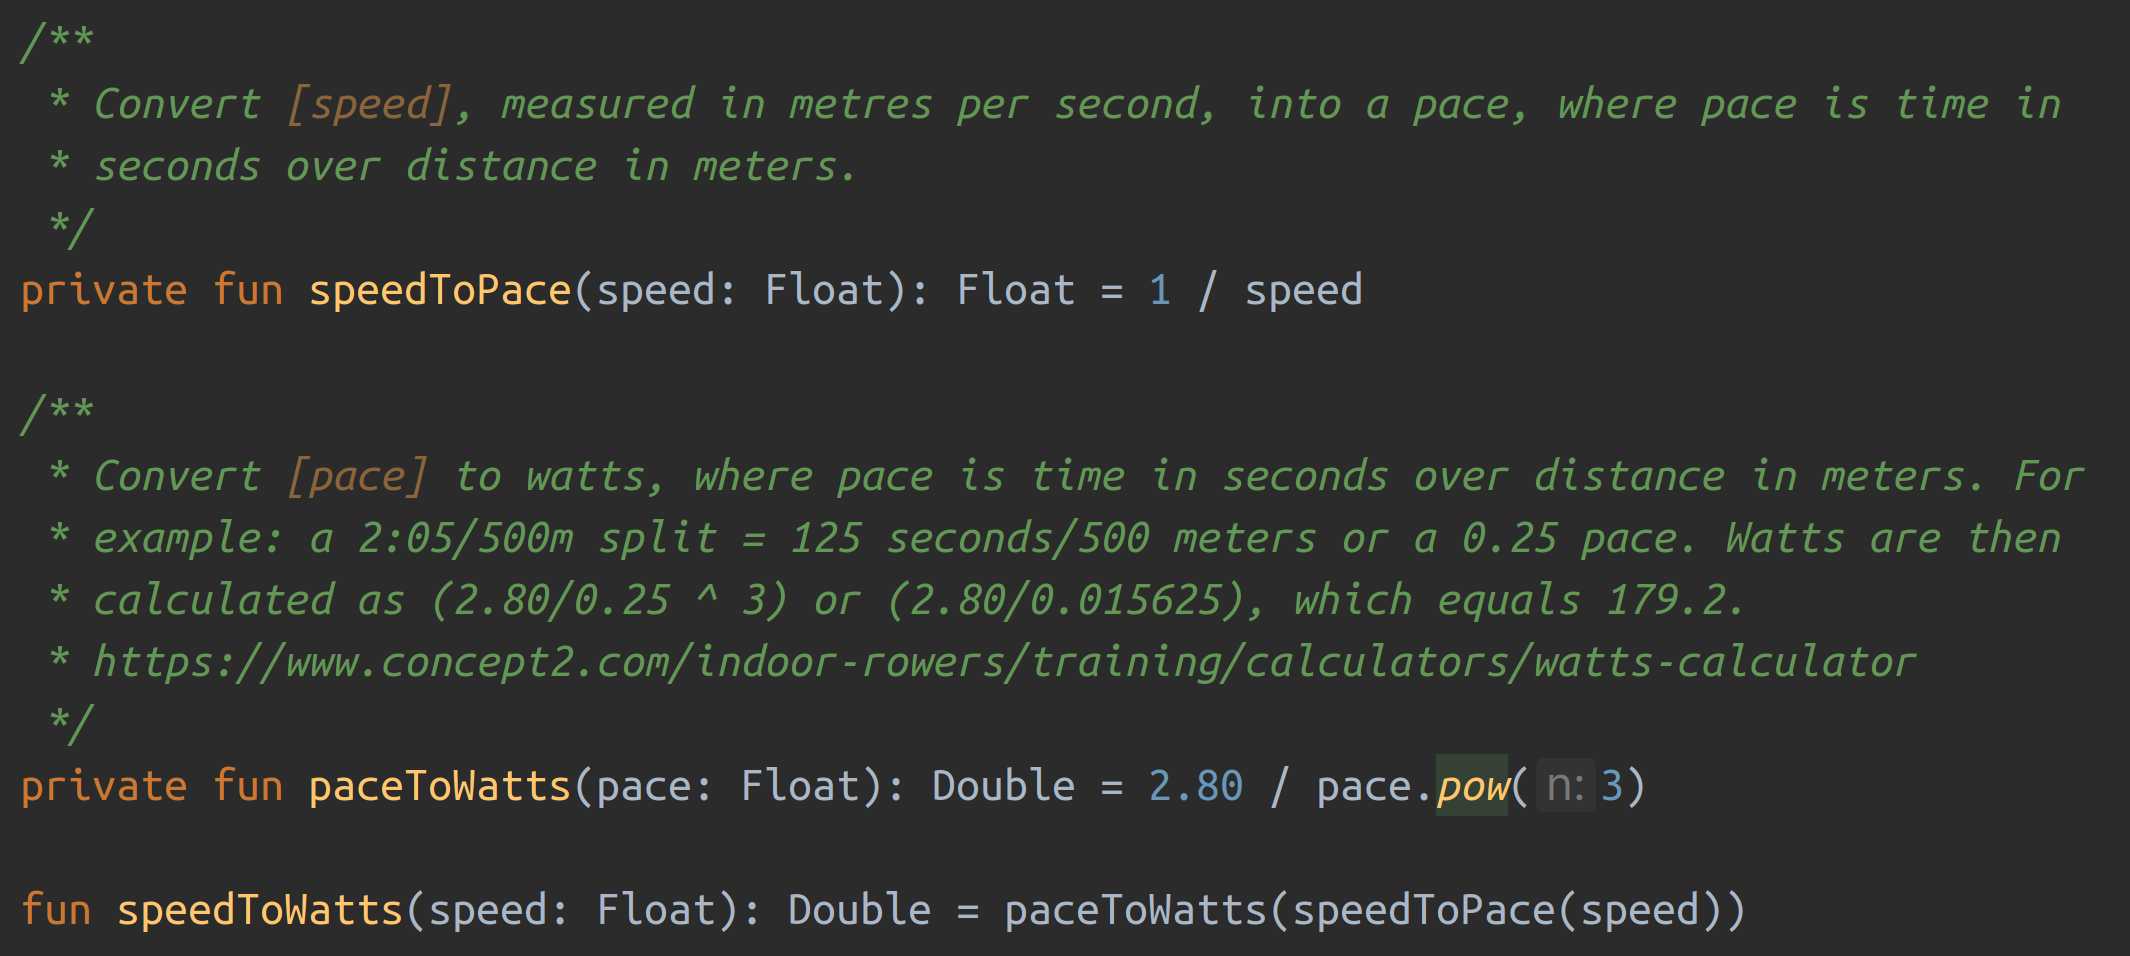
\includegraphics[width=0.9\textwidth]{code-watts.png}
  \caption{Functions for converting speed into estimated power}
  \label{fig:watts}
\end{figure}

A given speed can also be converted into an estimated power value, using a formula determined empirically by Concept2, the leading manufacturer of rowing machines.\cite{c2_p2w} The formula is:
\begin{equation}
  \frac{2.80}{\left(\frac{\text{seconds}}{500}\right)^3}
\end{equation}

\section{Data storage}

Each entity corresponds to a table in the associated Room database, and each instance of an entity represents a row of data in the corresponding table. The \texttt{TrackPoint} class is an entity. Each row in the table corresponds to a single track point, recording the timestamp of when it was taken, the stroke rate at that instance and the the geolocation. The speed of the boat, in metres per second is also recorded. This is because the Android location provider can produce a more accurate speed than simply measuring the distance between two successive track points, for example if the Doppler measurements from GNSS satellites are taken into account.

The database table is updated and queried through a \textit{data access object}, defined in \texttt{TrackDao.kt}. The \texttt{TrackDao} class is a Kotlin \texttt{interface} that defines the methods that can be used to access the database. The SQL queries used for retrieving data from and inserting data into the database are defined within annotations for each method. No function body is provided, since this is autogenerated by the Room library. The SQL queries themselves are abstracted from application classes, which can only use the functions defined within the \texttt{TrackDao} interface to access data. Note that all of the functions in this class are marked \texttt{suspend}. This is because they deal with access to secondary storage, and as such could take a long time to complete. As such they must not be executed on the main thread but inside a coroutine, preferably on the I/O thread provided by the Android framework.

The \texttt{TrackDao} interface is used by the \texttt{TrackDatabase} class, which is defined in \texttt{TrackDatabase.kt}. The \texttt{TrackDatabase} class is a Kotlin \texttt{data class} that defines the database schema. A database version number is provided for version control and back-compatibility on potential future updates to the application.

The code for the four database-related classes is shown overleaf.

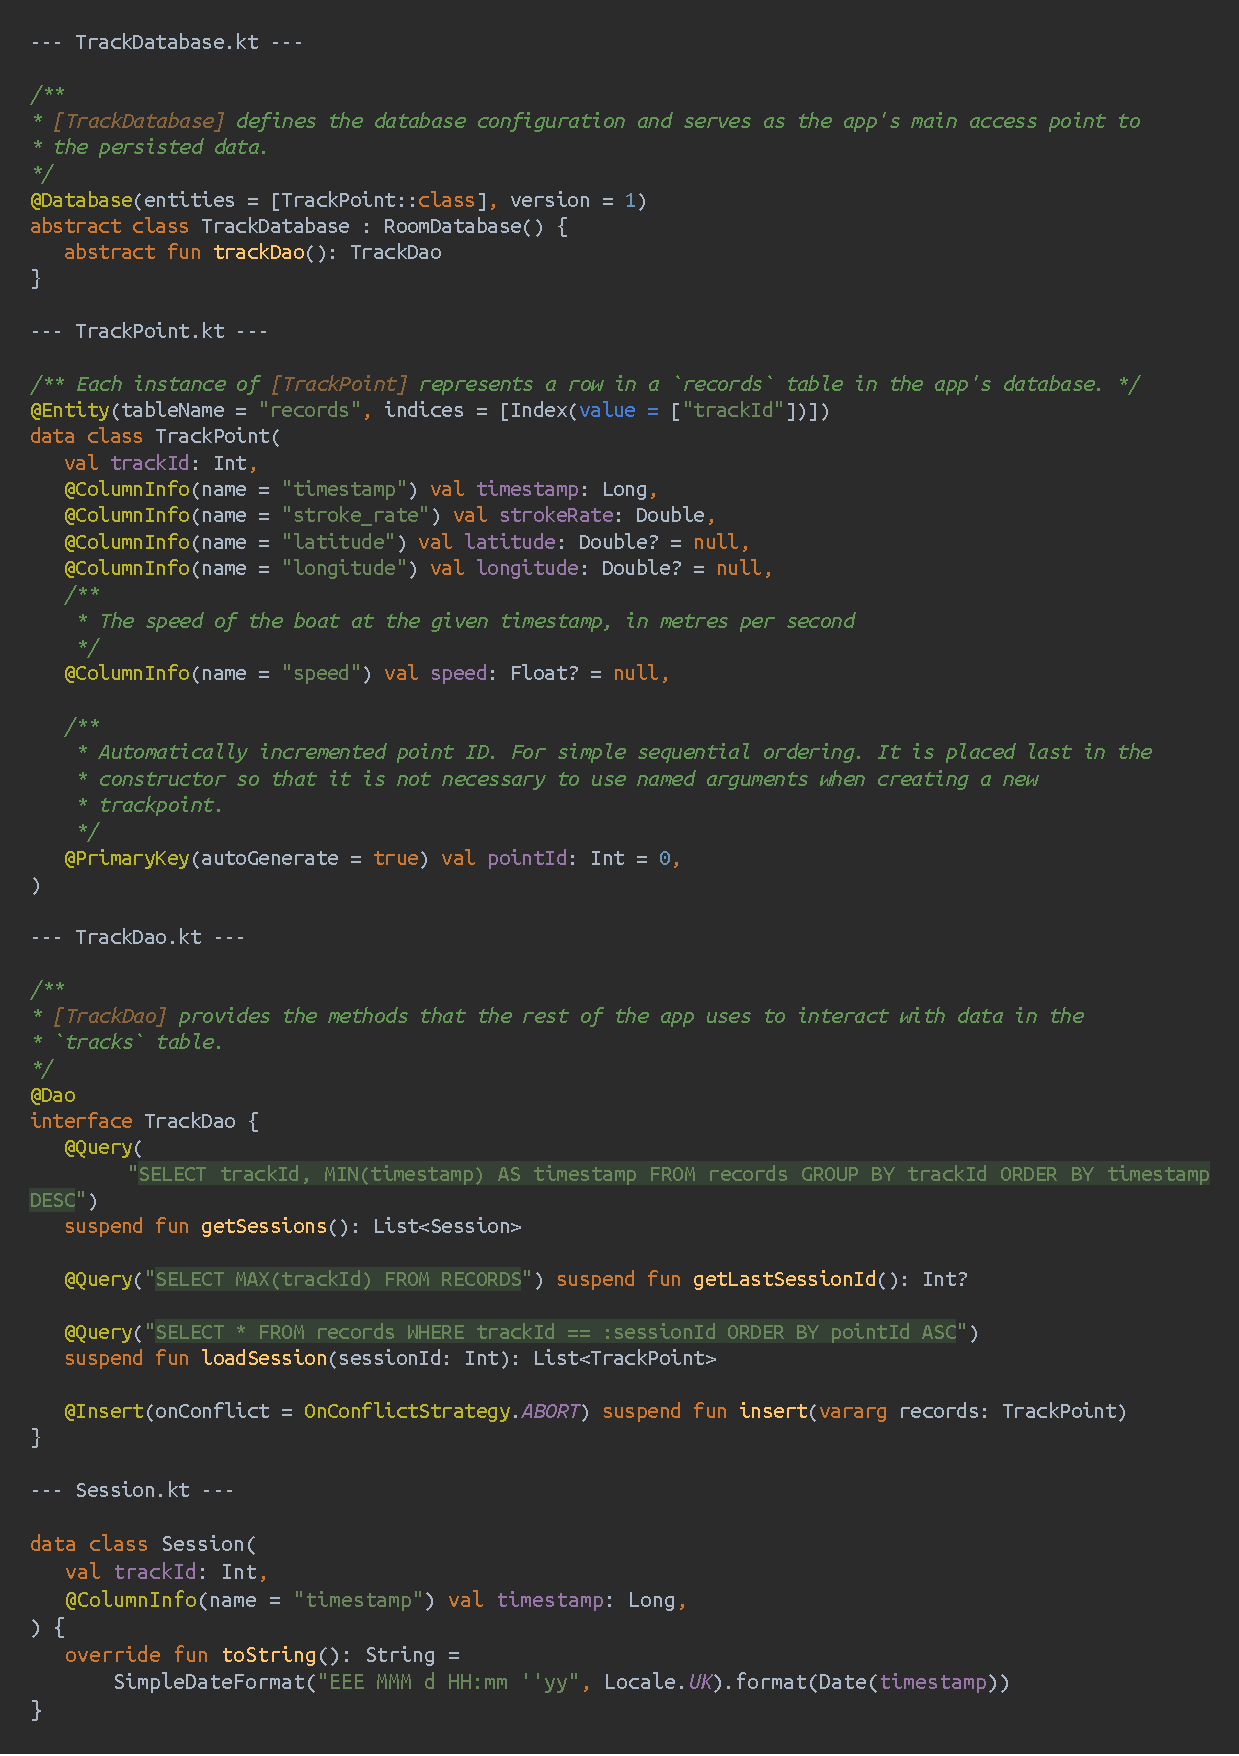
\includepdf[pages=-,pagecommand={},width=1.0\textwidth]{code/Database.pdf}

\section{File export}

The code for the \texttt{FitFileExporter} class is shown in the appendix on page \pageref{FitFileExporterStart}. Given a list of \texttt{TrackPoint} objects, representing the rows of the database, a Garmin FIT activity file is produced. It was chosen to take a list of \texttt{TrackPoint} objects as input instead of fetching rows from the database within the \texttt{FitFileExporter} class in order to increase code cohesion. In general the code is rather straightforward: necessary file metadata and start / stop markers are inserted as well as a record message for every row in the database, storing its timestamp, speed, estimated power (calculated using that \texttt{UnitConverter} class), stroke rate and latitude and longitude if available. There were only two slight bumps in the road that are described in detail below.

Firstly, the Garmin SDK requires the latitude and longitude to be stored as integers. The documentation is lacking and so there was certainly an initial sense of confusion, as integer precision for normal coordinates would result in an accuracy to the nearest 100km! After a bit of a search around the internet, a StackOverFlow answer \cite{garmin_coordinates} was found that suggested that \textit{obviously} one should multiply the decimal coordinates to be multiplied by $11930465$. This is because Garmin stores the latitude and longitude in the funky unit of \textbf{semicircles}. The rationale behind this is that given an integer, which can take $2^{32}$ possible values, to maximise precision this is divided by the $360\degree$ of the Earth's circumference. The result is that the integer is multiplied by $11930465$ (to the nearest integer).

To verify that the generated FIT files are actually valid, it was attempted to upload a recorded rowing session exported as a FIT file to \href{https://strava.com}{Strava}. Unfortunately on first attempt Strava rejected the FIT file, giving the descriptive error message of "File contains bad data". A FIT activity file generated by the NK SpeedCoach was turned into a CSV using the Garmin SDK \href{https://developer.garmin.com/fit/fitcsvtool/commandline/}{FitCSVTool} and compared with the file generated by the application. The timestamps, although recorded at a very similar time, were completely different. It turns out that Garmin stores timestamps using a separate epoch, defined as seconds since midnight on December 31, 1989, as opposed to the standard Unix timestamp epoch of second since midnight on January 1, 1970.\cite{garmin_epoch} A constant offset of around 20 years, or $631065600$ seconds, must be applied.

\section{User interface}

\subsection{\texttt{MainActivity.kt}}

\begin{figure}[h!]
  \centering
  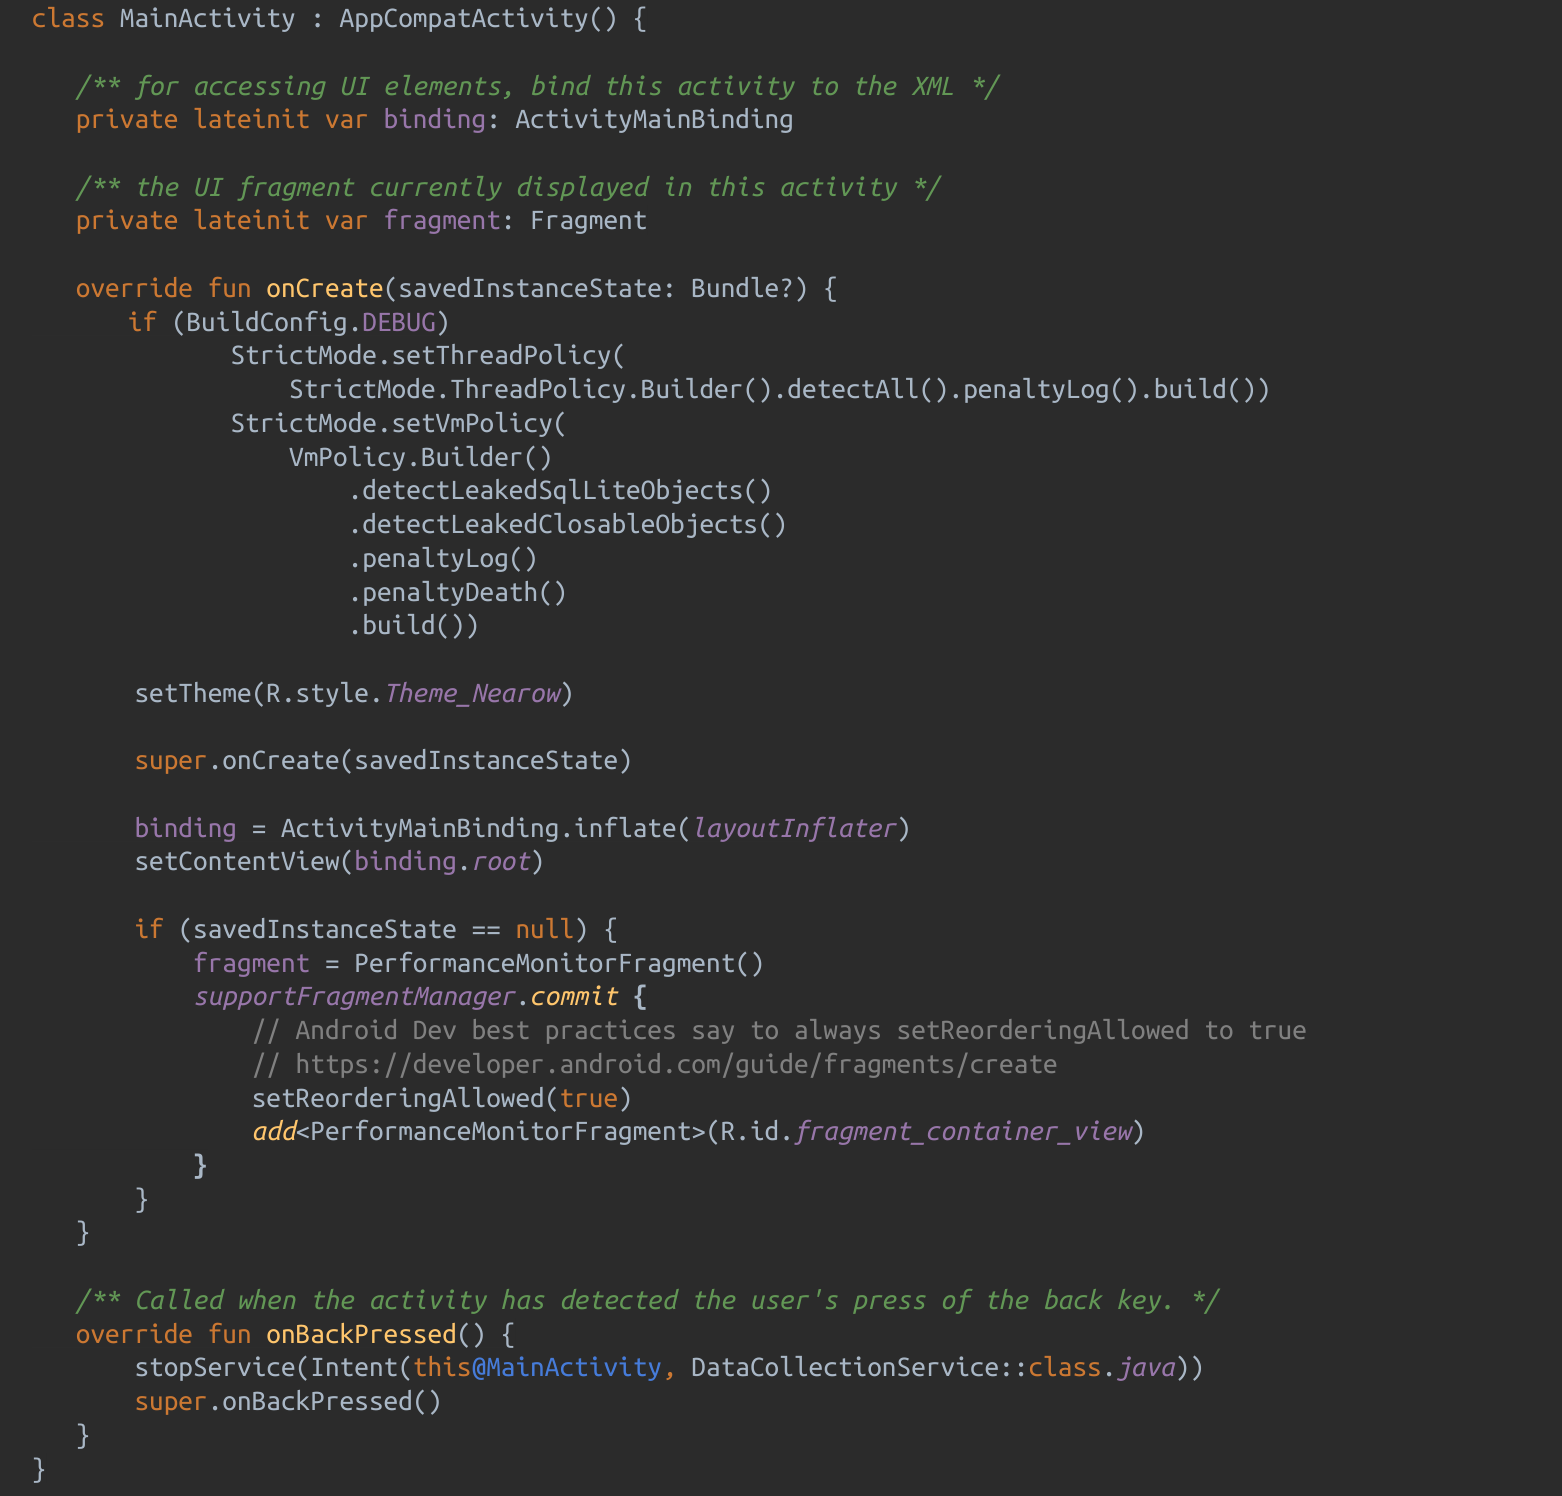
\includegraphics[width=0.9\textwidth]{code-MainActivity.png}
  \caption{}
  \label{fig:MainActivity}
\end{figure}

\texttt{MainActivity.kt} is the entrypoint to the application. It is defined in \texttt{AndroidManifest.xml} as the launcher activity to start the application when its icon is pressed by the user in the app drawer. The class inherits from the \texttt{AppCompatActivity} class, which is the base class (provided by the Google first-party AndroidX library) for activities that wish to use some of the newer platform and design features on older Android devices.

The \texttt{onCreate} method is called when the application is started. If the application is in debug mode, \texttt{StrictMode} is enabled. \texttt{StrictMode} is a developer tool that is used to catch common programming errors and exceptions; it logs any long-running operations that are not explicitly marked as being allowed to run on the main thread, and is used to help determine any causes that are preventing the application from running as smoothly as possible. \texttt{StrictMode} is also configured to shut down the application if a memory leak is detected.

MainActivity is nothing more than a shell for the user interface. The main UI components are detached from the activity and placed in a fragment. This is done so that the fragment remains independent of any activity-specific changes such as screen rotation. However, since fragments are not notified of these changes at all, handling of, for example, a press on the device's back button is performed by the \texttt{MainActivity}. When the back button is depressed, the activity shuts down the \texttt{DataCollectionService} before letting the activity be destroyed.

The fragment displayed in \texttt{MainActivity} is the \texttt{PerformanceMonitorFragment}. It is added to the layout of the \texttt{MainActivity} through the activity's \texttt{supportFragmentManager}.

\subsection{\texttt{PerformanceMonitorFragment.kt}}

This class handles the bulk of the user interface, as described in design section \ref{sec:pmfrag}. The fragment's \texttt{onCreateView} method is automatically called when the fragment is added into an activity; in the context of this application it is only ever added to \texttt{MainActivity}, but in theory this could be any activity.

If the GPS location permission has not been granted when the \texttt{startAndBindToDataCollectionService} subroutine is called, a permissions request is launched (the callback for which is initialised on class instantiation). If the user grants the permission, the service startup method is called again, otherwise a permission information dialog is shown to explain why, with the GPS location permission denied, it will not be possible to let the client make full use of the application. Once GPS location permission has been granted, the service is started. The function call for this is different depending on the Android OS version, as Android Oreo introduced new battery-optimisation features for long-running services. Finally, a bind request is issued so that the fragment can interact with the newly launched instance of the \texttt{DataCollectionService}.

Once (if) binding to the service is successful, the \texttt{onServiceConnected} callback function is launched. This is where the fragment is notified that the service has been bound to. The fragment obtains the \texttt{DataCollectionService} instance from the \texttt{LocalBinder} that is passed to the callback. The fragment then registers itself as the new \texttt{DataUpdateListener} for the service. A private boolean called \texttt{mBound} stores the value of whether there is an established connection with the service, and is set to \texttt{true} when the connection is established. It is appropriately set to \texttt{false} when the \texttt{onServiceDisconnected} callback is activated. This boolean is used in other parts of the class to ensure that a connection to the service still exists prior to making calls that interact with the bound service.

Android view-binding is enabled in the \texttt{build.gradle} buildscript of the project, which means that access to UI components is handled via the automatically generated \texttt{FragmentPerformanceTrackerBinding} class. This means that formerly abundant references to the \texttt{findViewById} function are no longer necessary.

The application toolbar is initialised with two menu elements: the "view sessions" button and a switch to enable or disable GPS. The button for session history is configured with a simple callback to launch the \texttt{SessionsActivity} when pressed. The GPS switch is configured with a function to call, if bound to the service, the \texttt{enableGps} and \texttt{disableGps} methods provided by it. In addition, the UI elements for split and distance are hidden or shown as appropriate depending on whether GPS is enabled.

A \textit{floating action button} (FAB) in the bottom-right corner controls the recording state of the application. When it is pressed, the \texttt{startTracking} method is called, which performs the following tasks:
\begin{itemize}
  \item resets the stopwatch to start counting up from zero,
  \item sets the button to be red with a stop icon,
  \item marks the toolbar actions as \textit{disabled} to prevent accidental touches during a session
  \item calls the \texttt{startRecording} method of the \texttt{DataProcessor} so that stroke rate and location measurements are stored into the database
\end{itemize}
The \texttt{stopTracking} subroutine performs the inverse of the aforementioned tasks; however, it can only be triggered when the FAB is long-pressed by the user.

The code for the \texttt{PerformanceMonitorFragment} starts on the next page.

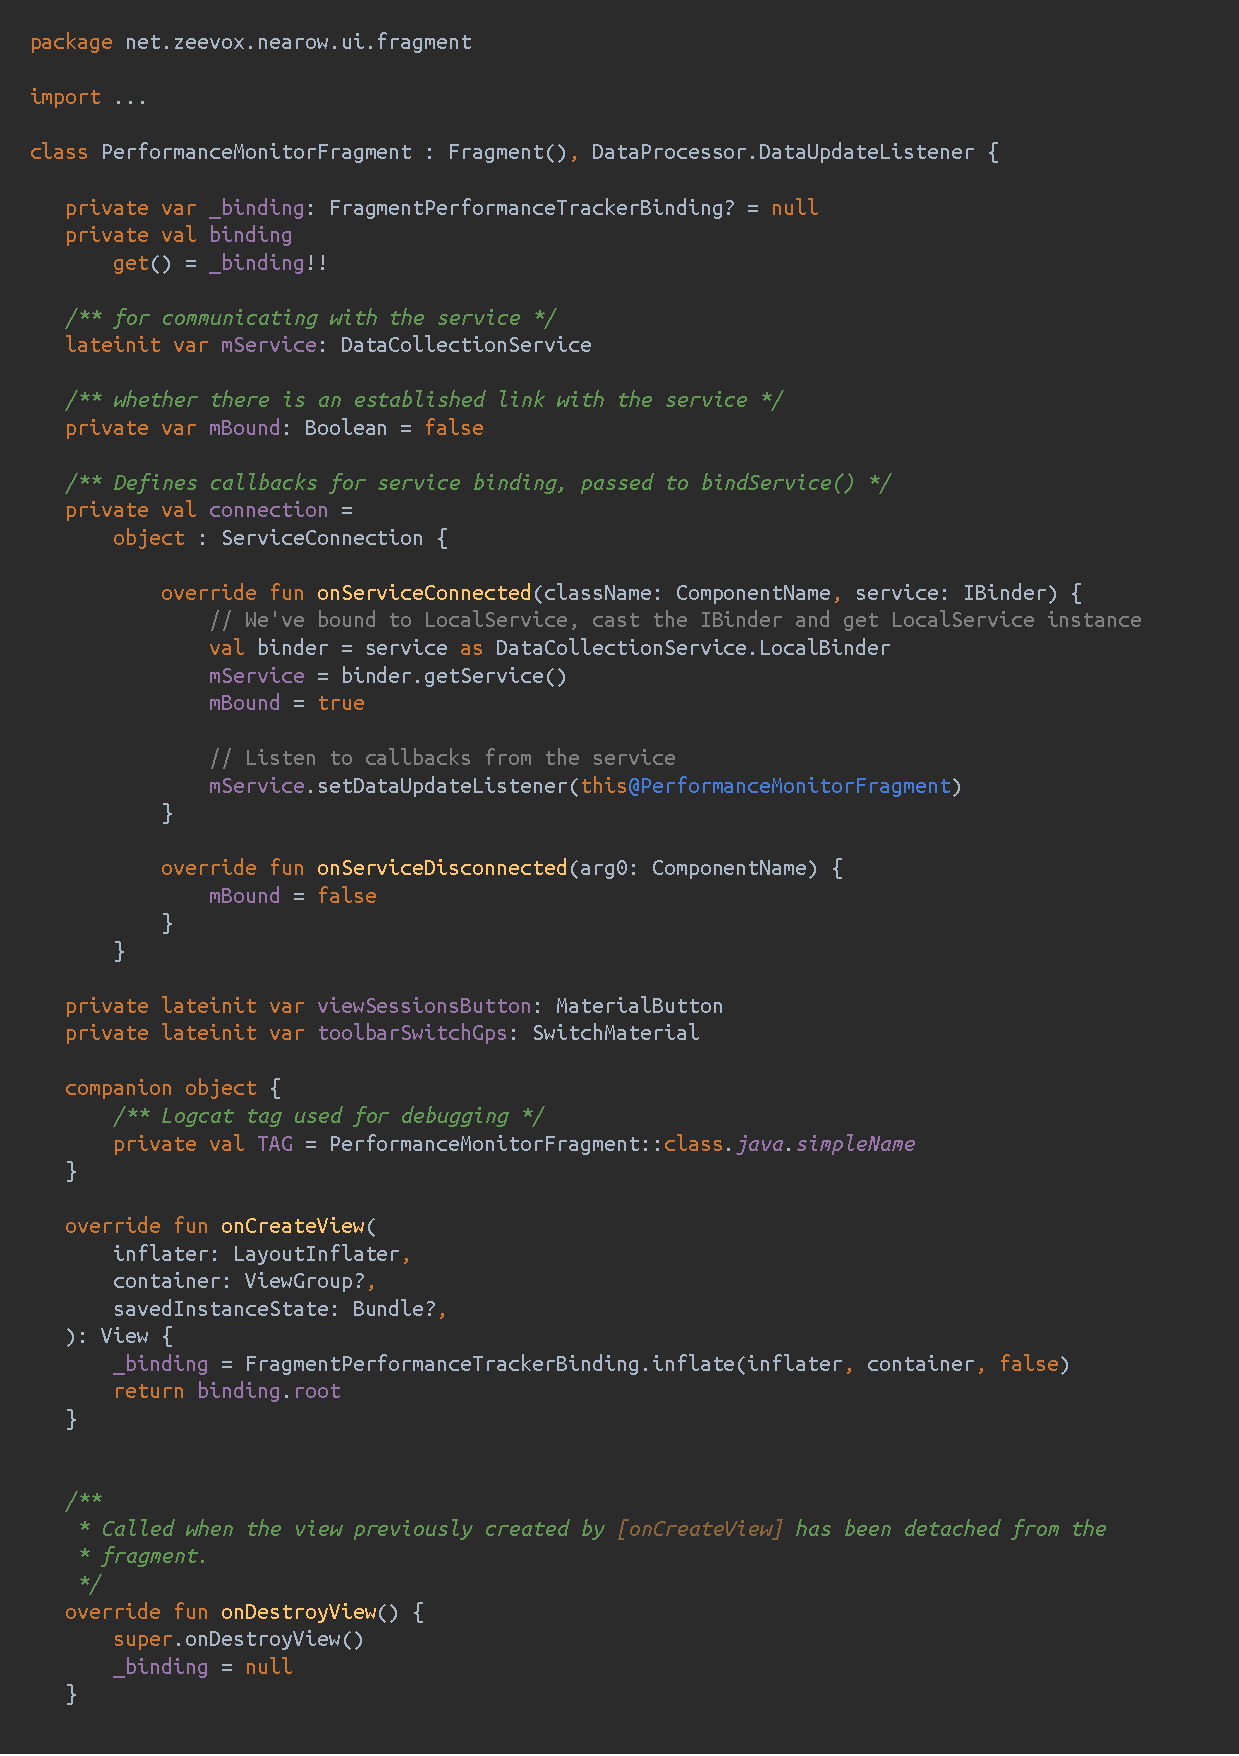
\includepdf[pages=-,pagecommand={},width=1.0\textwidth]{code/PerformanceMonitorFragment.pdf}

\subsection{Recorded sessions view}

In somewhat similar fashion to \texttt{MainActivity} and \texttt{PerformanceMonitorFragment}, \texttt{SessionsActivity} (page \pageref{SessionsActivity}) is a container for the \texttt{SessionsFragment}. The fragment is added to the layout of the \texttt{SessionsActivity} through the activity's \texttt{supportFragmentManager}. The key difference is the addition of a toolbar to the activity, which displays a back arrow and a title. The toolbar back button is configured to act identically to a press on the device back button, returning the user to the main screen.

The \texttt{SessionFragment} also inherits from the Android \texttt{Fragment} base class. A connection to the database is initialised and the list layout is inflated. The \texttt{onCreateView} method sets the adapter used by the \texttt{RecyclerView} to a custom \texttt{SessionsListAdapter}. The \texttt{SessionsListAdapter} class (page \pageref{SessionsListAdapter}) is responsible for populating the list with an element for each recorded session in the database; its parent class is the base \texttt{RecyclerView.ListAdapter} class. This custom child adapter is initialised with a single function as an argument that is called when one of the sessions in the list has its share button pressed. When the \texttt{SessionFragment} is created, it launched a coroutine task to load a list of sessions from the database before calling the list adapter's \texttt{submitList} function to populate the list. The initialisation code for the \texttt{SessionFragment} is presented on page \pageref{SessionsFragment}.

\begin{figure}[h!]
  \centering
  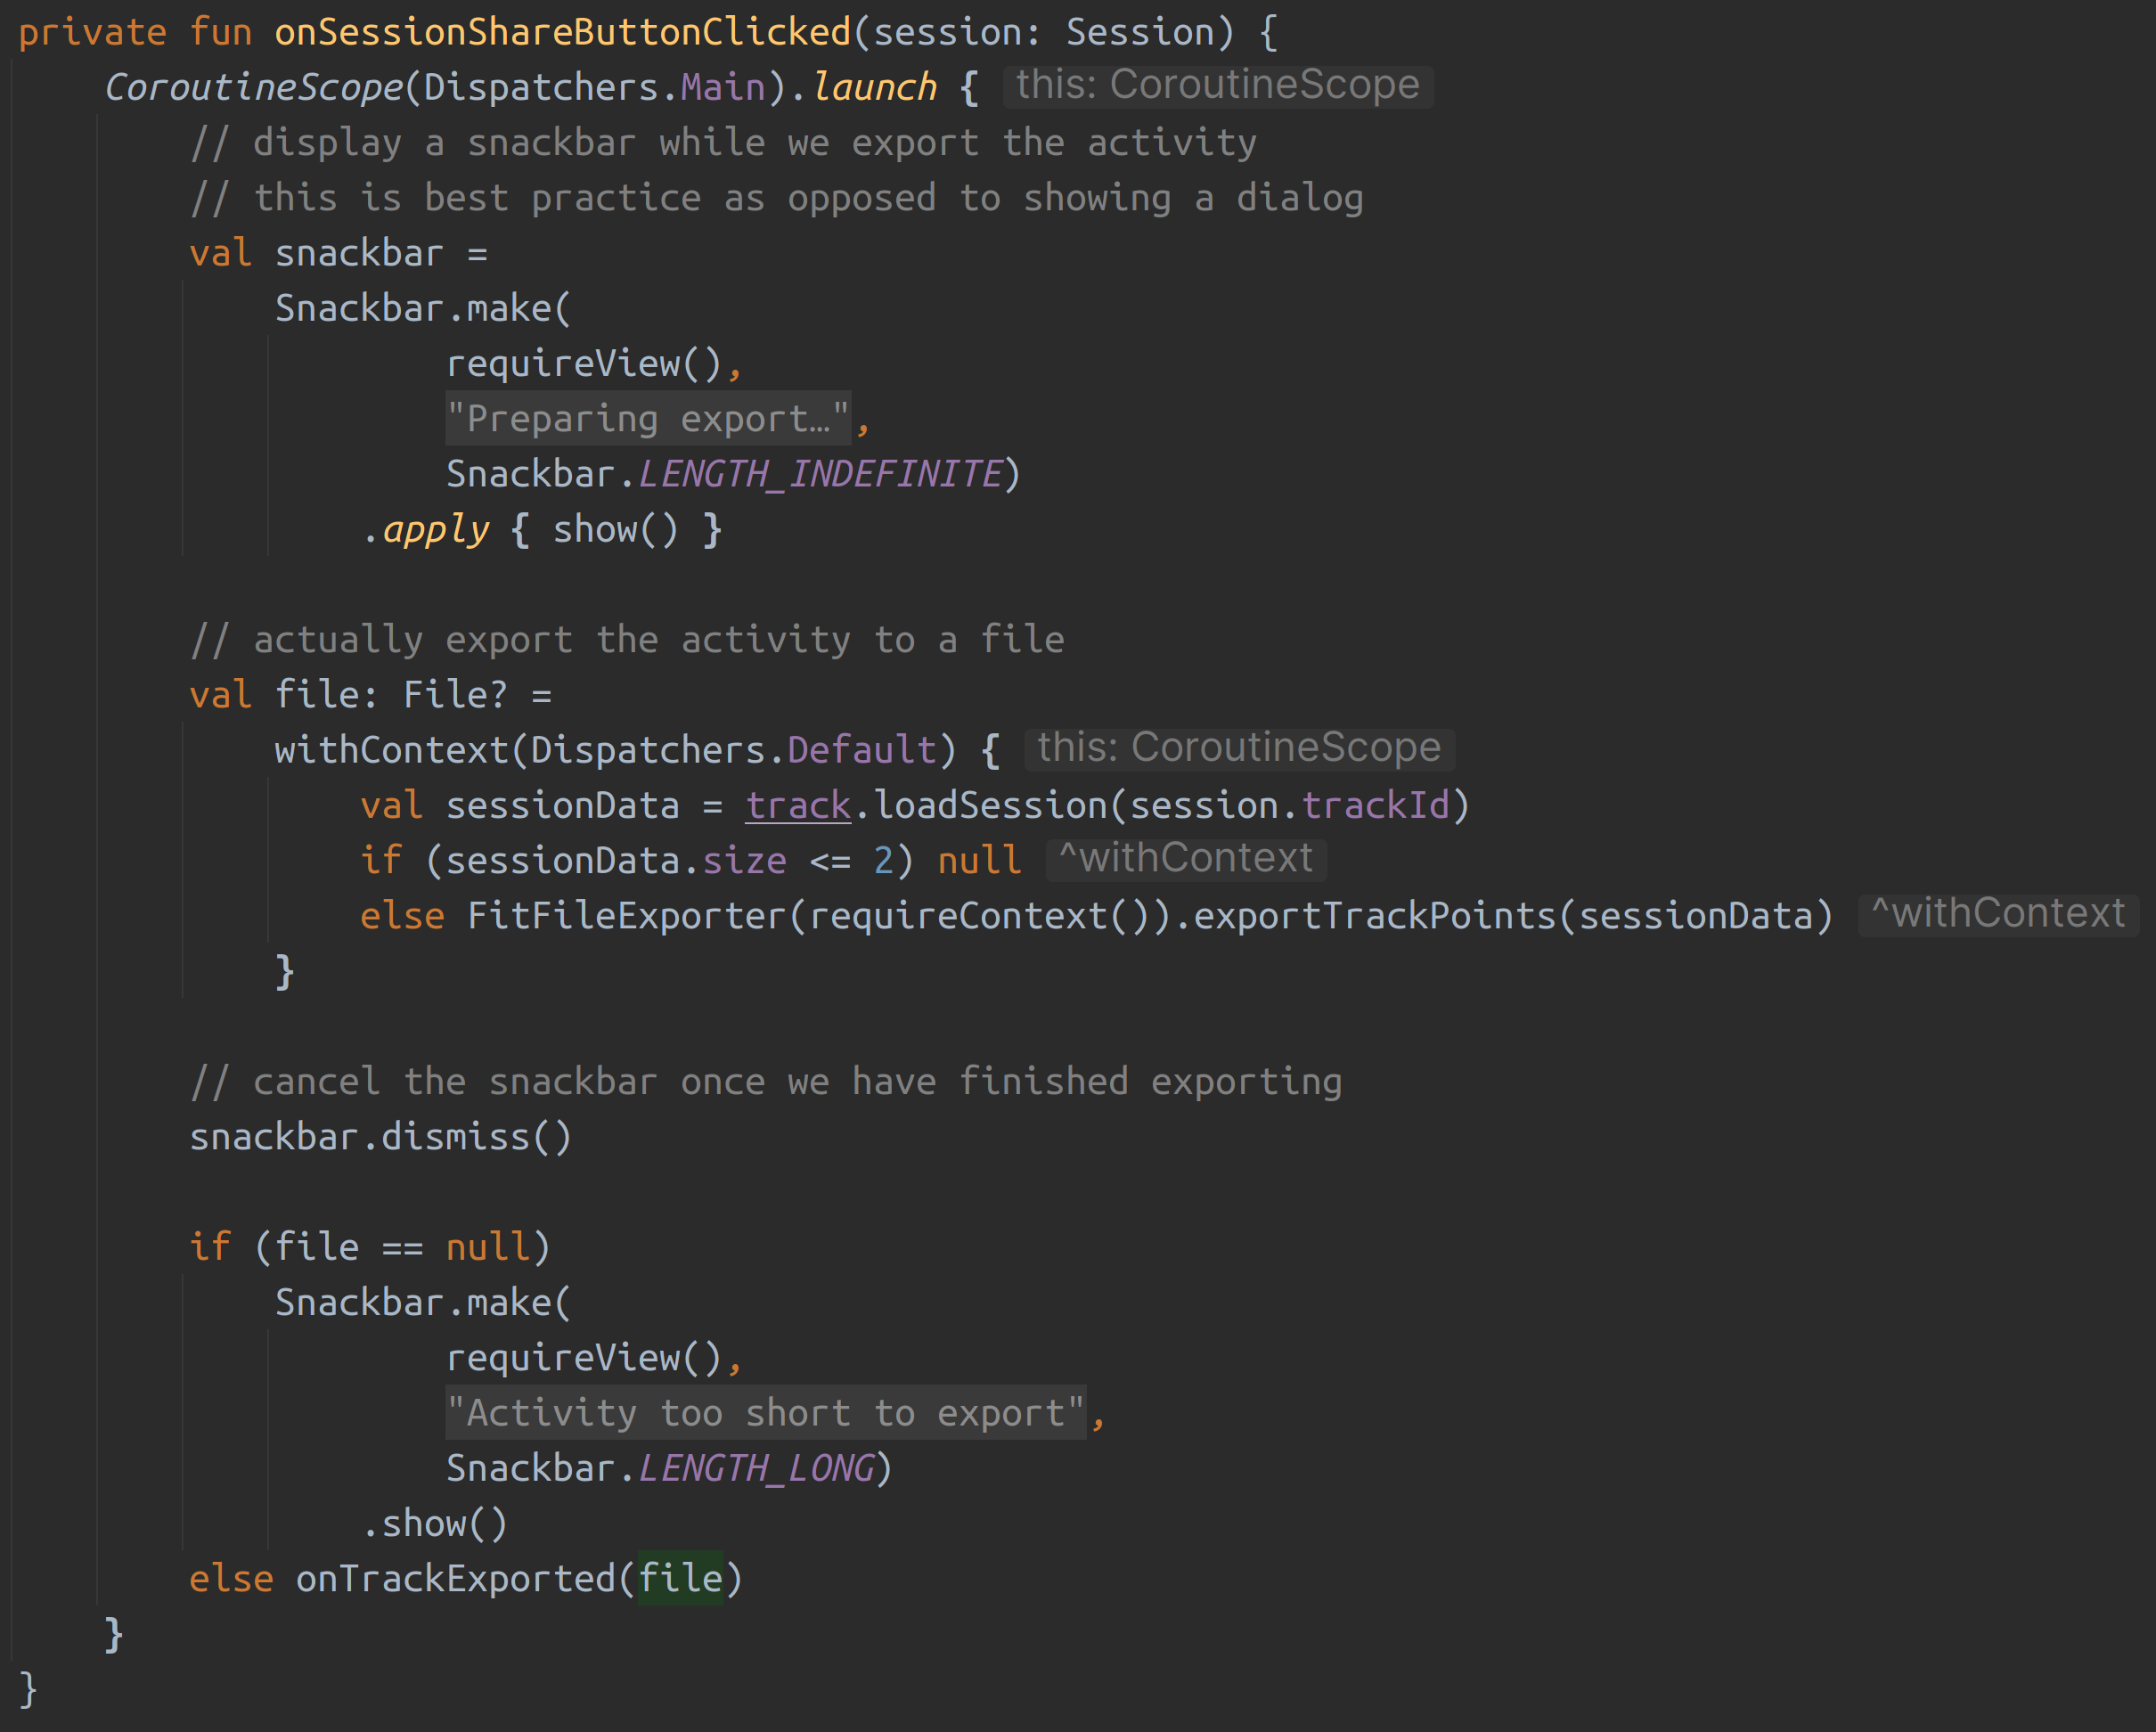
\includegraphics[height=0.4\textheight]{code-onSessionShareButtonClicked.png}
  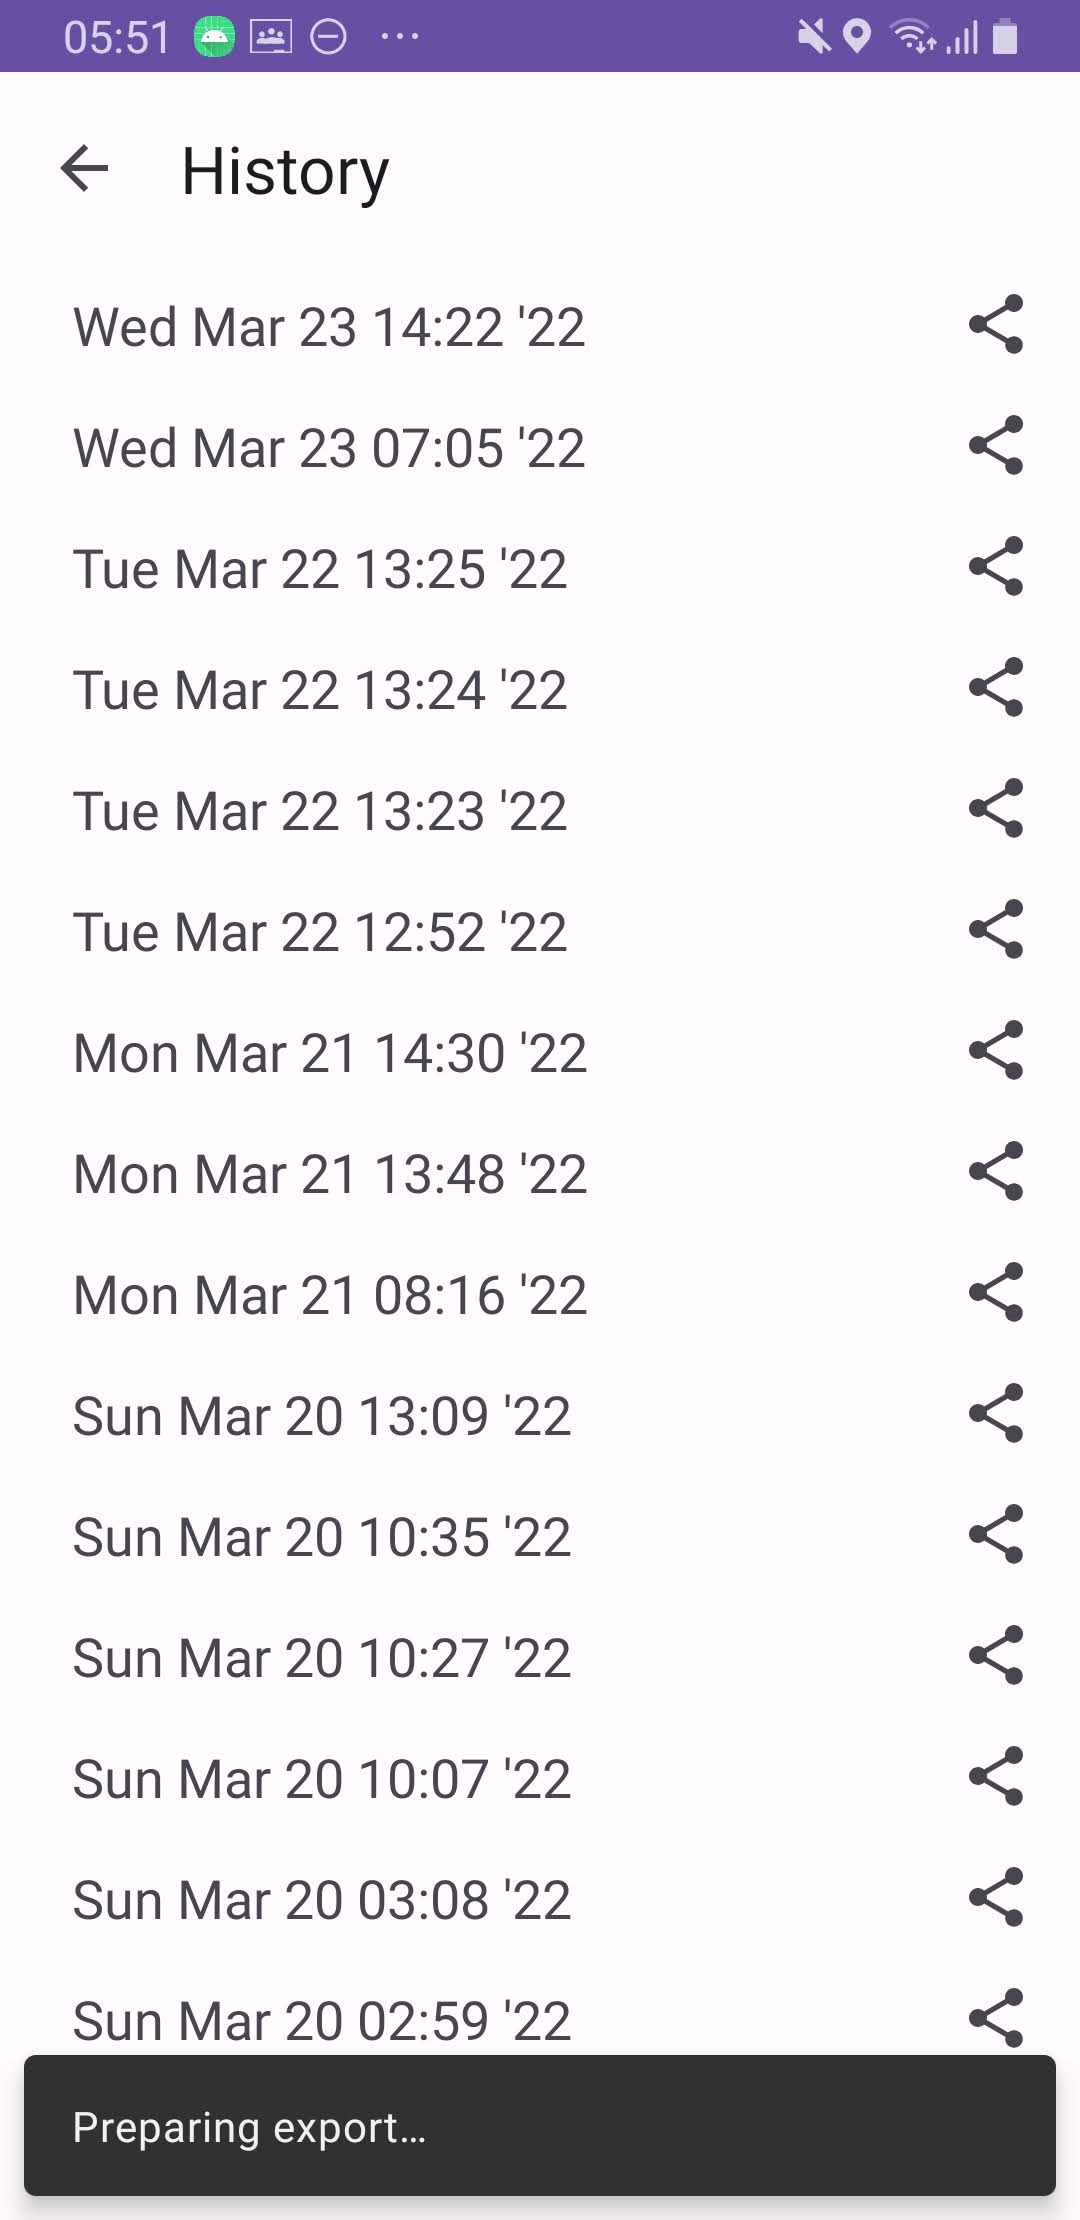
\includegraphics[height=0.4\textheight]{snackbar.jpg}
  \caption{\texttt{onSessionShareButtonClicked} callback function code / snackbar appearance}
  \label{fig:onSessionShareButtonClicked}
\end{figure}

The callback provided to the \texttt{SessionsListAdapter} is the \texttt{onSessionShareButtonClicked} function within the \texttt{SessionsFragment}. The \texttt{onSessionShareButtonClicked} method launches a coroutine task to export the file. While the file is being written, a \textit{snackbar} is shown at the bottom of the screen. A snackbar is the preferred way of doing this, as opposed to a \texttt{progress dialog} which would show a spinny circle in the middle of the screen and block the user from doing anything else. The \texttt{onSessionShareButtonClicked} method is called when the user presses the share button for a session in the list. The \texttt{SessionFragment} loads the points of the recorded session from the database. If there are two or fewer datapoints (incredibly short session) then the export is cancelled. This is because the exporter relies on that fact that there must be a first and last data point for extracting start / stop timestamps. The \texttt{exportTrackPoints} method of the \texttt{FitFileExporter} is called to export the session to a FIT file. If the export is successful, the generated \texttt{File} is passed to the \texttt{onTrackExported} method.

\begin{figure}[h!]
  \centering
  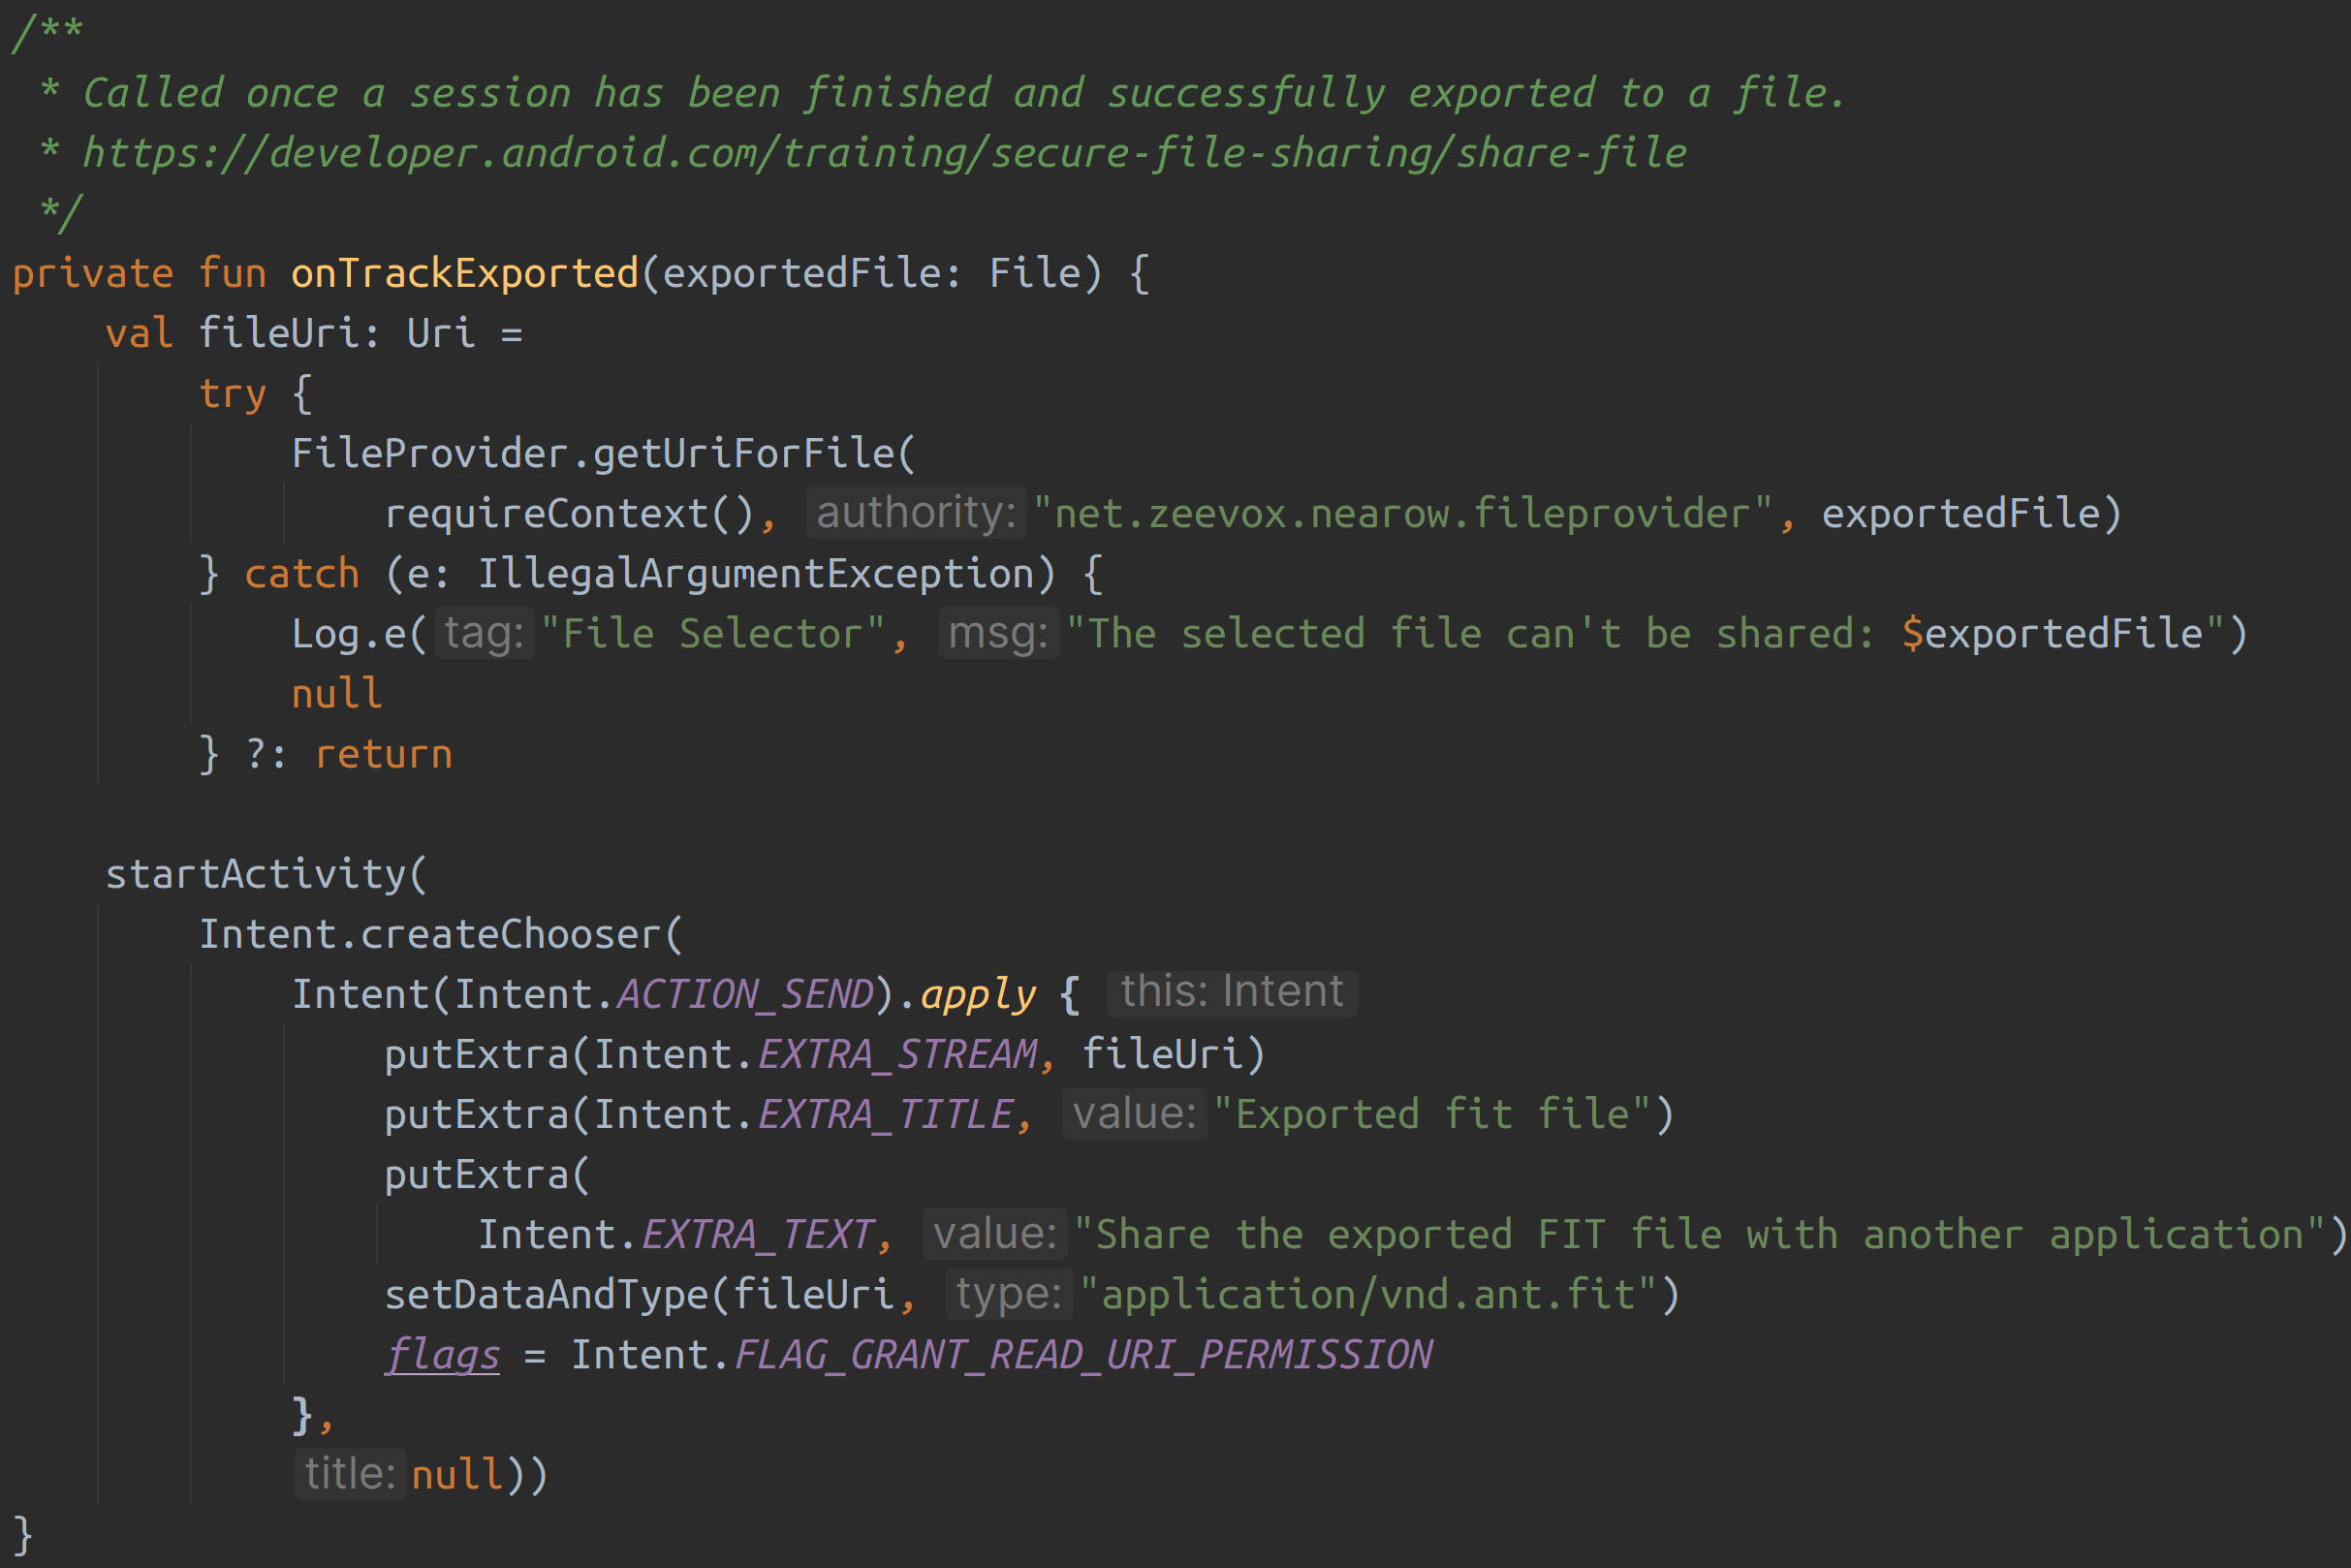
\includegraphics[width=0.9\textwidth]{code-onTrackExported.png}
  \caption{Code for the \texttt{onTrackExported} callback function}
  \label{fig:onTrackExported}
\end{figure}

The \texttt{onTrackExported} method takes in a \texttt{File} and opens an Android \textit{share sheet} that allows the user to send the file to another application installed on the device. Due to the restrictions on file access on Android in the name of privacy concerns, it is necessary to initialise a \texttt{FileProvider} that can then grant temporary read access to the receiving application. The file provider is registered in the \texttt{AndroidManifest.xml} and points to a \texttt{filepaths.xml} file shipped with the application that enumerates specific directories that can be shared from. The exported file is exported into the \texttt{exports/} directory of the internal application storage area. The \texttt{FileProvider} is then used to generate a URI for the exported file. The URI is then passed to the \texttt{Intent} that is used to launch the share sheet. Additional metadata is recorded into the intent, including the file mime type \texttt{application/vnd.ant.fit}\cite{noauthor_flexible_2020}.

\chapter{Testing}

The \href{https://github.com/PhilJay/MPAndroidChart}{\texttt{MPAndroidChart}} library was used to display realtime charts of incoming data for debug purposes.

\begin{figure}[h!]
  \centering
  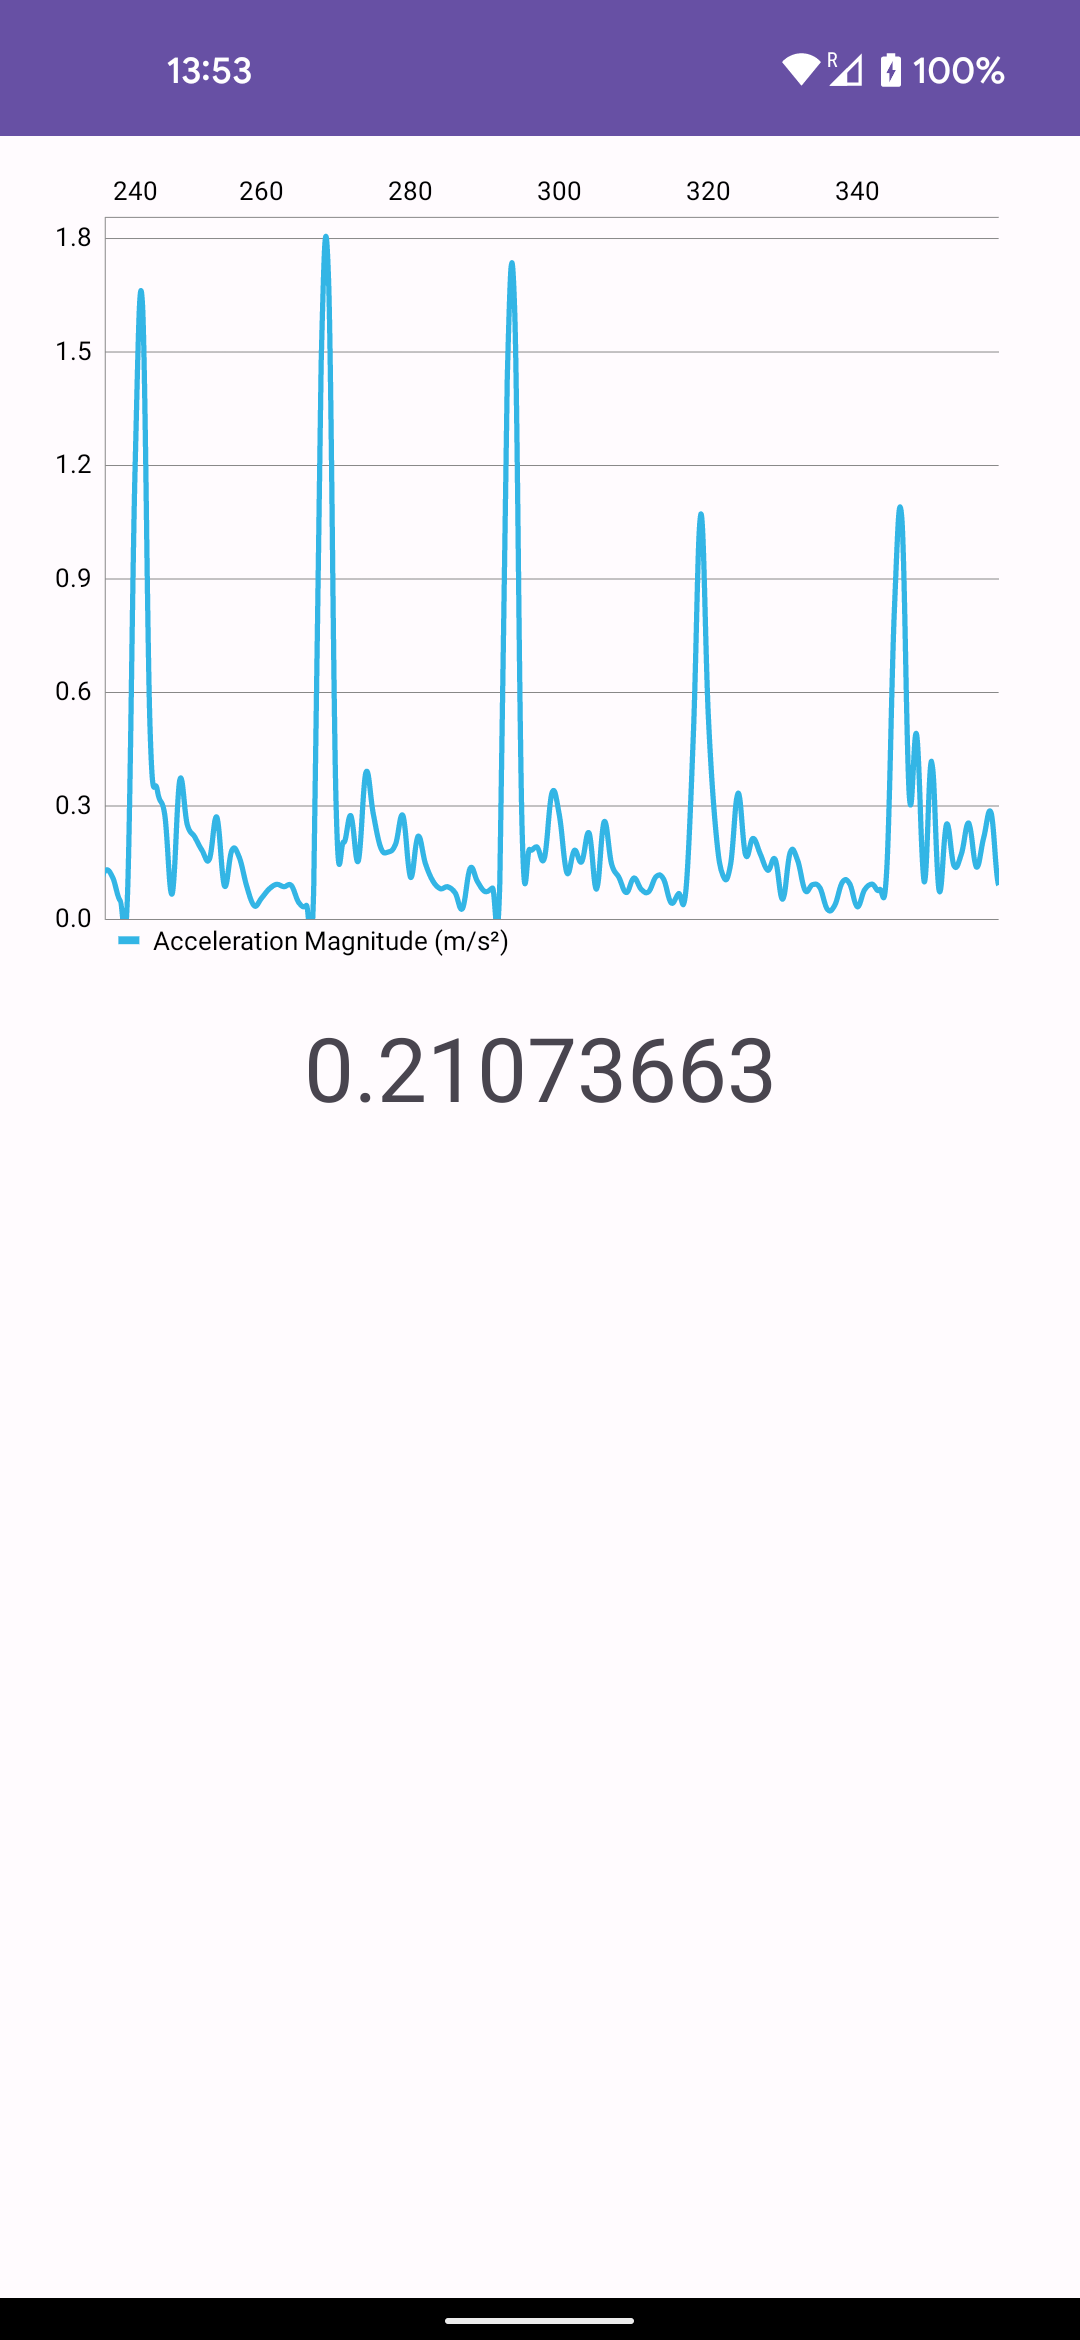
\includegraphics[width=0.3\textwidth]{app-screenshot-accel-graph.png}
  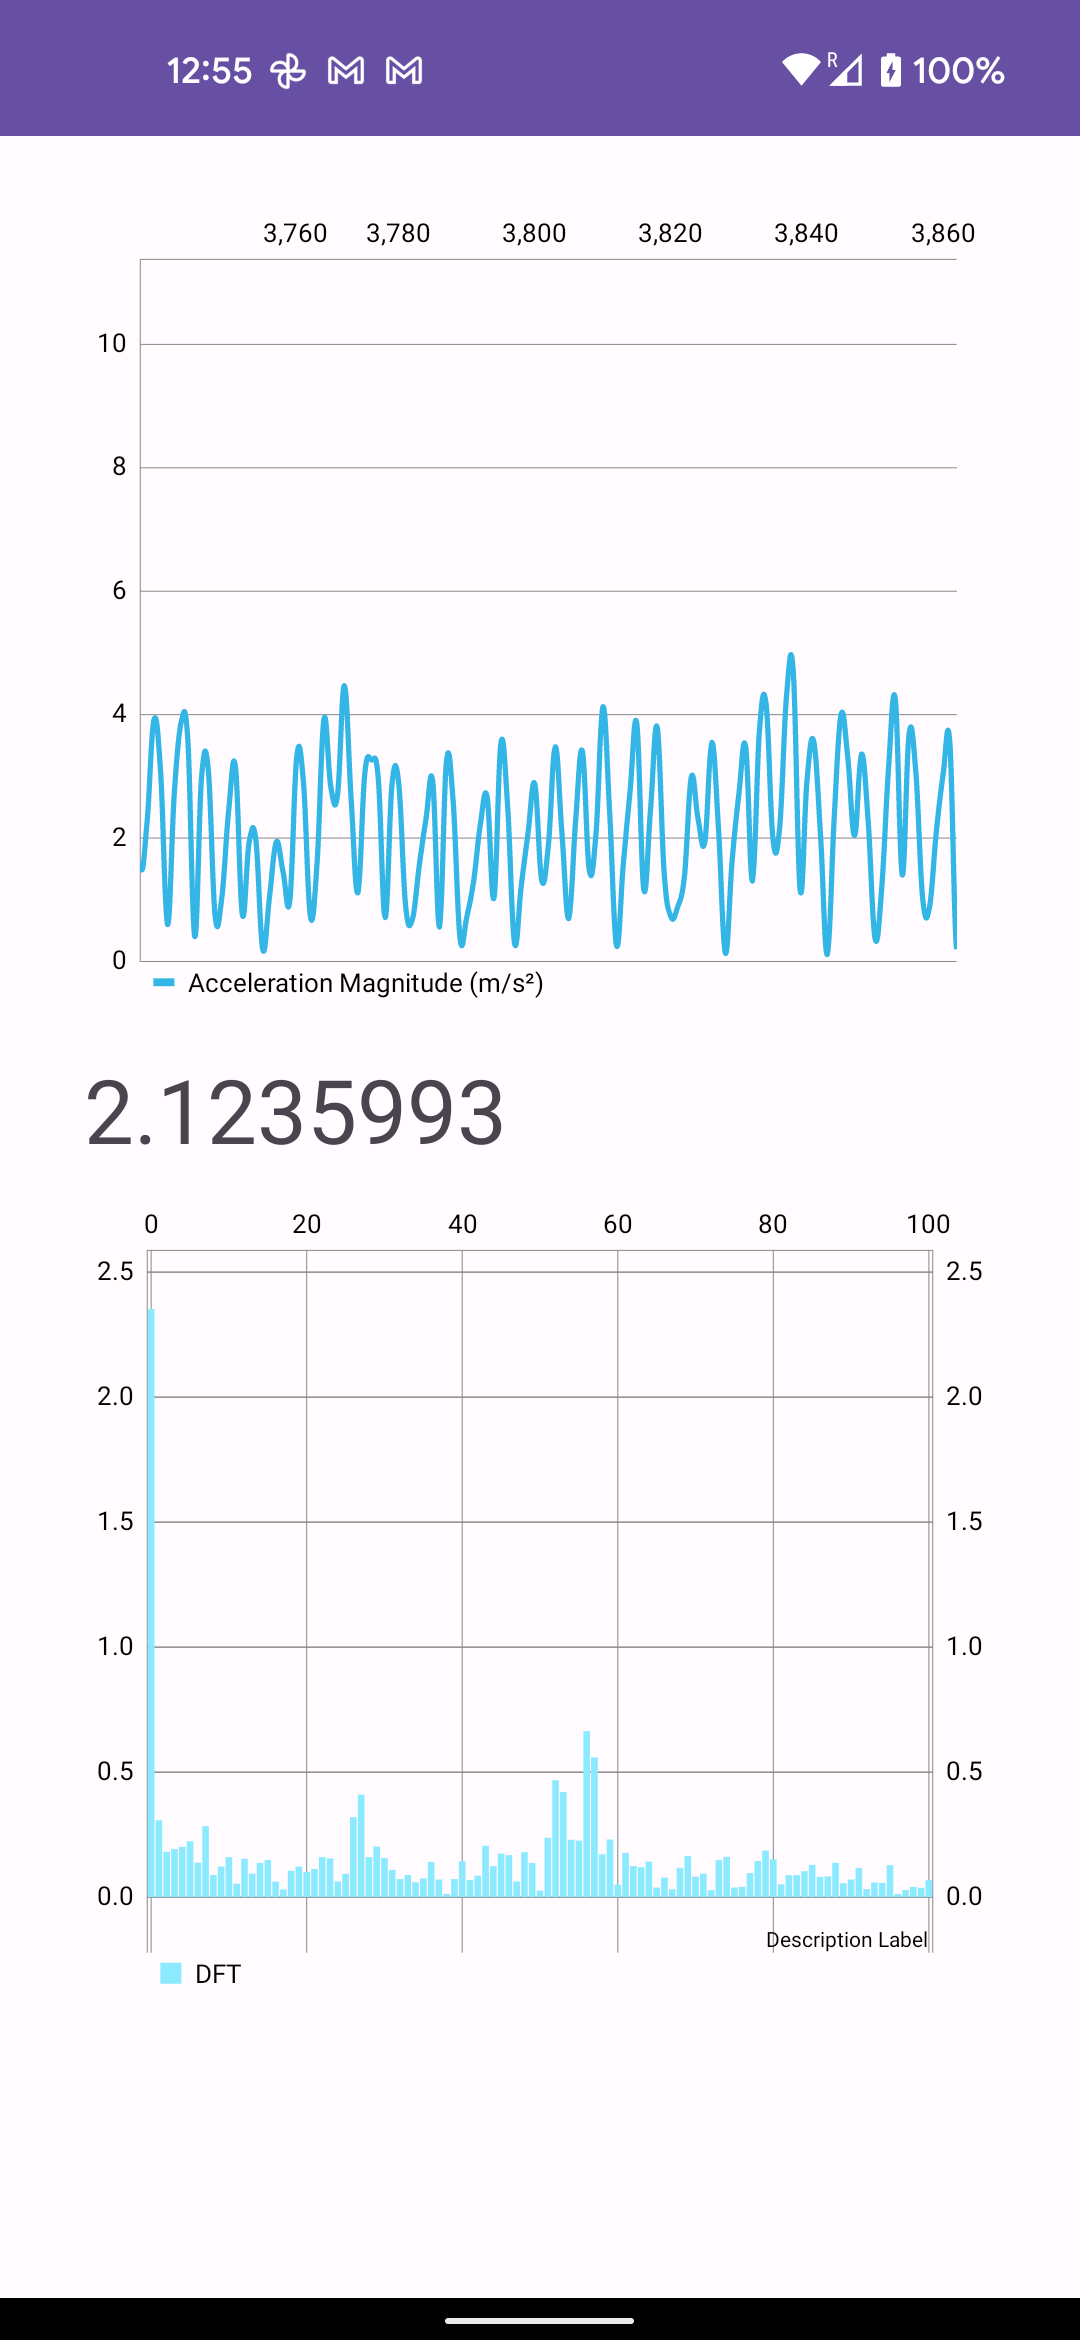
\includegraphics[width=0.3\textwidth]{app-screenshot-accel-with-dft.png}
  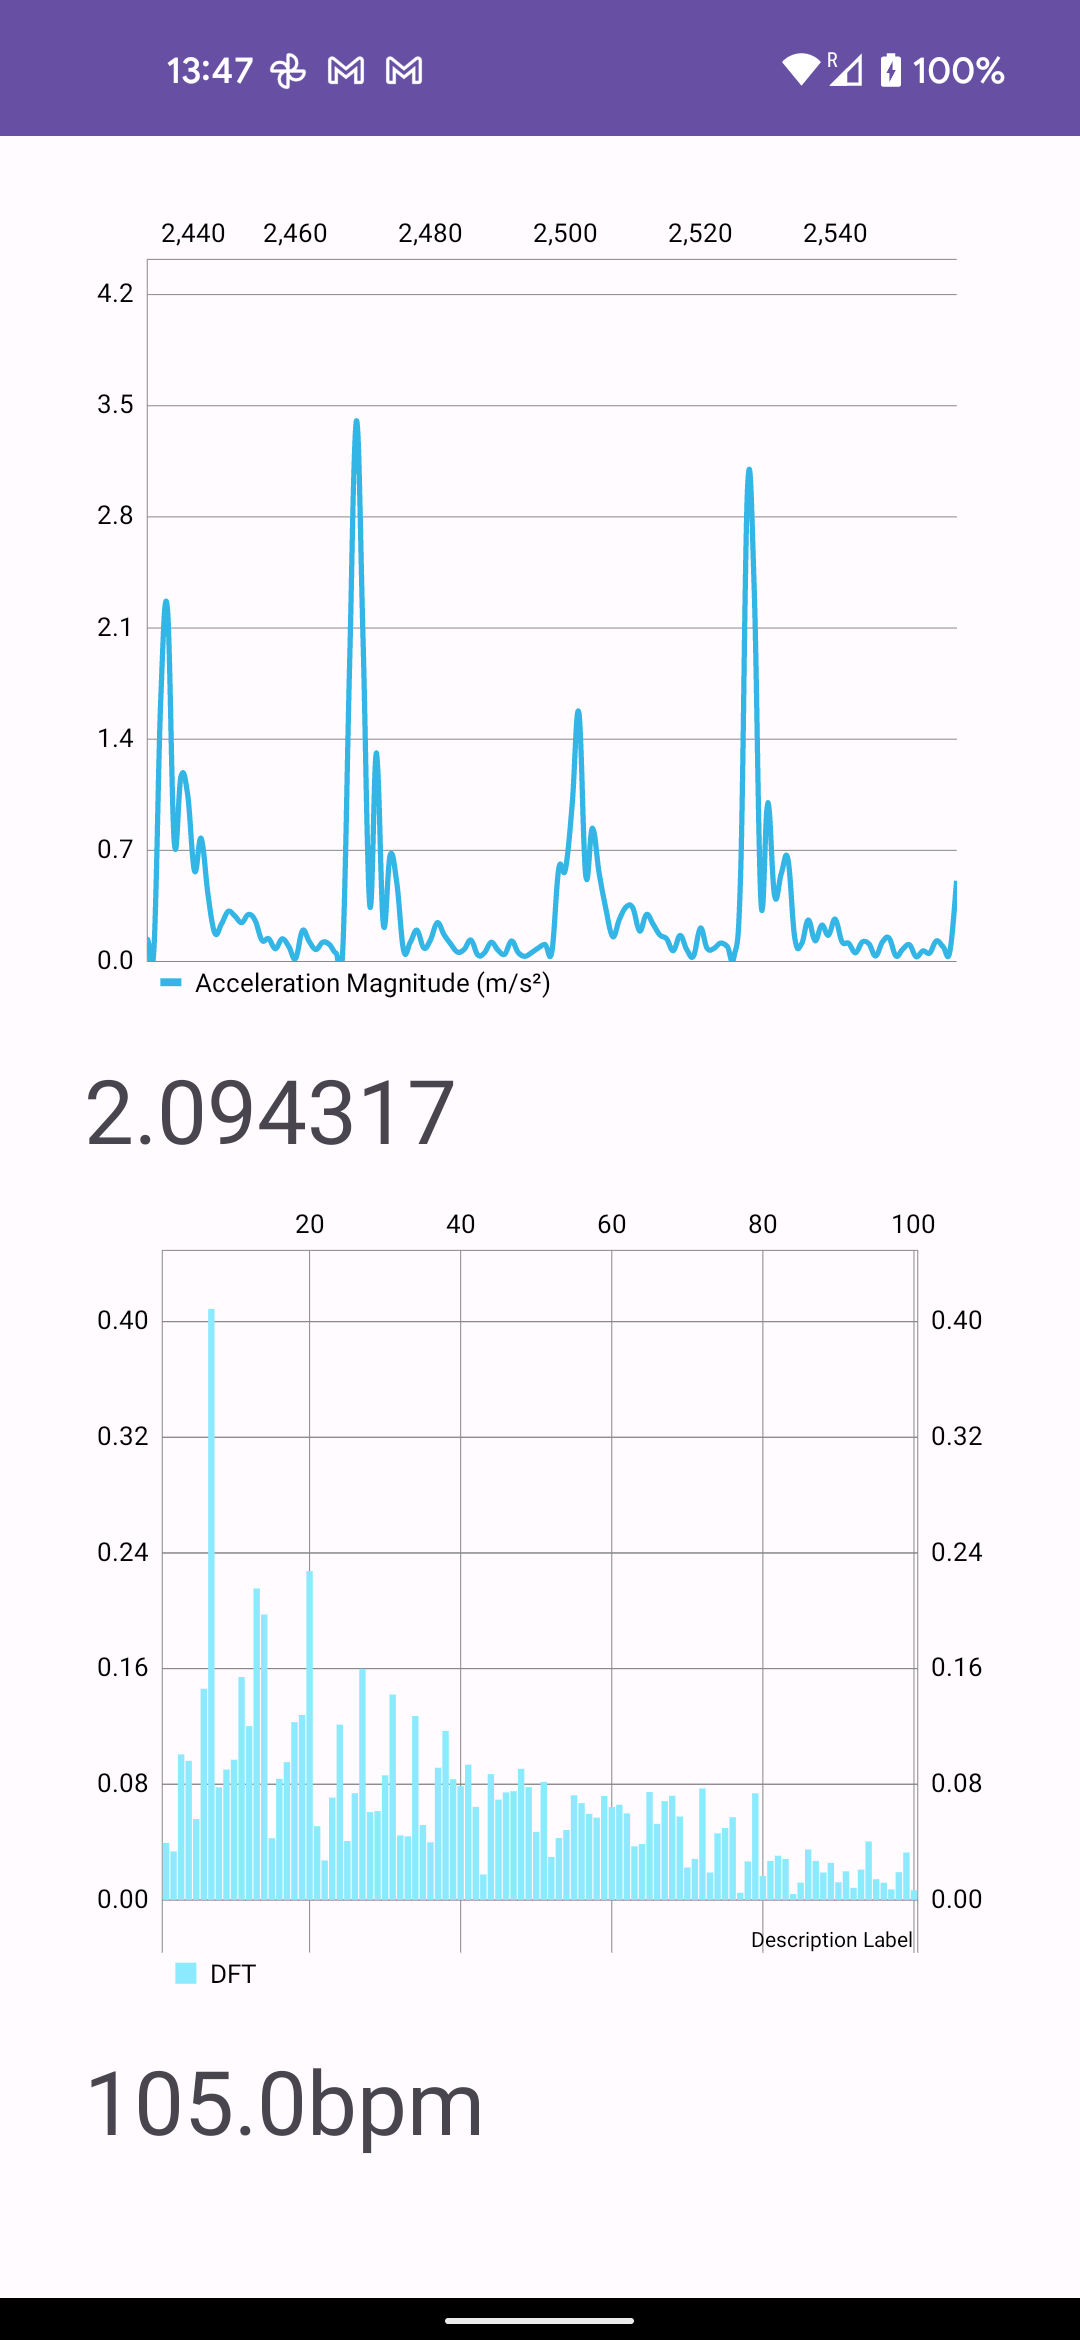
\includegraphics[width=0.3\textwidth]{app-screenshot-accel-with-dft-105-bpm-metronome.png}
  \caption{Iterations of the stroke rate debugger view}
  \label{fig:appscreenshotaccel}
\end{figure}

The first screenshot in figure \ref{fig:appscreenshotaccel} shows the acceleration pattern produced by tapping the phone periodically. A realtime smoothed line chart is updated on every new acceleration reading.

By the time the second screenshot in \ref{fig:appscreenshotaccel} was taken, a bar chart was added to the view to show the amplitude of each frequency bin in the Discrete Fourier transform. The acceleration pattern is that for shaking the phone wildly (small period), which is why the peak in the Fourier transform is nearer to the top of the chart. 

The third screenshot of \ref{fig:appscreenshotaccel} is once again of tapping the phone, but this time to a metronome set to 105bpm. The app correctly detects 105bpm. Admittedly, this specific frequency was not chosen by accident. It is, of course, way more frequent than a rowing stroke could ever be. With a window size of 256 samples, it was empirically determined that stroke rate was accurate to roughly the nearest $\sim6$bpm. In this context, that meant that it would in essence round to one of these stroke rates: $\ldots, 99, 105, 111, \ldots$.

\begin{figure}[h!]
  \centering
  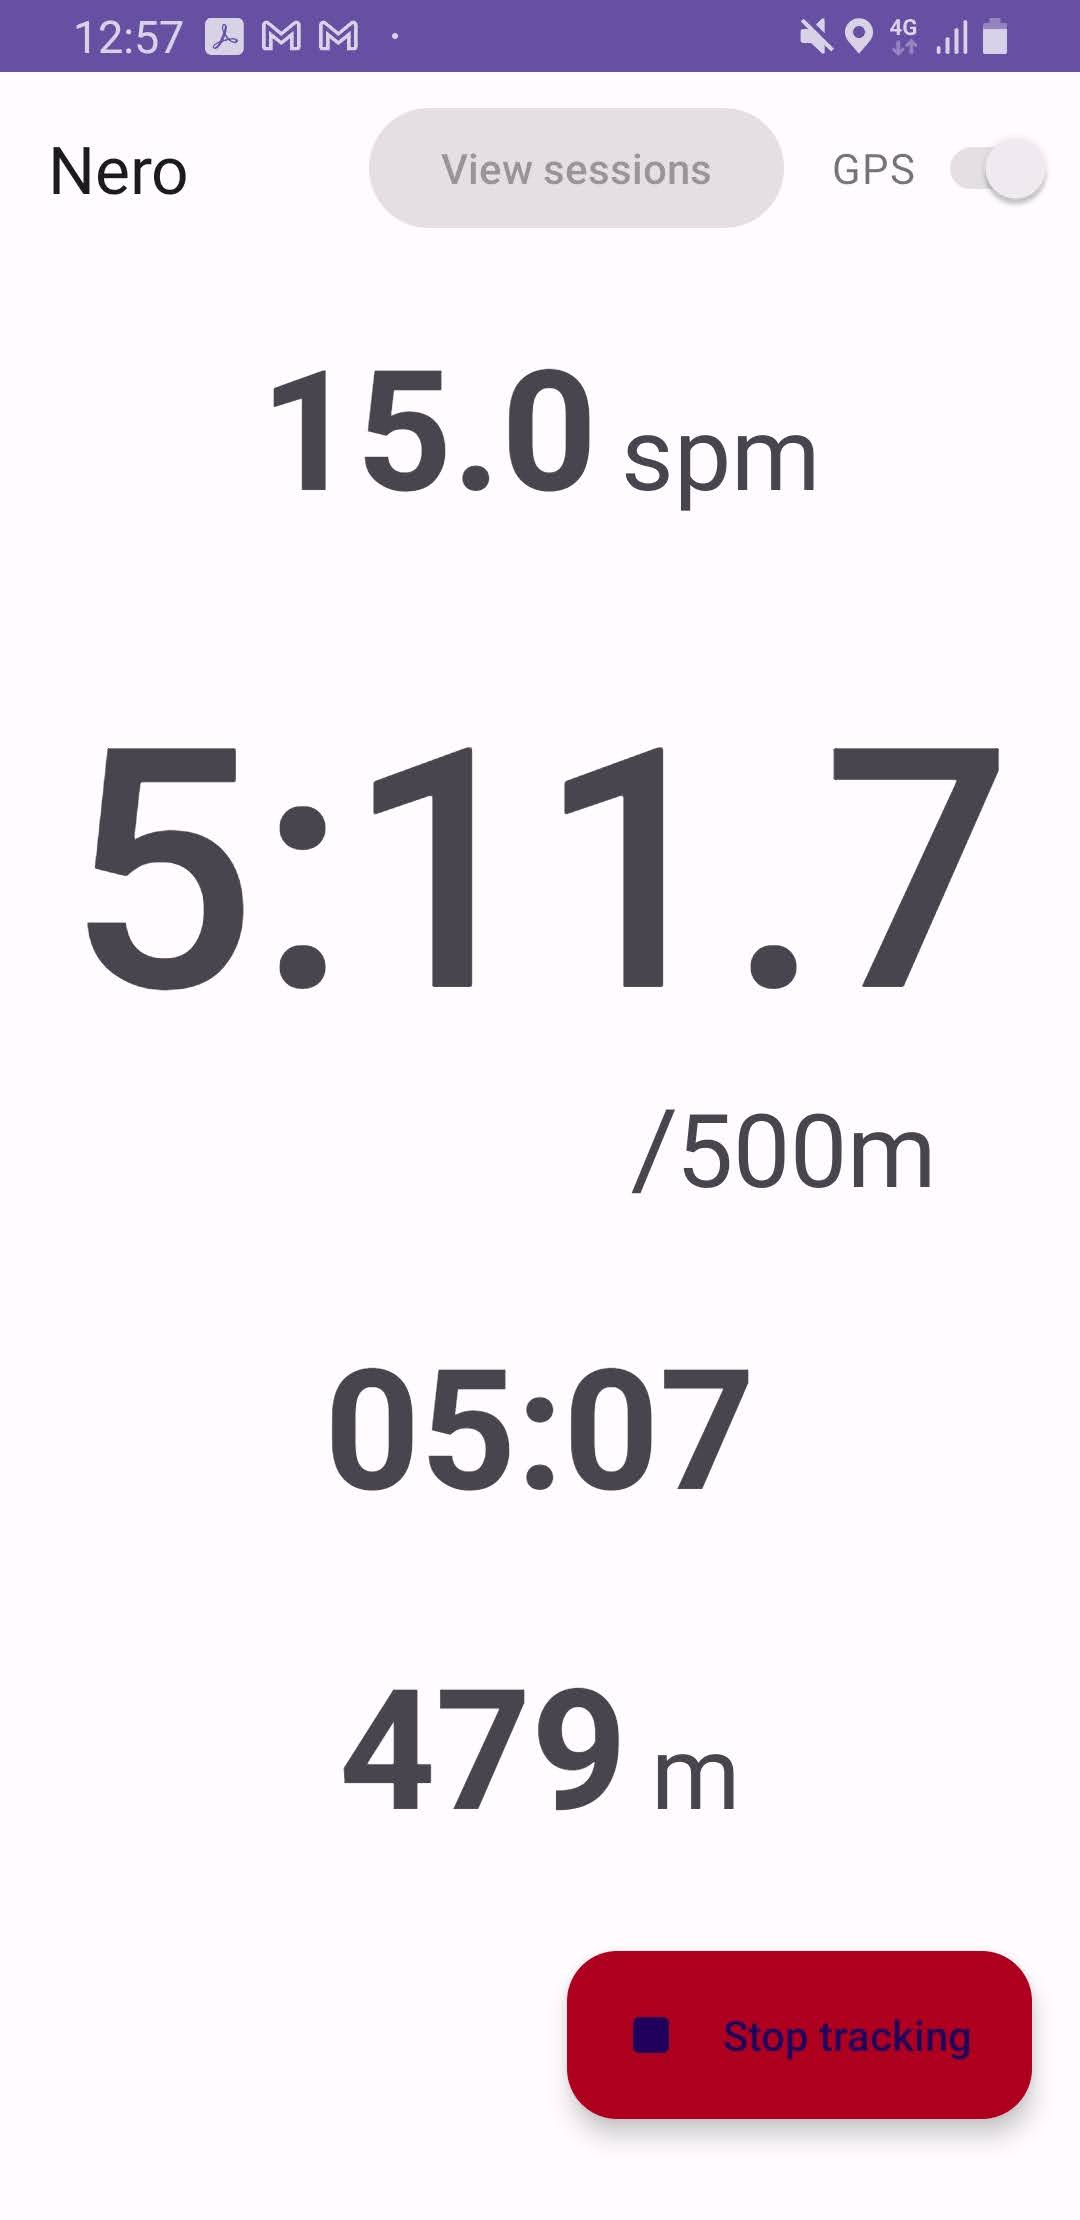
\includegraphics[width=0.3\textwidth]{appworking.jpg}
  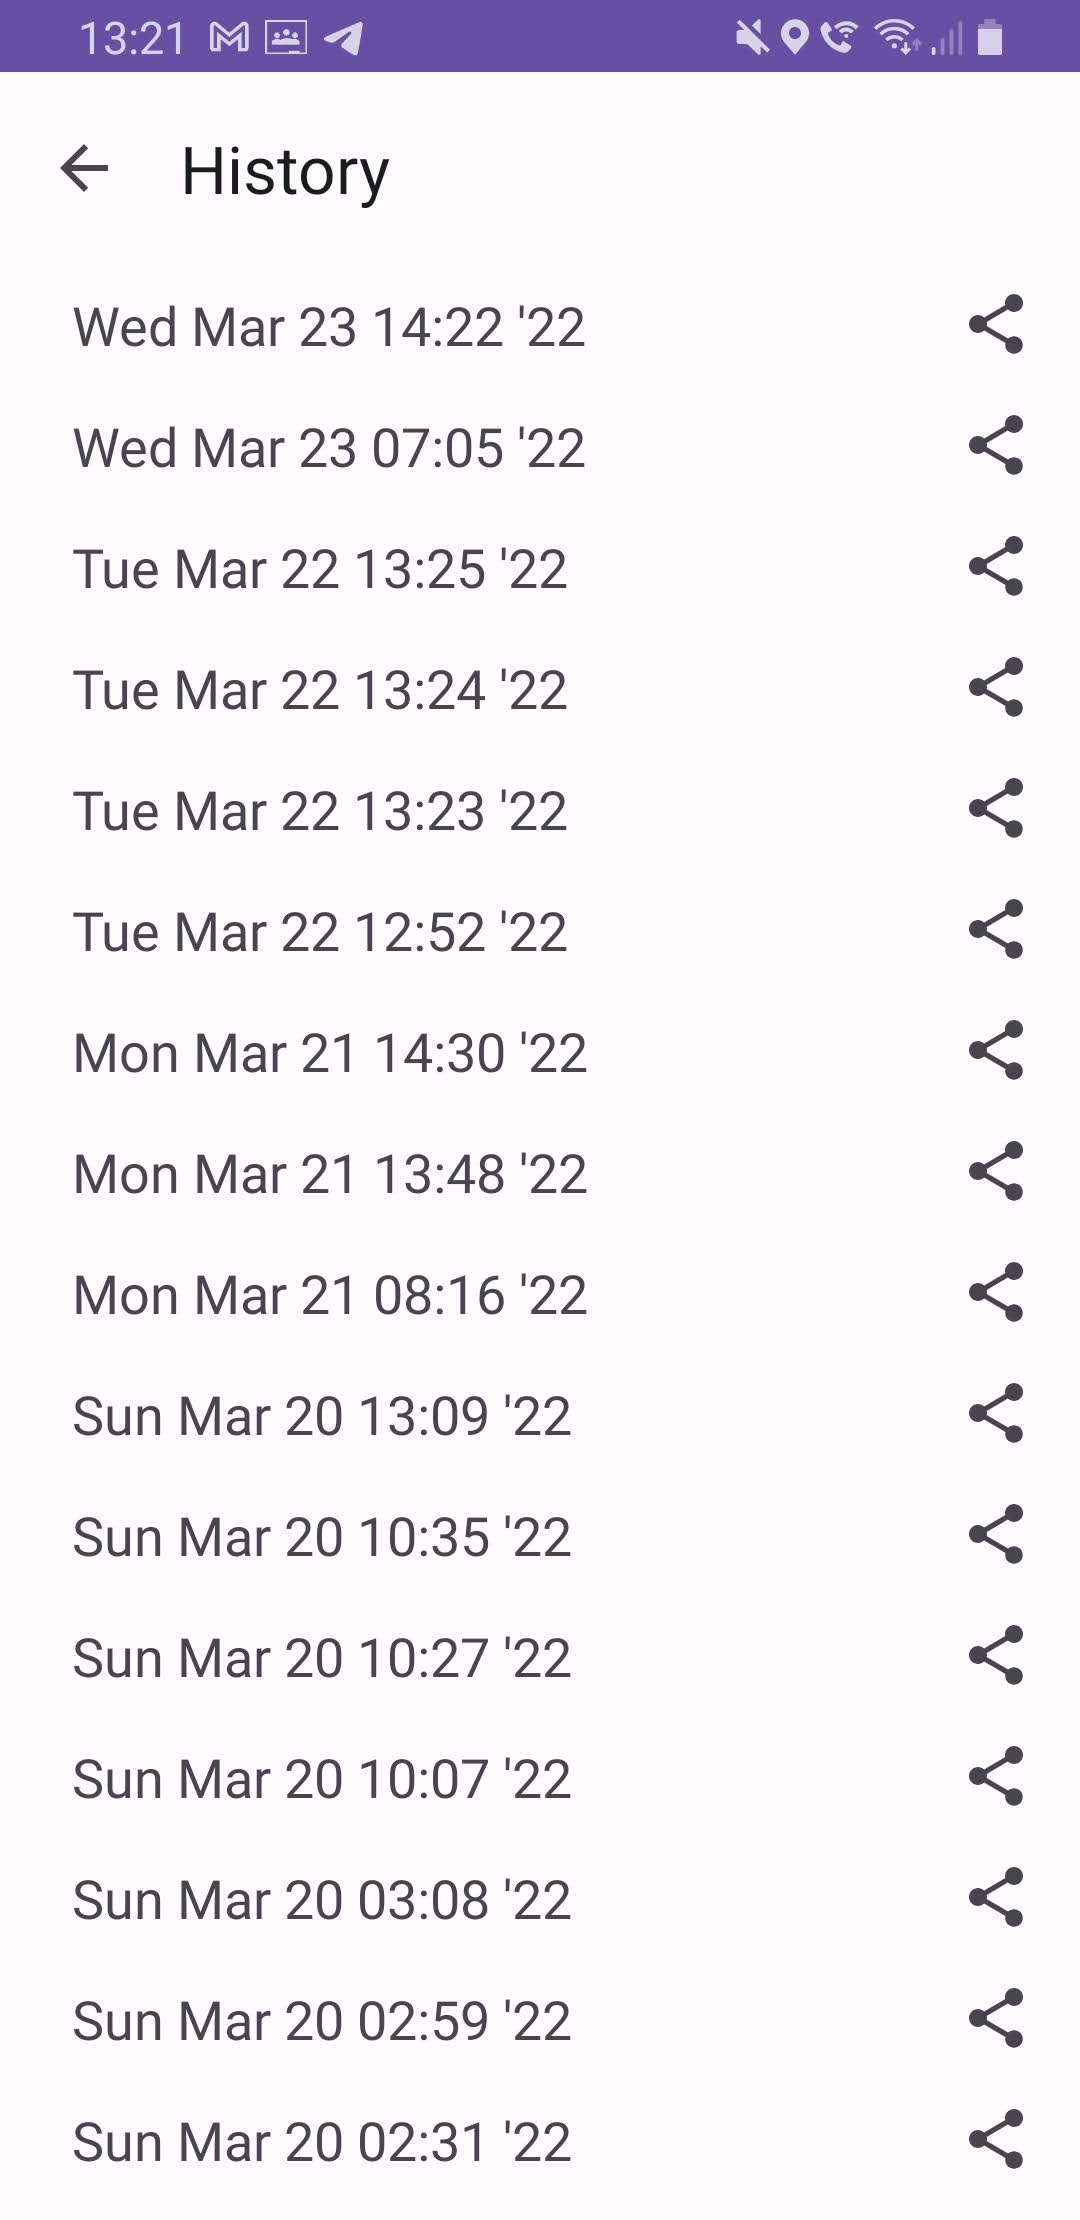
\includegraphics[width=0.3\textwidth]{viewsessions.jpg}
  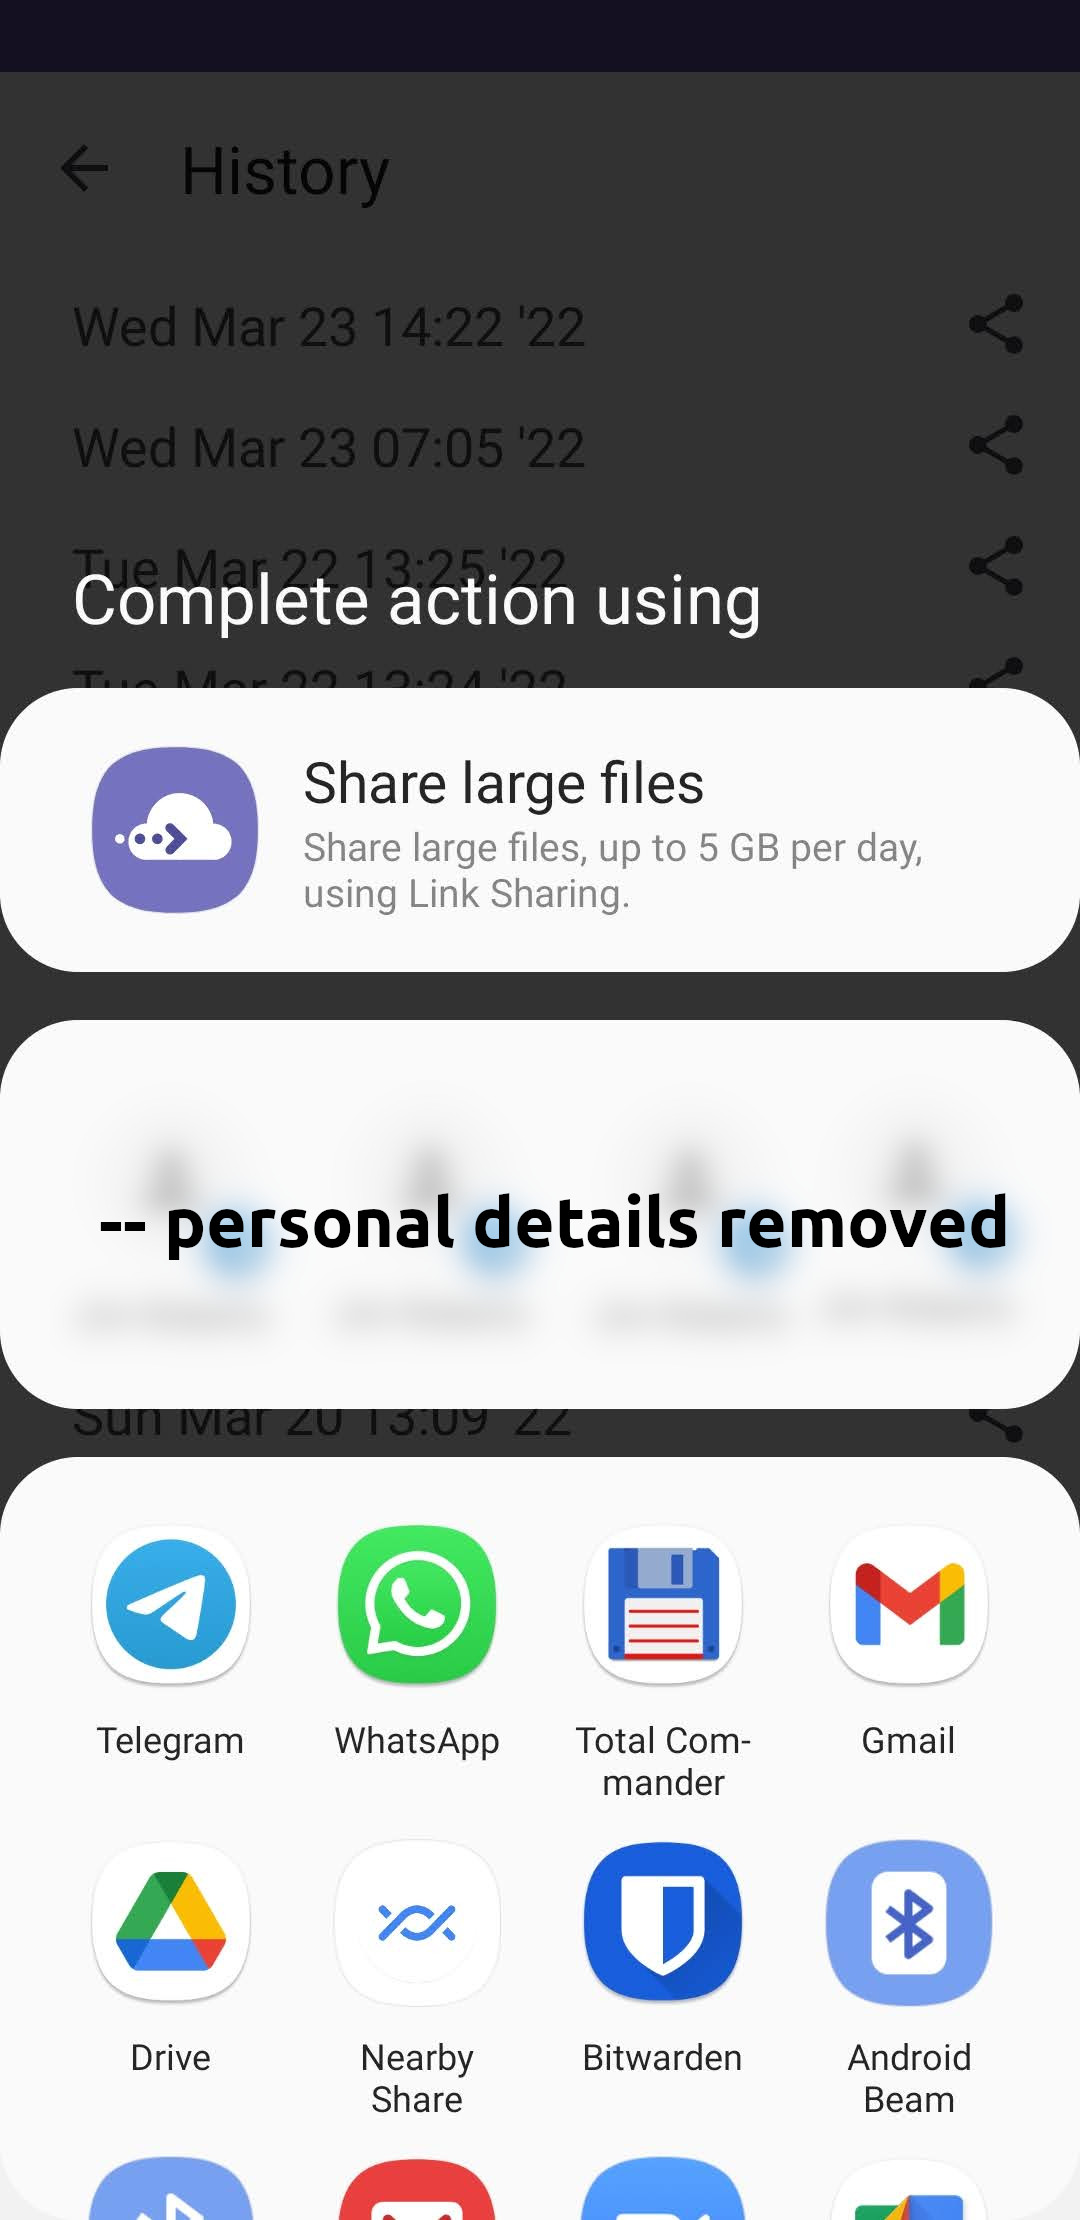
\includegraphics[width=0.3\textwidth]{sharesheet.jpg}
  \caption{application tracking view / session history / session export share sheet}
  \label{fig:appscreenshotworking}
\end{figure}

With the new autocorrelation algorithm in place, the application was tested on the water with a waterproof Samsung Galaxy S8 and Google Pixel 2. Displayed stroke rates seemed plausible, and were usually within a split of the SpeedCoach.

After the outing, the session was exported to the user's devices. The exported FIT file was imported into Strava for further analysis. Average stroke rate matched, the SpeedCoach reported $17.5$ and Strava $18$ (it rounds to the nearest integer). Average split was similar, albeit slightly lower than a SpeedCoach. This is presumed to be because the StrokeCoach does not record the time when the boat drifts with the stream, whereas the application does, increasing the total distance covered. The total distance covered was $6\%$ greater than that reported by the SpeedCoach. This is within acceptable margins of error, but suggests that stillness detection can still be worked on.

\begin{figure}[h!]
  \centering
  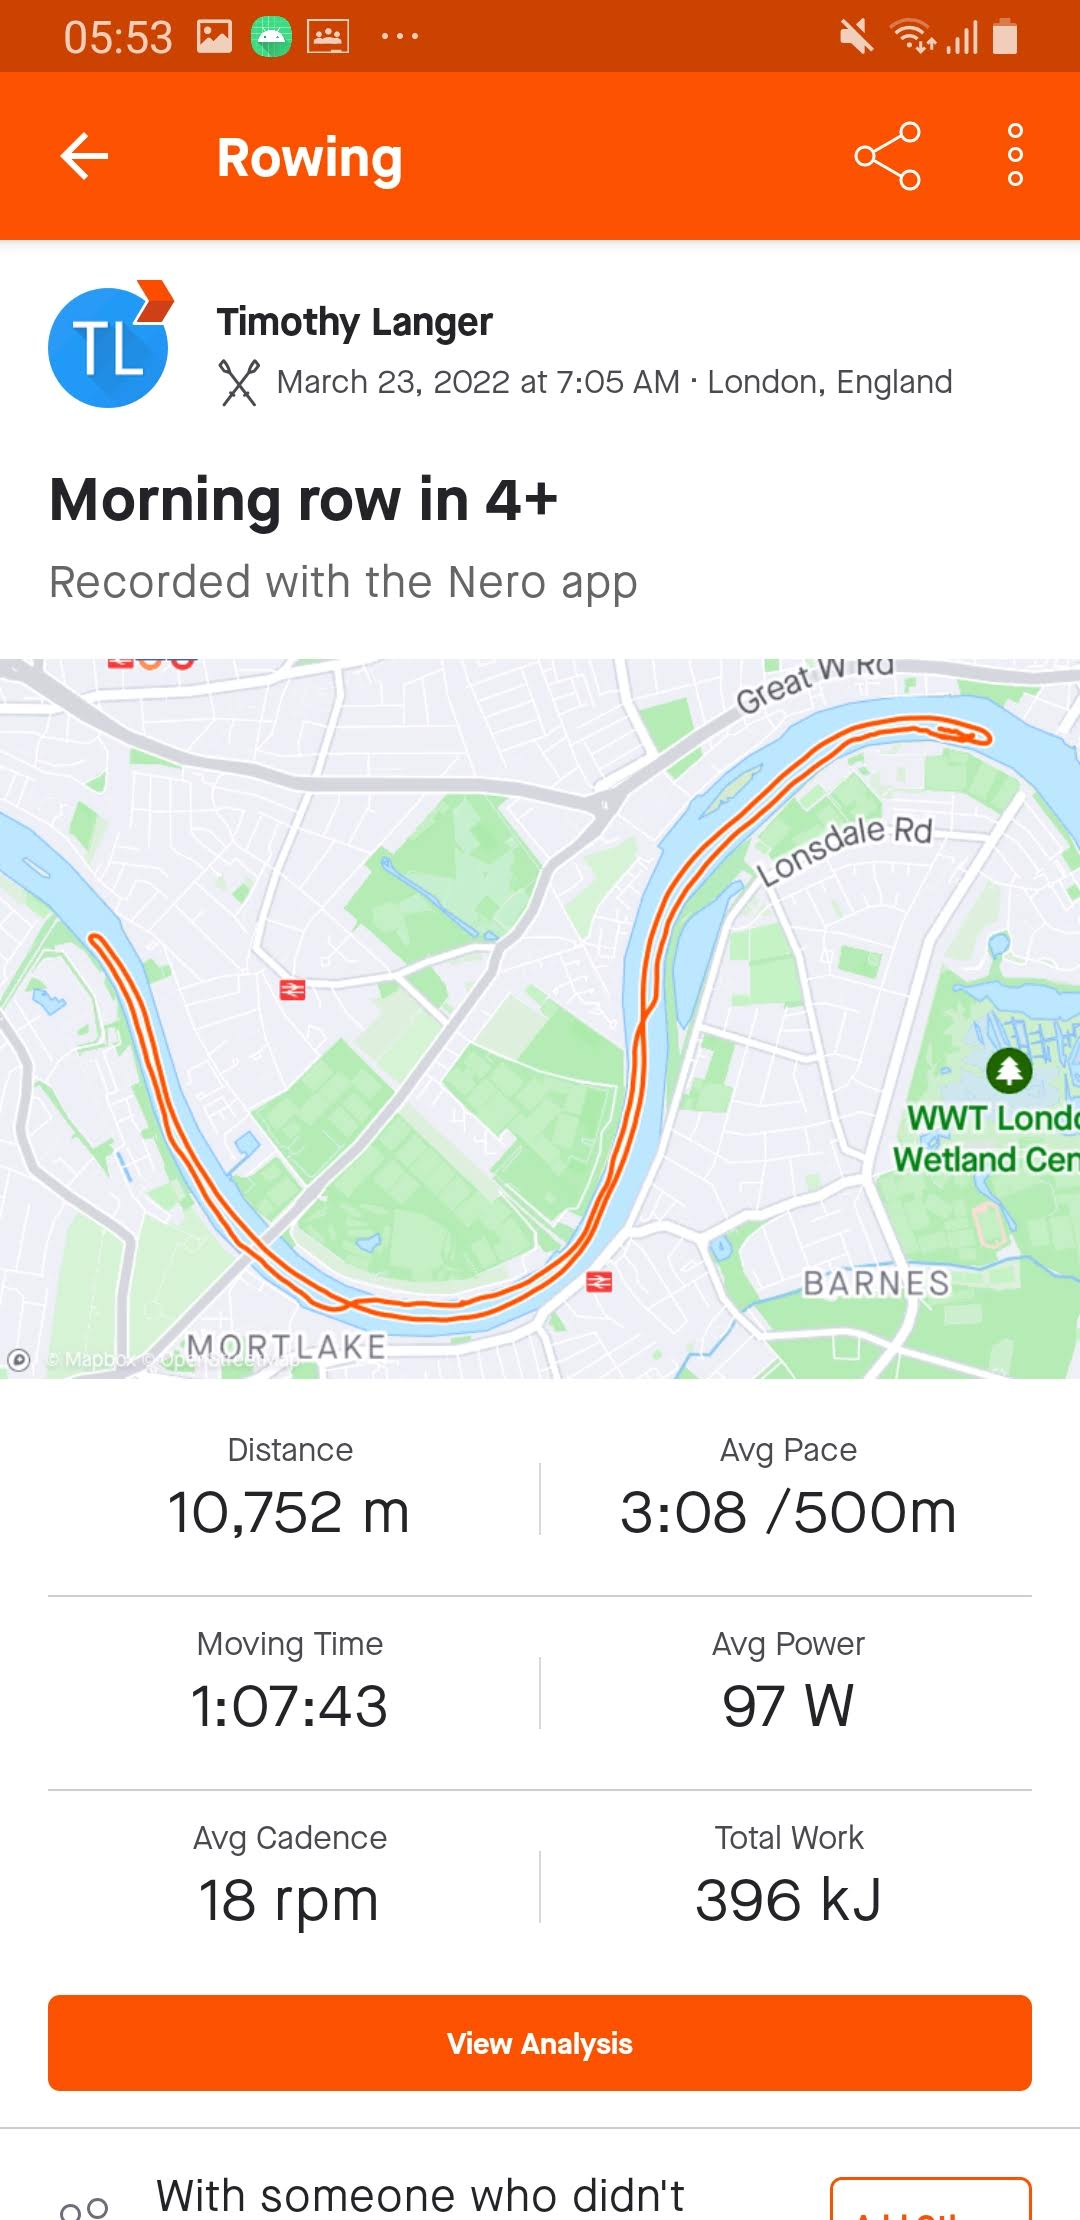
\includegraphics[width=0.3\textwidth]{strava.jpg}
  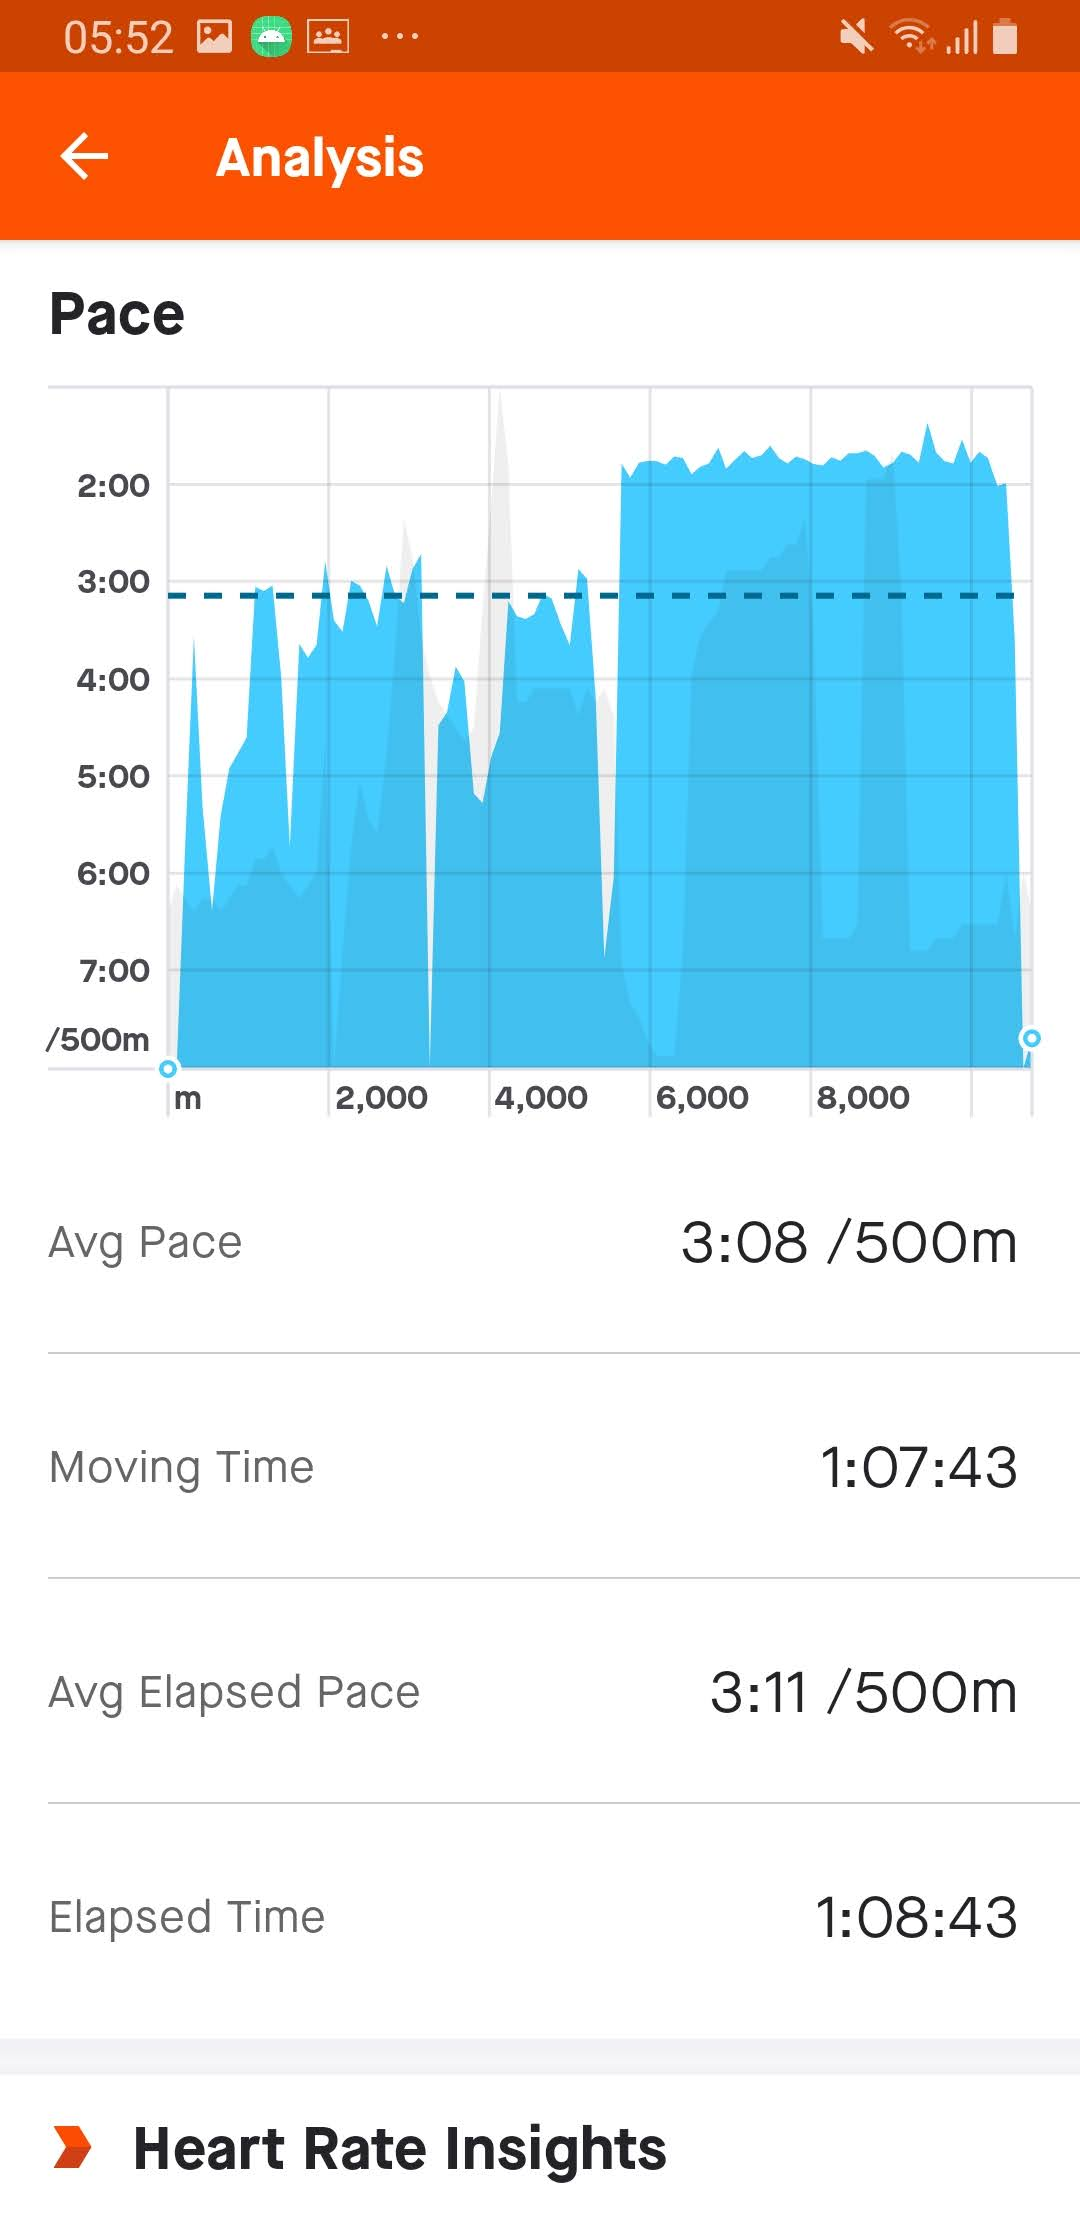
\includegraphics[width=0.3\textwidth]{stravapace.jpg}
  \caption{Strava session overview / pace analysis}
  \label{fig:stravathing}
\end{figure}

\begin{figure}[h!]
  \centering
  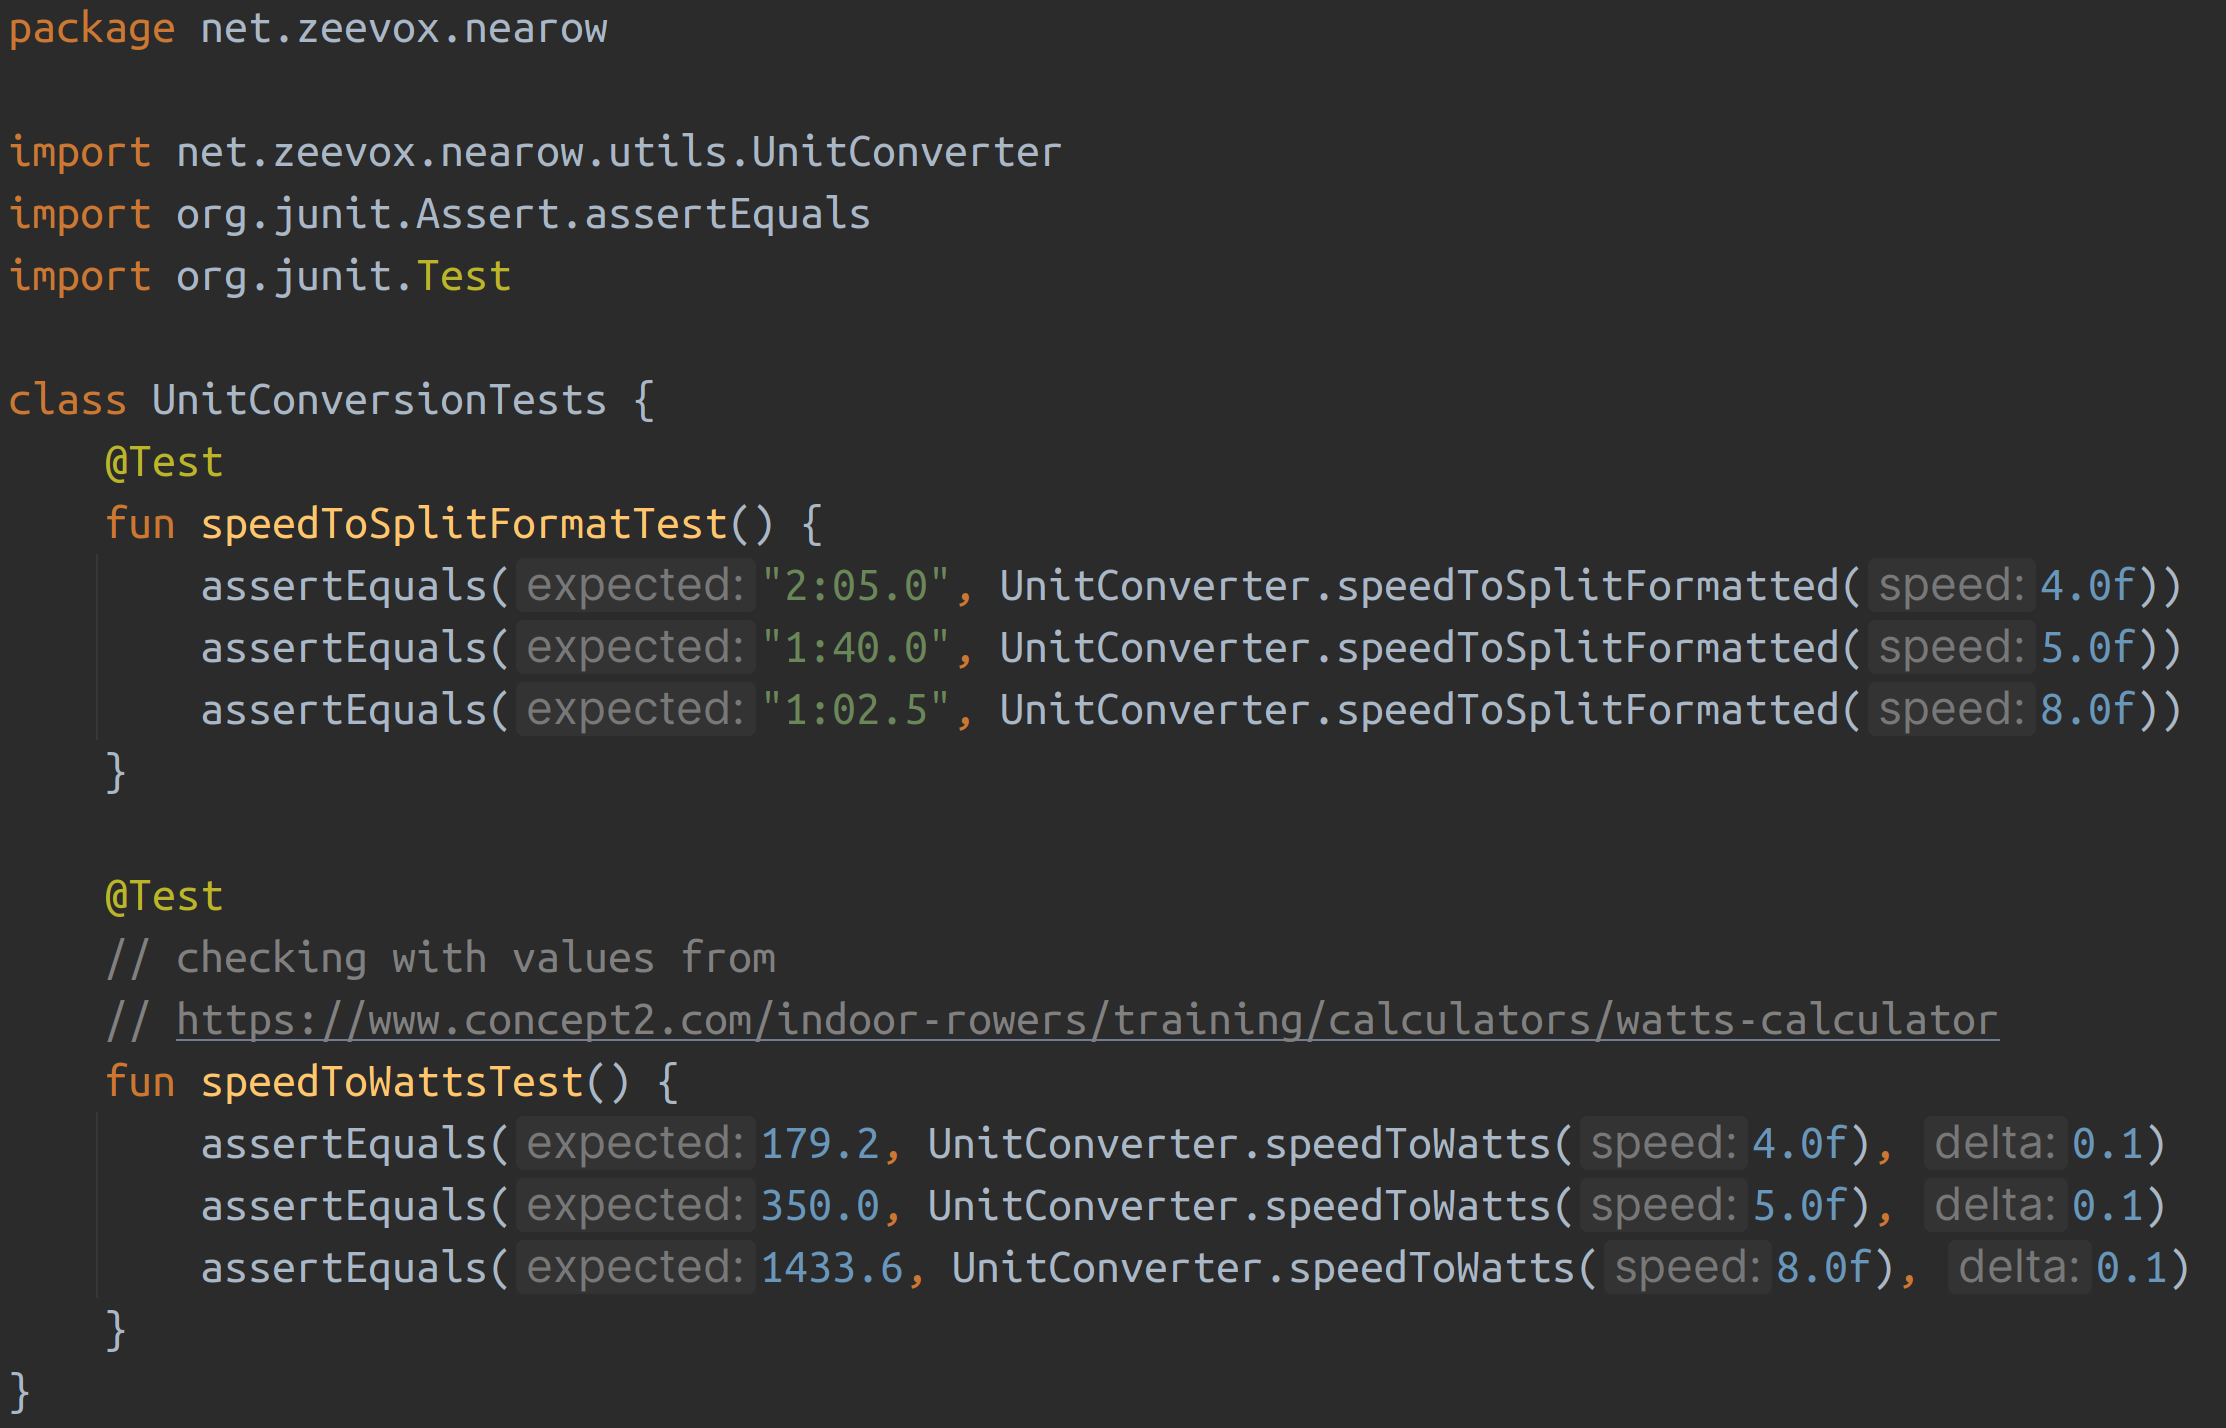
\includegraphics[width=0.7\textwidth]{code-UnitConversionTests.png}
  \caption{Unit tests for the \texttt{UnitConverter} class}
  \label{fig:UnitConversionTests}
\end{figure}

Unlike many of the other parts of this application, the \texttt{UnitConverter} class can actually be tested with unit tests in the \texttt{UnitConversionTests} class. The JUnit testing library was selected for its simplicity and good integration with the Android Studio development environment. Speed to split and speed to power conversion is tested, as shown in figure \ref{fig:UnitConversionTests}.

\chapter{Evaluation}

\section{Feedback from a 3rd party}

The application was installed on a OnePlus 8T belonging to James Trotman (interviewed earlier) and his opinion was requested after a training session in the eight. He trialled the application on his device alongside an NK SpeedCoach; the results were discussed after the outing. 

The user found their way around the app very quickly. The only note to make is that, as on installation there were no already recorded sessions, the purpose of the blank screen shown in the "view sessions" menu was not clear.

James said that the stroke rate was rather accurate, always within a single spm of the stroke rate given by the SpeedCoach. He did comment that the split, however, was rather jumpy, and was not as good as the SpeedCoach; according to James, it was oscillating around the same split as the SpeedCoach, but only accurate, as per his estimate, to the nearest $10$ seconds. It is proposed that this is because the SpeedCoach samples the split once per stroke, whereas the application samples once per second, which, at low stroke rates, results in several samples being taken per stroke. This means that it reports a slower split on the recovery and a fast split on the drive. This could be corrected by implementing a moving average or changing the GPS client to perform sampling as a function of the rate.

Battery usage was also discussed. James' phone battery decreased by around $40\%$ over the course of a two-hour row. Although not a major concern, we agreed that ideally battery usage should be decreased. The screen is the major factor for battery drain, and on a sunny day the high brightness further causes increased battery consumption. This could be targeted by, for example, giving the UI a black background to reduce battery usage on OLED screens.

\section{Objectives analysis}

The specification described in section \ref{sec:spec} is copied below, augmented with a discussion of the achievements of the application.

\begin{enumerate}
  \item be an application installable on any modern Android smartphone,
  
  \textit{The application was tested on several Android devices: a Pixel 2 (2017), a Pixel 4a 5G (2020), James' OnePlus 8T (2020) and a Samsung Galaxy S8 (2017). No device-specific issues were discovered.}
  \item require minimal configuration and interaction from the end user, and ideally none at all,
 
  \textit{The application is started up and starts measuring stroke rate and split immediately. The only initial configuration required is a request to access the user's GPS location. The application does not require any user interaction once recording is started.}
  \item be as easy to use and self-explanatory as possible for a new user,
  
  \textit{James found his way around the application very quickly. He mentioned that he liked the long-press requirement for the stop button.}
  \item calculate the following metrics, as accurately as possible:
  \begin{itemize}
    \item the boat's stroke rate,
    
    \textit{The application calculated stroke rate is accurate to within a single spm of the stroke rate given by the SpeedCoach. The SpeedCoach, however, does excel in picking up stroke rate changes almost instantaneously, whereas the application could take up to 10 seconds for particularly sudden changes in stroke rate.}
    \item the boat's split,
    
    \textit{The average boat split as found by the application is very close to that calculated by the SpeedCoach. However, realtime stroke rate is not as accurate as the SpeedCoach.}
    \item the total distance rowed over the course of the session,
    
    \textit{The SpeedCoach does not measure distance covered while drifting with the current. The application does, which means that the distance covered is higher. However, this does not make it inaccurate.}
  \end{itemize}
  \item display the above metrics in a realtime and an easy-to-read manner,
  
  \textit{Metrics are updates once per second, which is more than enough. Potentially even too often, which is why split can seem to jump around.}
  \item collect data during a rowing session using nothing but the hardware on the smartphone,
  
  \textit{The application does not require any additional hardware. A waterproof case may be a requirement for some, but it is not necessary for the functionality.}
  \item provide start/stop functionality to record the rowing session for later review,
  
  \textit{A start/stop button is provided. Sessions are recorded to a database.}
  \item allow the user to export the recorded rowing session as a \href{https://developer.garmin.com/fit/file-types/activity/}{\texttt{FIT} activity file} that can be imported into 3rd-party software, such as \href{https://strava.com}{Strava}, containing
  \begin{itemize}
    \item the geolocation of the boat,
    \item the speed of the boat,
    \item the cadence, or stroke rate, of the rowers,
    \item the estimated power generated by the rowers
  \end{itemize}

  \textit{FIT activity export functionality is present. Files generated by the application can be imported into Strava and viewed on a map alongside a chart of split.}
  \item be as battery-efficient as possible
  
  \textit{Optimisations have been made and algorithms carefully considered to make them as battery-efficient as possible. Perhaps the UI could be adapted to reduce the battery drain caused by a bright white screen.}
\end{enumerate}

\chapter{Appendix}

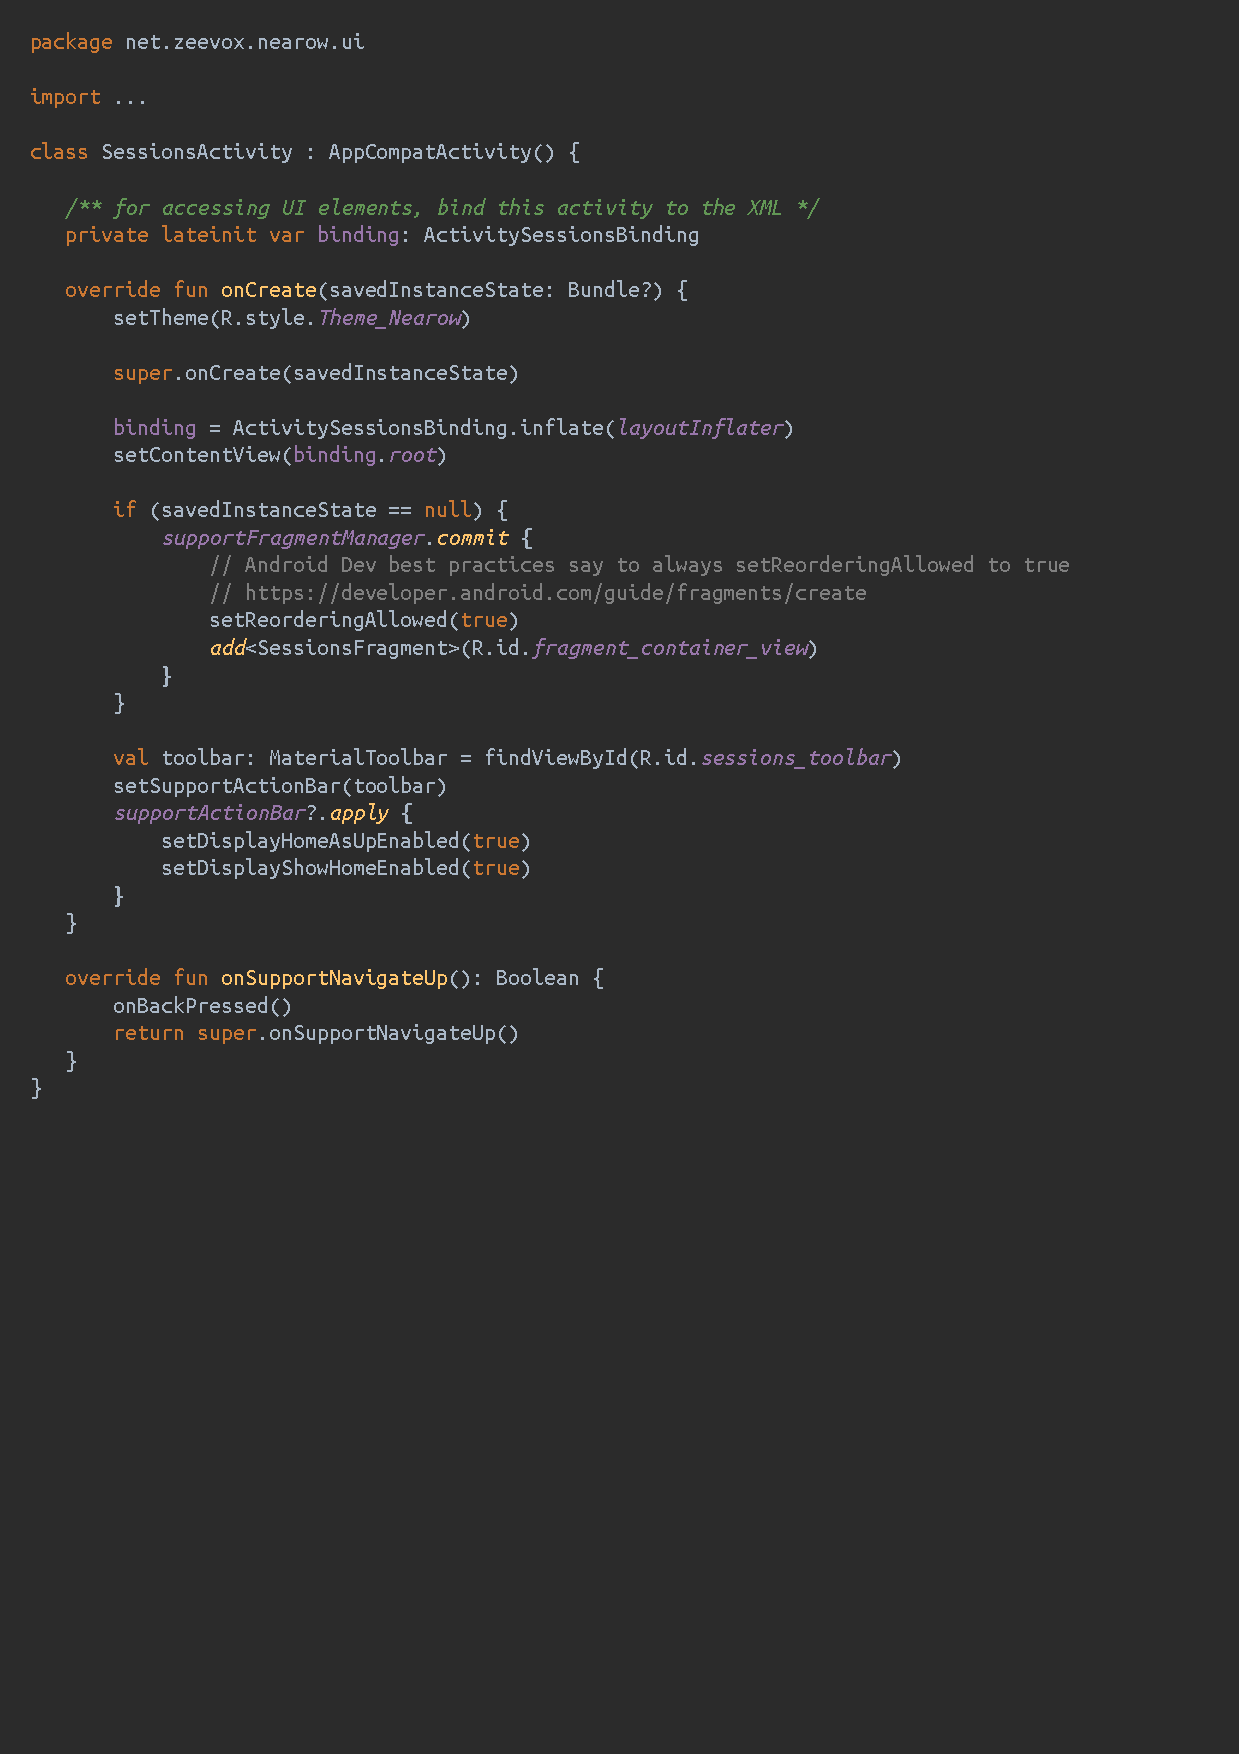
\includepdf[pages=-,pagecommand={\invisiblesection{\texttt{SessionsActivity.kt}} \label{SessionsActivity}},width=1.0\textwidth]{code/SessionsActivity.pdf}
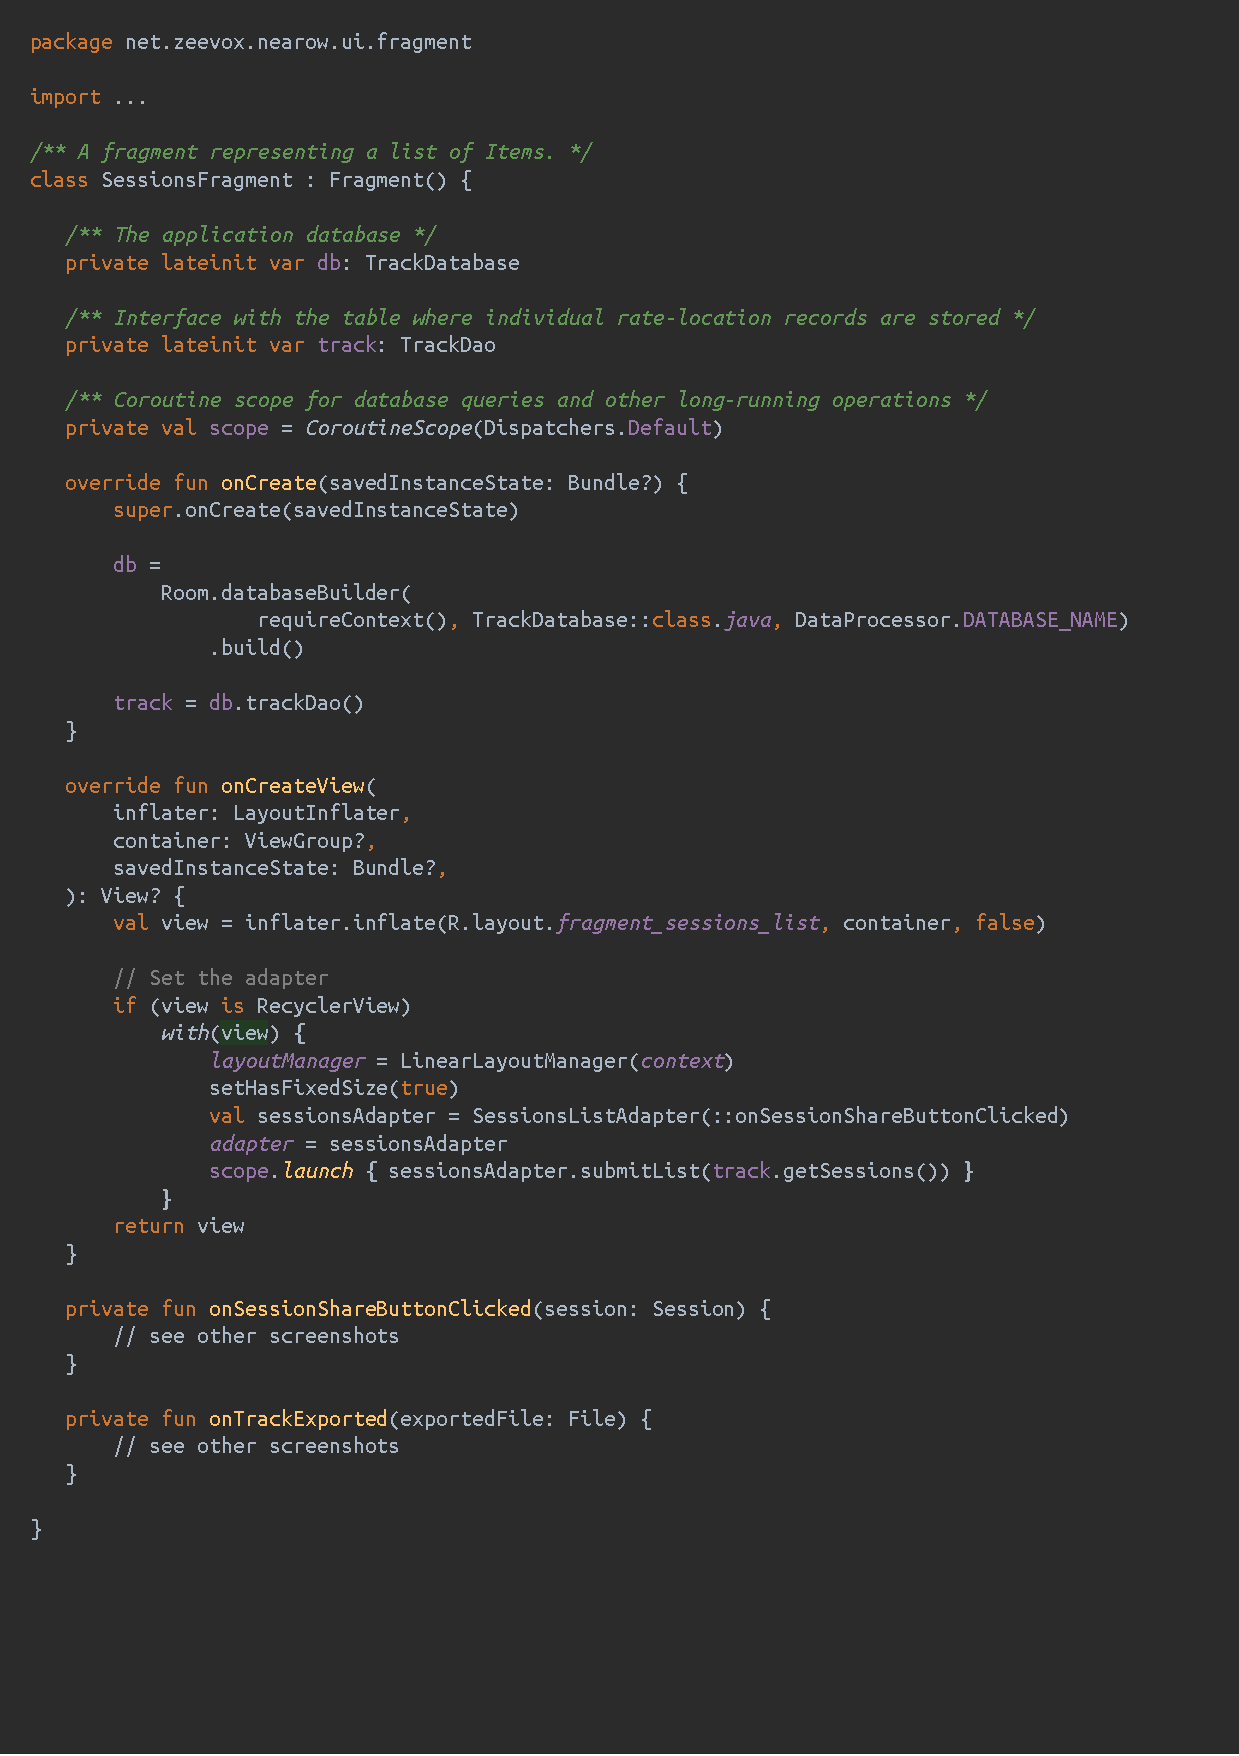
\includepdf[pages=-,pagecommand={\invisiblesection{\texttt{SessionsFragment.kt}} \label{SessionsFragment}},width=1.0\textwidth]{code/SessionsFragment.pdf}
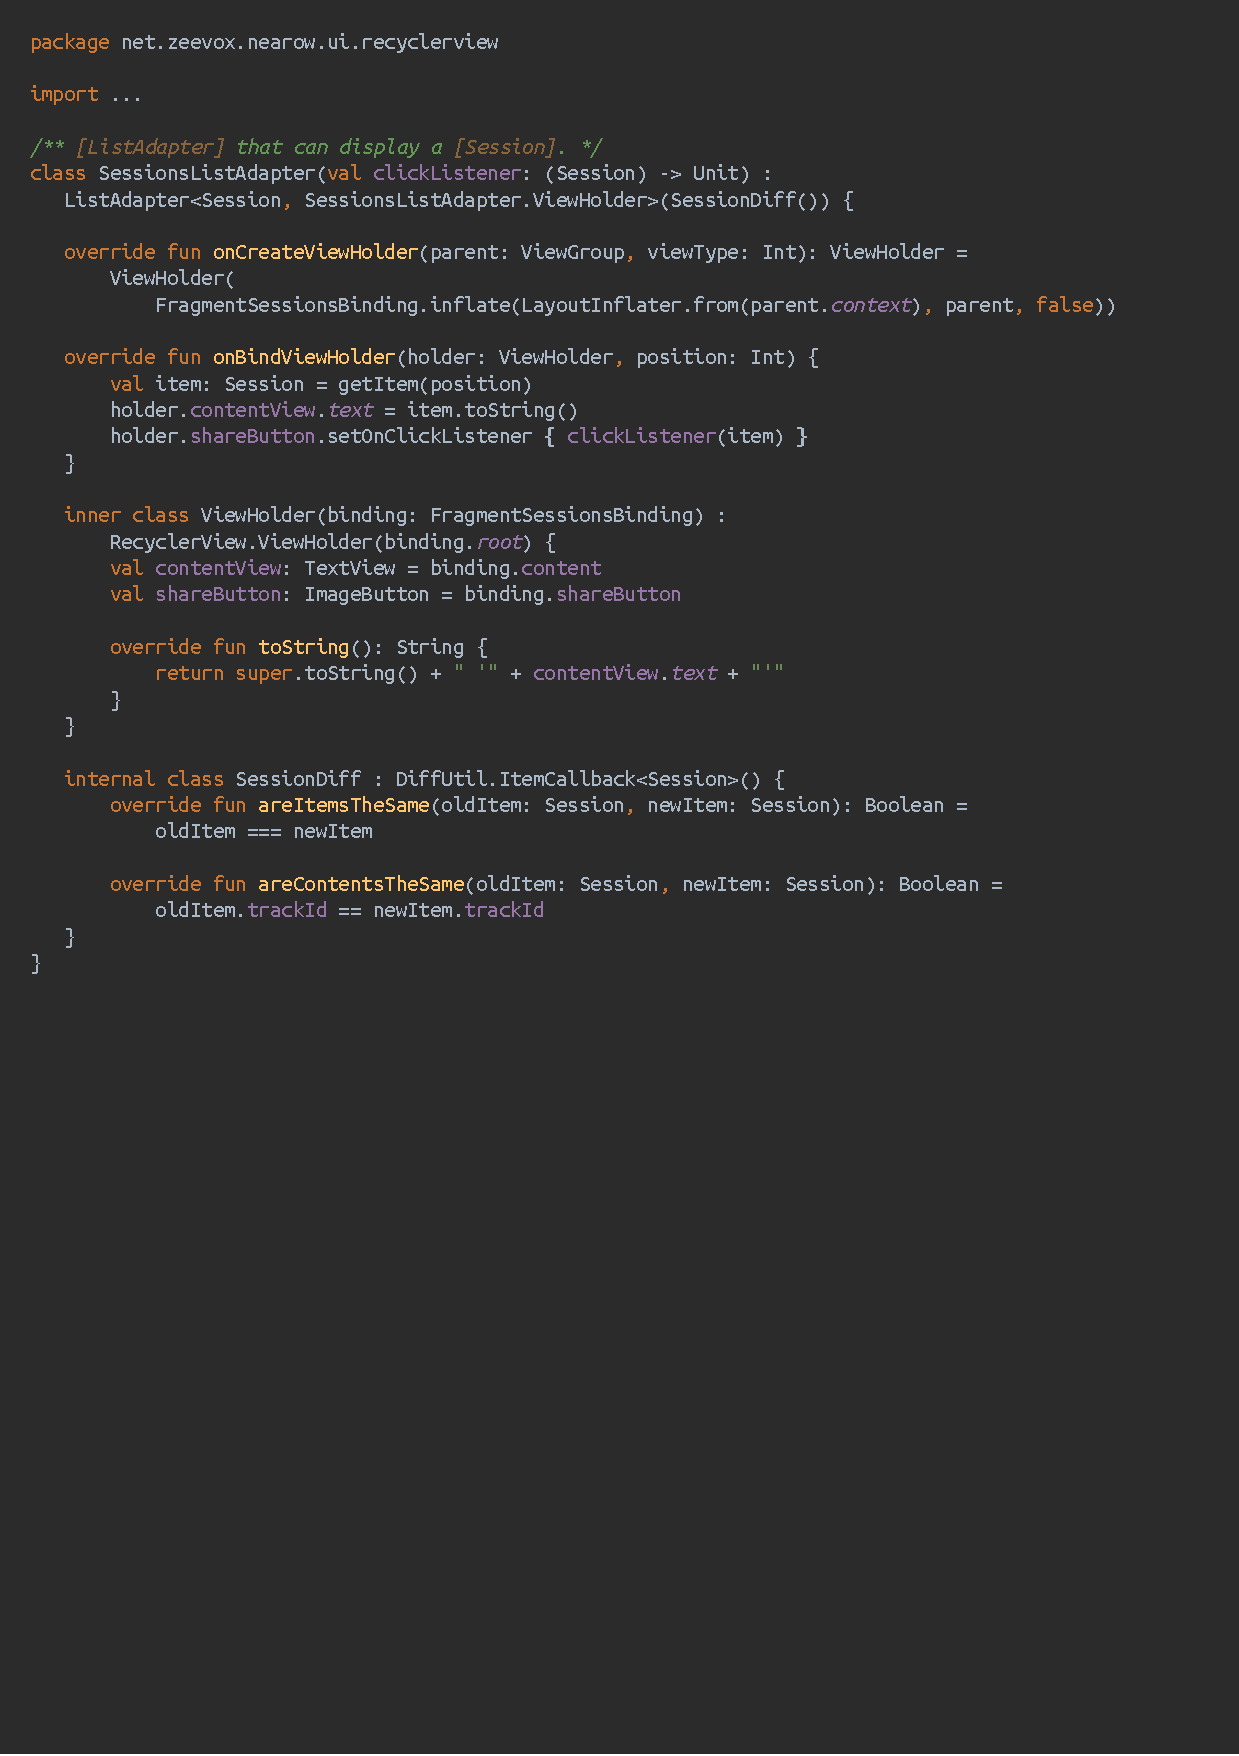
\includepdf[pages=-,pagecommand={\invisiblesection{\texttt{SessionsListAdapter.kt}} \label{SessionsListAdapter}},width=1.0\textwidth]{code/SessionsListAdapter.pdf}

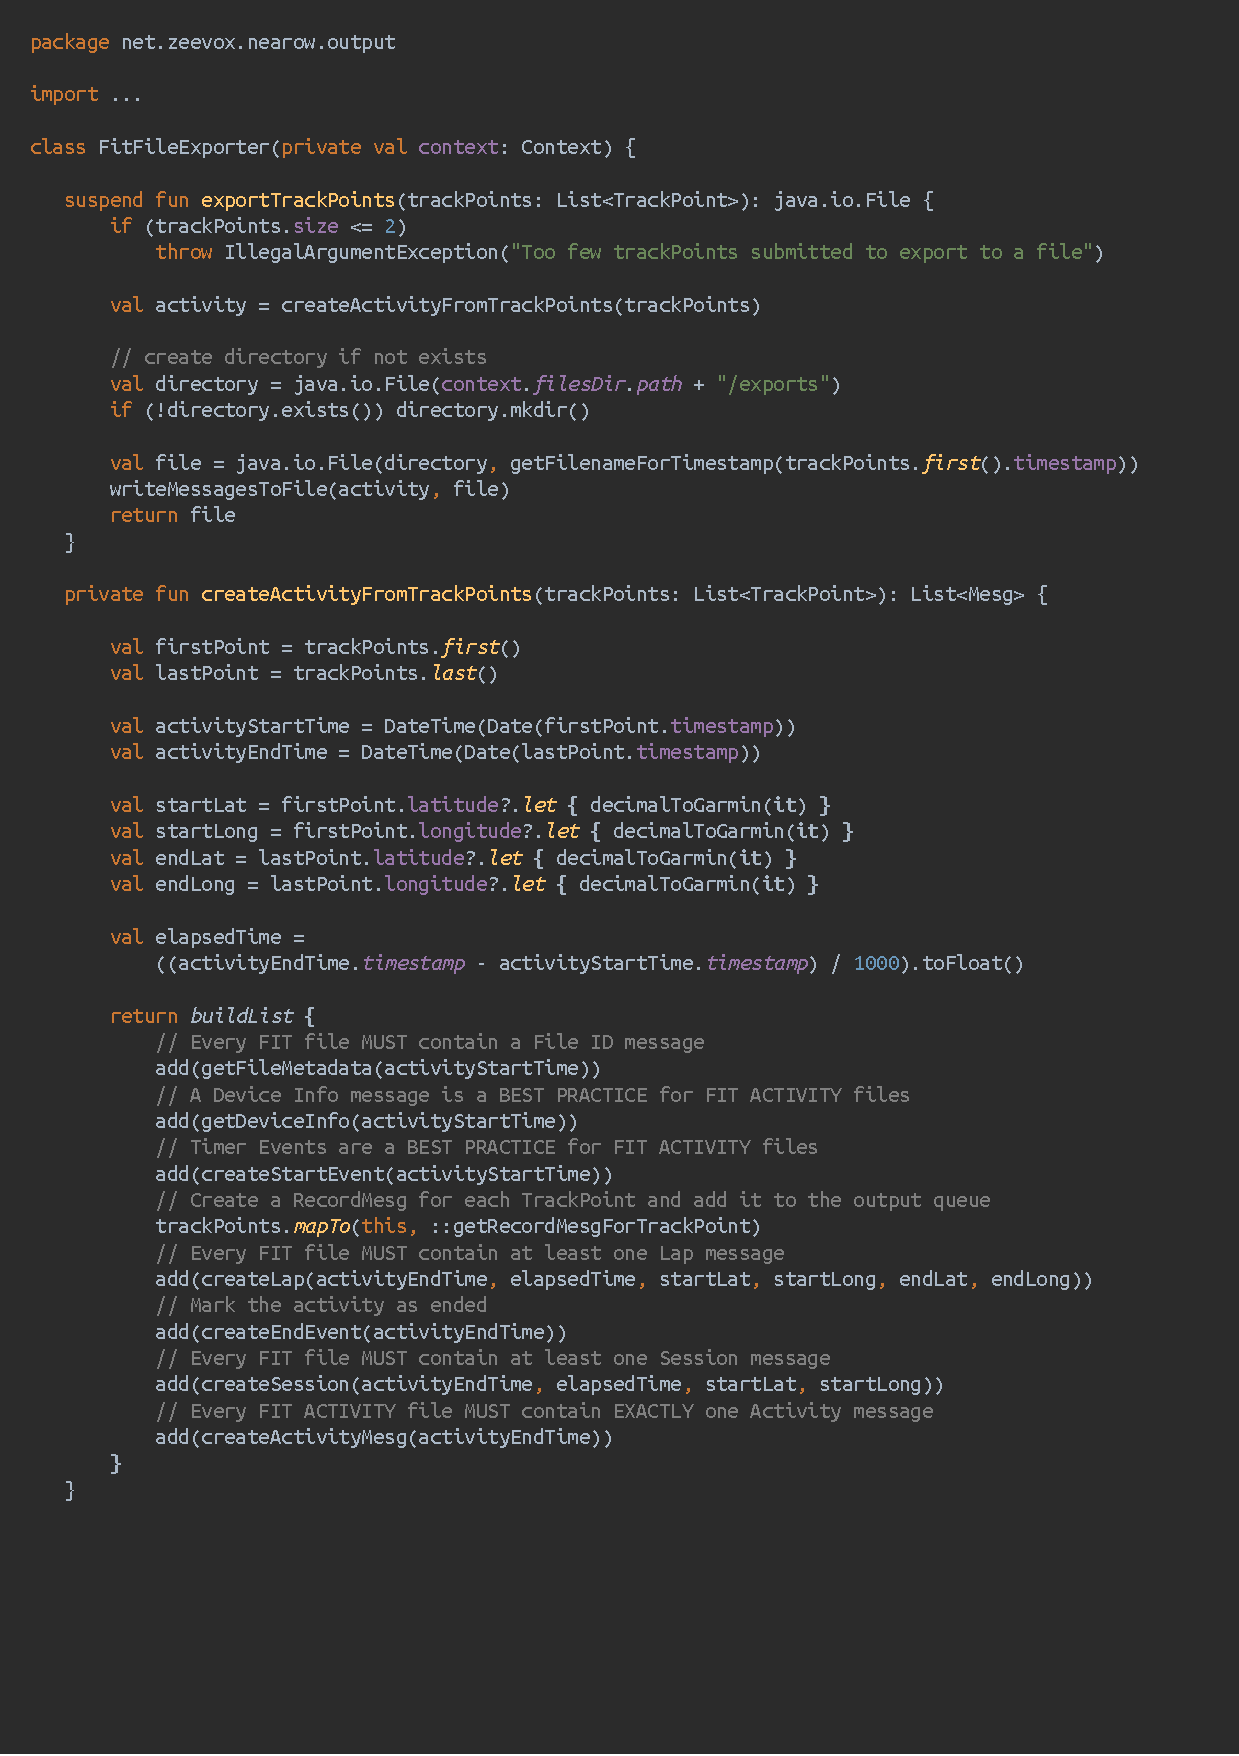
\includepdf[pages=1,pagecommand={\invisiblesection{\texttt{FitFileExporter.kt}} \label{FitFileExporterStart}},width=1.0\textwidth]{code/FitFileExporter.pdf}
\includepdf[pages=2-,pagecommand={},width=1.0\textwidth]{code/FitFileExporter.pdf}

\nocite{holten_imagick-ft_2020}
\nocite{noauthor_android_nodate}
\nocite{noauthor_android_nodate-1}
\nocite{noauthor_services_nodate}
\nocite{noauthor_sharing_nodate}
\nocite{noauthor_create_nodate}
\nocite{noauthor_request_nodate}
\nocite{noauthor_java_nodate}

\printbibliography[heading=bibintoc]

\end{document}
